%==================================================================================================
\chapter{Formulação numérica para mecânica dos Fluidos} \label{EGDF}
%==================================================================================================

No presente capítulo serão apresentadas as equações que governam os escoamentos isotérmicos incompressíveis. Inicialmente apresenta-se a formulação escrita em uma descrição Euleriana, onde se considera um domínio fixo com referência à condição atual do escoamento (Seção \ref{CFD-E}). Em seguida essa formulação será expandida para uma descrição Lagrangiana-Euleriana Arbitrária (ALE), onde será possível realizar a movimentação independente do domínio do fluido (Seção \ref{CFD-ALE}). Posteriormente essas equações acarretarão, a partir do método dos resíduos ponderados, na formulação semi-discreta do problema (Seção \ref{FSD}), sendo a forma estabilizada pelo método \VMS (VMS) apresentada na seção \ref{VMS}.

%==================================================================================================
\section{Descrição Euleriana} \label{CFD-E}
%==================================================================================================

Em uma descrição Euleriana é possível se obter uma expressão que defina a conservação de massa (também denominada como Equação da Continuidade) do fluido, considerando um elemento infinitesimal permeável, que definirá o volume de controle, conforme ilustrado na Figura \ref{fig:BalMas}, em que $\BB{u}$ é o valor da velocidade na posição atual $\BB{y}$ e $\rho$ é a massa específica do fluido nesse ponto.

\begin{figure}[h!]
    \centering
    \caption{Taxa de fluxo de massa em um elemento infinitesimal permeável.}
    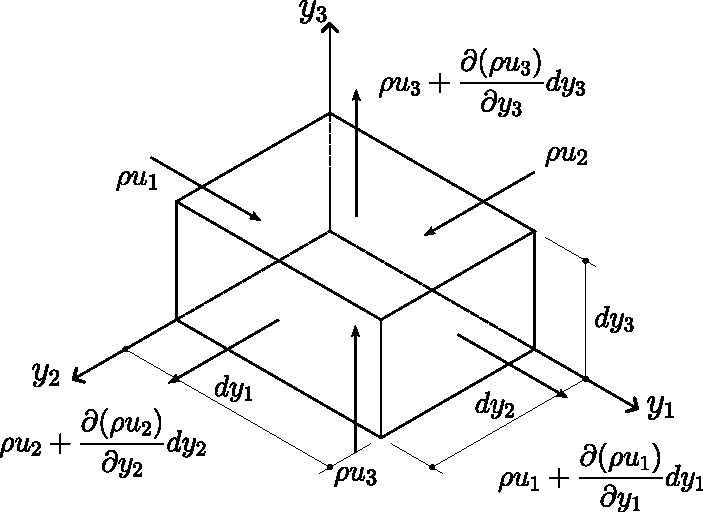
\includegraphics[width=.5\linewidth]{Figuras/BalMas.pdf}
    \\Fonte: Autoria Própria (\the\year).
    \label{fig:BalMas}
\end{figure}

Realizando-se o balanço de massa nesse elemento tem-se:

\begin{equation}
    dm=dm_0+\apdery{dm}{t}dt\text{,}
\end{equation}

\noindent que resulta em uma expressão simplificada dada por \eqref{eq:BalMas}, que representa a conservação de massa em um elemento infinitesimal.

\begin{equation}
    \frac{D\rho}{Dt}+\rho \Ny\cdot\BB{u}=\dvt{\rho}+\Ny\cdot(\rho \BB{u})=0\text{,}
    \label{eq:BalMas}
\end{equation}

\noindent sendo $D\rho/Dt$ a derivada material, definida para um escalar $\phi$ qualquer como:

\begin{equation}
    \frac{D\phi}{Dt}=\dvt{\phi}+\BB{u}\cdot\Ny\phi\text{,}
\end{equation}

\noindent em que $\Ny\cdot(\cdot)$ é o operador divergente e $\Ny(\cdot)$ é o operador gradiente, que para uma função escalar $g$ é definido por \eqref{eq:grad1} e para uma função vetorial é definido por \eqref{eq:grad2}:

\begin{subequations}
    \begin{align}
         & \Ny g=\der{g}{\BB{y}}\equiv\der{g}{y_i}            &  & \text{, com }i=1,2,\hdots,n_{sd}\text{ e} \label{eq:grad1}    \\
         & \Ny\BB{g}=\der{\BB{g}}{\BB{y}}\equiv\der{g_i}{y_j} &  & \text{, com }i\text{ e }j=1,2,\hdots,n_{sd}, \label{eq:grad2}
    \end{align}
\end{subequations}

\noindent sendo $n_{sd}=2$ ou $3$ a dimensão do problema em análise.

Para escoamentos incompressíveis a equação da continuidade pode ser reduzida a:

\begin{equation}
    \Ny\cdot\BB{u}=0\text{,}\label{eq:incomp}
\end{equation}

\noindent denominada como condição de incompressibilidade.

Já a equação que expressa a Conservação da Quantidade de Movimento linear (ou de \textit{Momentum} Linear) pode ser obtida ao se considerar a taxa de fluxo de quantidade de movimento no elemento infinitesimal permeável, ilustrado na Figura \ref{fig:ConQtdMov}.

\begin{figure}[h!]
    \centering
    \caption{Taxa de fluxo de quantidade de movimento em um elemento infinitesimal permeável.}
    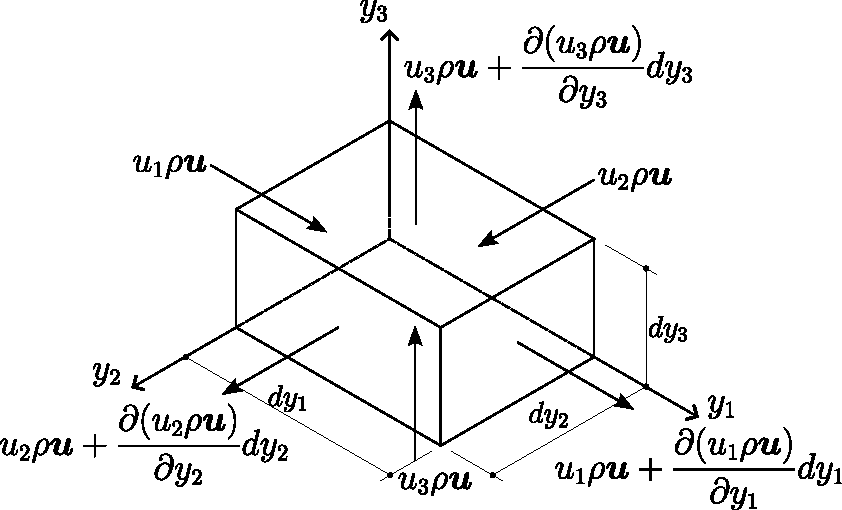
\includegraphics[width=.55\linewidth]{Figuras/ConQtdMov.pdf}
    \\Fonte: Autoria Própria (\the\year).
    \label{fig:ConQtdMov}
\end{figure}

Assim, procede-se com o balanço da taxa de quantidade de movimento, tendo-se uma resultante de forças externas atuante no elemento dado por $d\BB{F}$. Logo, após feitas as devidas simplificações, chega-se à equação:

\begin{equation}
    \apdery{(\rho \BB{u})}{t}+\Ny\cdot(\rho \BB{u}\otimes\BB{u})-\BB{q}=\BB{0}\text{,}
    \label{eq:ConQtdMov}
\end{equation}

\noindent em que $\BB{q}$ representa a força resultante por unidade de volume, ou seja, $\BB{q}=d\BB{F}/dV$. Entretanto, não é de interesse escrever a equação \eqref{eq:ConQtdMov} em termos desse vetor $\BB{q}$, mas em termos do tensor de tensões de Cauchy ($\tens$) e forças de volume. Para isso, considera-se o diagrama de corpo livre do elemento infinitesimal ilustrado na Figura \ref{fig:EqFor}, onde são representadas apenas as componentes de tensão e de forças de volume atuantes na direção $y_1$.

\begin{figure}[h!]
    \centering
    \caption{Componentes de forças atuantes no elemento infinitesimal na direção $y_1$.}
    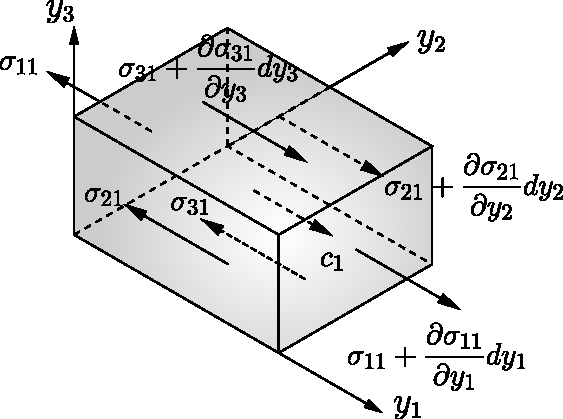
\includegraphics[width=.5\linewidth]{Figuras/EqFor.pdf}
    \\Fonte:Autoria Própria (\the\year).
    \label{fig:EqFor}
\end{figure}

Fazendo o equilíbrio de forças nessa direção, obtém-se que:

\begin{equation}
    q_1=\der{\sigma_{11}}{y_1}+\der{\sigma_{21}}{y_2}+\der{\sigma_{31}}{y_3}+c_1\text{,}
\end{equation}

\noindent a qual pode ser estendida analogamente para as demais direções, e sabendo-se da simetria de $\tens$, tem-se:

\begin{equation}
    \BB{q}=\Ny\cdot\tens+\BB{c}\text{.}
    \label{eq:RelQSig}
\end{equation}

Substituindo \eqref{eq:RelQSig} em \eqref{eq:ConQtdMov} e aplicando a condição de incompressibilidade obtém-se a equação da conservação da quantidade de movimento escrita em termos de tensões:

\begin{equation}
    \rho\bigpar{\dvt{\BB{u}}+\BB{u}\cdot\Ny\BB{u}-\BB{f}}-\Ny\cdot\tens=\BB{0}\text{,}
    \label{eq:ConQtdMov-2}
\end{equation}

\noindent em que $\BB{c}=\rho\BB{f}$, tal que $\BB{f}$ é uma força por unidade de massa. Além disso, também é possível escrever a equação \eqref{eq:ConQtdMov-2} utilizando a notação de derivada material como:

\begin{equation}
    \rho\bigpar{\frac{D\BB{u}}{Dt}-\BB{f}}-\Ny\cdot\tens=\BB{0}\text{.}
    \label{eq:ConQtdMov-3}
\end{equation}

Já o domínio em que essas equações são válidas pode ser definido como $\Omega\subset\mathbb{R}^{n_{sd}}$, tal que $\Omega$ possui uma fronteira $\Gamma=\partial\Omega$, em que a parte dessa fronteira onde se impõem condições cinemáticas é denominada como fronteira de Dirichlet ($\Gamma_D$) e a parte onde há prescrição de forças de superfície é denotado como fronteira de Neumann ($\Gamma_N$), conforme pode ser visualizado na Figura \ref{fig:Dom}.

\begin{figure}[h!]
    \centering
    \caption{Domínio de análise e fronteiras consideradas para problemas de mecânica dos fluidos.}
    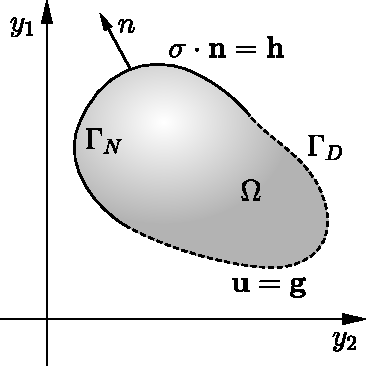
\includegraphics[width=.35\linewidth]{Figuras/Dom}
    \\Fonte: Autoria Própria (\the\year).
    \label{fig:Dom}
\end{figure}

Dessa forma, o problema a ser resolvido pode ser escrito a partir das equações:

\begin{equation}
    \left\{
    \begin{array}{ll}
        \rho\bigpar{\dvt{\BB{u}}+\BB{u}\cdot\Ny\BB{u}-\BB{f}}-\Ny\cdot\tens=\BB{0} & \text{ em }\Omega\text{,}   \\
        \Ny\cdot\BB{u}=0                                                           & \text{ em }\Omega\text{,}   \\
        \tens\cdot\BB{n}=\BB{h}                                                    & \text{ em }\Gamma_N\text{,} \\
        \BB{u}=\BB{g}                                                              & \text{ em }\Gamma_D\text{,}
    \end{array}
    \right.\label{eq:NS-Euler}
\end{equation}

\noindent as quais são chamadas de equações de Navier-Stokes para escoamentos incompressíveis em descrição Euleriana \cite{bazilevs2013computational,bazilevs2010large,bazilevs2007variational,hughes2002variational,hughes2000large}.

%==================================================================================================
\section{Descrição Lagrangiana-Euleriana Arbitrária} \label{CFD-ALE}
%==================================================================================================

A descrição Lagrangiana-Euleriana Arbitrária (\textit{Arbitrary Lagrangian-Eulerian} - ALE) originou-se do trabalho de \citeonline{donea1982arbitrary}. São considerados 3 domínios, $\Omega_0$, $\Omega$ e $\hat{\Omega}$, que representam os domínios do contínuo em sua configuração inicial e atual e o domínio da malha respectivamente, como ilustrado na Figura \ref{Fig:ALE}. O domínio $\hat{\Omega}$ possui movimento arbitrário.

\begin{figure}[h!]
    \centering
    \caption{Descrição Lagrangiana-Euleriana Arbitrária.}
    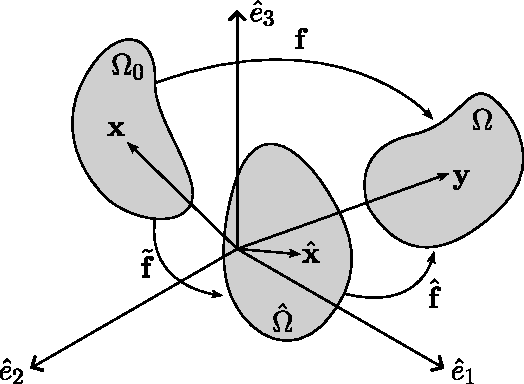
\includegraphics[width=.45\linewidth]{Figuras/ALE.pdf}
    \label{Fig:ALE}
    \\Fonte: Autoria Própria (\the\year).
\end{figure}

%\parei aquiiiii

As coordenadas $\BB{x}$, $\BB{y}$ e $\HBB{x}$ representam as coordenadas de um ponto nos domínios $\Omega_0$, $\Omega$ e $\hat{\Omega}$, respectivamente. Já as funções $\BB{f}(\BB{x},t)=\BB{y}(\BB{x},t)$, $\TBB{f}(\BB{x},t)=\HBB{x}(\BB{x},t)$ e $\HBB{f}(\HBB{x},t)=\BB{y}(\HBB{x},t)$ são funções de mudança de configuração.

Com isso, pode-se obter o gradiente das funções de mudança de configuração:

\begin{subequations}
    \begin{equation}
        \mathbf{A}=\der{(\BB{f}(\BB{x},t),t)}{(\mathbf{x},t)}=\begin{bmatrix}
            \der{\BB{y}}{\BB{x}} & \BB{u} \\\BB{0}^T&1
        \end{bmatrix}\text{,}\label{F2}
    \end{equation}
    \begin{equation}
        \TBB{A}=\der{(\TBB{f}(\BB{x},t),t)}{(\BB{x},t)}=\begin{bmatrix}
            \der{\HBB{x}}{\BB{x}} & \BB{w} \\\BB{0}^T&1
        \end{bmatrix}\text{, e}\label{F1}
    \end{equation}
    \begin{equation}
        \HBB{A}=\der{(\HBB{f}(\HBB{x},t),t)}{(\HBB{x},t)}=\begin{bmatrix}
            \der{\BB{y}}{\HBB{x}} & \uhat \\\BB{0}^T&1
        \end{bmatrix}\text{,}\label{F3}
    \end{equation}
    \label{eq:GradFun}
\end{subequations}

\noindent nos quais $\BB{u}=\partial\BB{y}/\partial t|_{\BB{x}}$, $\BB{w}=\partial\HBB{x}/\partial t|_{\BB{x}}$ e $\uhat=\partial\HBB{f}/\partial t|_{\HBB{x}}$. Além disso, vale ressaltar que $\BB{f}=\HBB{f}(\TBB{f},t)$, portanto $\BB{A}=\HBB{A}\cdot\TBB{A}$, ou seja:

\begin{equation}
    \begin{bmatrix}\der{\BB{y}}{\BB{x}}&\BB{u}\\\BB{0}^T&1\end{bmatrix}=
    \begin{bmatrix}\der{\BB{y}}{\HBB{x}}&\uhat\\\BB{0}^T&1\end{bmatrix}\cdot
    \begin{bmatrix}\der{\HBB{x}}{\BB{x}}&\BB{w}\\\BB{0}^T&1\end{bmatrix}\text{,}
    \label{F4}
\end{equation}

\noindent que possui, como uma de suas consequências:

\begin{equation}
    \BB{u}=\der{\BB{y}}{\HBB{x}}\cdot\BB{w}+\uhat\text{, ou}
    \label{u1}
\end{equation}

\begin{equation}
    \BB{w}=\der{\HBB{x}}{\BB{y}}\cdot(\BB{u}-\uhat)\text{.}
    \label{w1}
\end{equation}

Assim é possível definir a derivada material em uma descrição ALE. Para isso considere uma propriedade $\phi(\BB{y},t)$ escrita em termos da configuração atual, $\phi^*(\HBB{x},t)$ escrita em termos da configuração de referência e $\phi^{**}(\BB{x},t)=\phi^*(\TBB{f}(\BB{x},t),t)$ escrita em termos da configuração inicial. Logo:

\begin{equation}
    \der{\phi^{**}(\BB{x},t)}{(\BB{x},t)}=\der{\phi^*(\HBB{x},t)}{(\HBB{x},t)}\cdot\der{\TBB{f}(\BB{x},t)}{(\BB{x},t)}\text{, ou}
    \label{phi1}
\end{equation}

\begin{equation}
    \begin{bmatrix}\der{\phi^{**}}{\BB{x}}&\der{\phi^{**}}{t}\end{bmatrix}=
    \begin{bmatrix}\der{\phi^{*}}{\HBB{x}}&\der{\phi^{*}}{t}\end{bmatrix}\cdot
    \begin{bmatrix}\der{\HBB{x}}{\BB{x}}&\BB{w}\\\BB{0}^T&1\end{bmatrix}
    \text{.}
    \label{phi2}
\end{equation}

\noindent Portanto:

\begin{equation}
    \der{\phi^{**}}{t}=\der{\phi^{*}}{\HBB{x}}\cdot\BB{w}+\der{\phi^{*}}{t}\text{.}
    \label{phi3}
\end{equation}

Substituindo \ref{w1} em \ref{phi3}, obtém-se que:

\[\der{\phi^{**}}{t}=\der{\phi^{*}}{\HBB{x}}\cdot\der{\HBB{x}}{\BB{y}}\cdot(\BB{u}-\uhat)+\der{\phi^{*}}{t}\]

\[\der{\phi^{**}}{t}=\der{\phi^{*}}{t}+(\BB{u}-\uhat)\cdot\der{\phi^{*}}{\BB{y}}\]

Dessa maneira, remove-se os sobrescritos * e ** e define-se a derivada material na descrição ALE como:

\begin{equation}
    \frac{D\phi}{Dt}=\apderxh{\phi}{t}+(\BB{u}-\uhat)\cdot\Ny\phi\text{.}
    \label{eq:DerMat2}
\end{equation}

Com isso, substitui-se $\phi$ por $\rho$ e aplica-se a Equação \eqref{eq:DerMat2} em \eqref{eq:BalMas} para se obter a Equação da Continuidade na descrição ALE:

\begin{equation}
    \apderxh{\rho}{t}+(\BB{u}-\uhat)\cdot\Ny\rho+\rho\Ny\cdot\BB{u}=0\text{,}
    \label{ConMas4}
\end{equation}

Já a Equação da Conservação da Quantidade de Movimento na descrição ALE pode ser obtida substituindo-se a Equação \eqref{eq:DerMat2} em \eqref{eq:ConQtdMov-3}, em que $\mathbf{\phi}=\mathbf{u}$, obtendo-se:

\begin{equation}
    \rho\left(\apderxh{\BB{u}}{t}+(\BB{u}-\uhat)\cdot\Ny\BB{u}-\BB{f}\right)-\Ny\cdot\tens^T=\BB{0}\text{.}
    \label{ConQtdMov10}
\end{equation}

Assim, pode-se escrever o problema a ser resolvido a partir das equações:

\begin{equation}
    \left\{
    \begin{array}{ll}
        \rho\bigpar{\dot{u}_i+(u_j-\hat{u}_j)u_{i,j}-f_i}-\sigma_{ji,j}=0 & \text{ em }\Omega\text{,}   \\
        u_{i,i}=0                                                         & \text{ em }\Omega\text{,}   \\
        \sigma_{ij}n_i=h_j                                                & \text{ em }\Gamma_N\text{,} \\
        u_j=g_j                                                           & \text{ em }\Gamma_D\text{,}
    \end{array}
    \right.\label{eq:NS-ALE}
\end{equation}

\noindent que são denominadas como as equações de Navier-Stokes para escoamentos incompressíveis em descrição ALE \cite{bazilevs2013computational}.

%==================================================================================================
\section{Modelo Constitutivo} \label{MC}
%==================================================================================================

O modelo constitutivo que relaciona o tensor de tensões de Cauchy com os campos de velocidade e de pressão é expresso de acordo com a Equação \eqref{eq:const1}:

\begin{equation}
    \sigma_{ij}=\tau_{ij}-p\delta_{ij}\text{,}\label{eq:const1}
\end{equation}

\noindent no qual $\tau_{ij}$ é o tensor de tensões viscosas (ou tensor desviador), que para fluidos Newtonianos é dado por:

\begin{equation}
    \tau_{ij}=\script{D}_{ij\alpha\beta}\dot{\varepsilon}_{ij}\text{,}
\end{equation}

\noindent em que $\script{D}_{ij\alpha\beta}$ é o tensor constitutivo de quarta ordem:

\begin{equation}
    \script{D}_{ij\alpha\beta}=2\mu\delta_{i\alpha}\delta_{j\beta}+\lambda\delta_{ij}\delta_{\alpha\beta}\text{,}
\end{equation}

\noindent sendo $\mu$ a viscosidade dinâmica do fluido e $\dot{\varepsilon}_{ij}$ é o tensor de taxa de deformação, definido como:

\begin{equation}
    \dot{\varepsilon}_{ij}=\frac{u_{i,j}+u_{j,i}}{2}\text{.}\label{eq:deftax1}
\end{equation}

Assim, o tensor desviador pode ser escrito da seguinte maneira:

\[\tau_{ij}=(2\mu\delta_{i\alpha}\delta_{j\beta}+\lambda\delta_{ij}\delta_{\alpha\beta})\dot{\varepsilon}_{\alpha\beta}=2\mu\delta_{i\alpha}\delta_{j\beta}\dot{\varepsilon}_{\alpha\beta}+\lambda\delta_{ij}\delta_{\alpha\beta}\dot{\varepsilon}_{\alpha\beta}\]

\noindent resultando em:

\begin{equation}
    \tau_{ij}=2\mu\dot{\varepsilon}_{ij}+\lambda\dot{\varepsilon}_{\beta\beta}\delta_{ij}\text{.}
\end{equation}

Já para o caso de escoamentos incompressíveis, verifica-se que $\dot{\varepsilon}_{\beta\beta}=0$, fazendo com que \eqref{eq:const1} possa ser escrita como:

\begin{equation}
    \sigma_{ij}=\mu(u_{i,j}+u_{j,i})-p\delta_{ij}\text{.}\label{eq:ModConst}
\end{equation}

% Os escoamentos isotérmicos incompressíveis são governados pelos princípios da conservação da massa e da conservação da quantidade de movimento, que na descrição ALE resultam respectivamente em (ver anexo \ref{Ap:CFD} para maiores detalhes):
% 
% \begin{subequations}
%     \begin{align}
%          & u_{i,i}=0                                                         &  & \text{ em }\Omega\text{,}   \label{eq:CFD-NS2} \\
%          & \rho\bigpar{\dot{u}_i+(u_j-\hat{u}_j)u_{i,j}-f_i}-\sigma_{ji,j}=0 &  & \text{ em }\Omega\text{,}   \label{eq:CFD-NS1} %\\
%         % & \sigma_{ij}n_i=h_j                                                &  & \text{ em }\Gamma_N\text{,} \label{eq:CFD-NS3} \\
%         % & u_j=g_j                                                           &  & \text{ em }\Gamma_D\text{,} \label{eq:CFD-NS4}
%     \end{align}
%     \label{eq:CFD-NS}
% \end{subequations}
% 
% Neste capítulo apresenta-se a formulação numérica para solução do problema de dinâmica dos fluidos no contexto da formulação estabilizada \ref{VMS} em descrição ALE. Por fim, são desenvolvidas as formulações dos modelos de turbulência RANS \ref{RANS} e LES \ref{LES}. Análises numéricas já realizadas empregando-se essas formulações são apresentas nos Apêndices \ref{Ap:Cavity} ao \ref{Ap:cylinder}.

%==================================================================================================
\section{Formulação Semi-Discreta} \label{FSD}
%==================================================================================================

Para a obtenção da forma fraca das equações \eqref{eq:CFD-NS}, parte-se do método dos resíduos ponderados. Para tal, consideram-se os espaços de dimensões infinitas $\script{S}_u$ e $\script{S}_p$ , que contém as funções tentativas para os campos de velocidades e pressões, respectivamente, tal que \cite{bazilevs2013computational,fernandes2020tecnica}:

\begin{equation}
    \script{S}_u=\left\{\BB{u}|\BB{u}(\cdot,t)\in H^1(\Omega),u_i=g_i\text{ em }\Gamma_D\right\}\text{ e}
\end{equation}

\begin{equation}
    \script{S}_p=\left\{p|p(\cdot)\in L^2(\Omega),\int_\Omega{pd\Omega}=0\text{ se }\Gamma=\Gamma_D\right\}\text{,}
\end{equation}

\noindent em que $H^1(\Omega)$ representa o espaço de funções polinomiais com derivadas de quadrado integrável em $\Omega$ e $L^2(\Omega)$ representa o espaço de funções polinomiais de quadrado integrável em $\Omega$, ou seja:

\begin{equation}
    H^1(\Omega)=\left\{u\in L^2(\Omega);\der{u}{x_i}\in L^2(\Omega)\text{, com }i=1,\cdots,n_{sd}\right\}\text{ e}
\end{equation}

\begin{equation}
    L^2(\Omega)=\left\{u|\int_\Omega{|u|^2d\Omega}<\infty\right\}\text{.}
\end{equation}

Sejam ainda os espaços das funções testes para a conservação de massa e conservação da quantidade de movimento $\script{V}_p$ e $\script{V}_u$, respectivamente, tais que:

\begin{equation}
    \script{V}_p=\script{S}_p\text{ e}
\end{equation}

\begin{equation}
    \script{V}_u=\left\{\BB{w}|\BB{w}(\cdot)\in(H^1(\Omega))^{n_{sd}},w_i=0\text{ em }\Gamma_D\right\}\text{.}
\end{equation}

Dessa forma, ponderando-se as equações \eqref{eq:CFD-NS1} e \eqref{eq:CFD-NS2} respectivamente por $w_i$ e $q$, tal que $q\in\script{V}_p$ e integrando-se sobre o domínio $\Omega$, obtém-se:

\begin{equation}
    \intDom{w_i\bigpar{\rho\bigpar{\dot{u}_i+(u_j-\hat{u}_j)u_{i,j}-f_i}-\sigma_{ji,j}}}+\intDom{qu_{i,i}}=0\text{.}
\end{equation}

Separando-se a parcela que contém o tensor de tensões de Cauchy da primeira integral, tem-se que:

\begin{equation}
    \intDom{w_i\rho\bigpar{\dot{u}_i+(u_j-\hat{u}_j)u_{i,j}-f_i}}-\intDom{w_i\sigma_{ji,j}}+\intDom{qu_{i,i}}=0\text{.}
    \label{eq:WeakForm1}
\end{equation}

Fazendo a integração por partes da parcela que foi separada e considerando o Teorema da Divergência, chega-se a:

\begin{equation}
    \begin{split}
        &\intDom{w_i\rho\bigpar{\dot{u}_i+(u_j-\hat{u}_j)u_{i,j}-f_i}}-\intNeumann{w_ih_i}+\\
        &\intDom{w_{i,j}\sigma_{ij}}+\intDom{qu_{i,i}}=0\text{.}
    \end{split}
    \label{eq:WeakForm2}
\end{equation}
Assim, o problema, fica definido como: dados $f_i$, $g_i$, $h_i$ e $\hat{u}_i$, em que $h_i=\sigma_{ji}n_j$ é o valor prescrito de força de superfície em $\Gamma_N$, determinar $(\BB{u},p)\in\script{S}_u\times\script{S}_p$ tal que $\forall\BB{w}\in\script{V}_u$ e $\forall q\in\script{V}_p$ em um intervalo $t\in(0,T)$, a equação \eqref{eq:WeakForm2} seja satisfeita.

A solução desse problema, entretanto, pode levar à resultados com variações espúrias, como mencionado em \cite{fernandes2020tecnica,donea2003finite,brooks1982streamline} em problemas de convecção dominante. Uma solução para isso é o emprego da técnica SUPG, como mencionado anteriormente. Além disso, vale observar que a adoção do grau de aproximação dos campos de velocidades e de pressões não pode ser feita de maneira descuidada, uma vez que, para conduzir a uma sistema com unicidade de solução, os espaços de funções para velocidade e pressão devem observar as condições \textit{Ladyzhenskaya-Babuška-Brezzi} (LBB), que, como uma condição necessária, porém não suficiente, aponta a necessidade de se adotar funções para pressão de ordem inferior às adotadas para velocidade, tal que \cite{donea2003finite}:

\begin{equation}
    \dim{\script{V}_p^h}\leq\dim{\script{V}_u^h}\text{.}
\end{equation}

A escolha dos espaços de aproximação da velocidade e da pressão depende da seguinte condição suficiente:

\begin{equation}
    \inf_{q^h\in\script{V}_p^h}{\sup_{\BB{w}^h\in\script{V}_u^h}{\frac{(q^h,\BB{\nabla}\cdot\BB{w}^h)}{\norm{q}_0\norm{\BB{w}^h}_1}}}\geq\beta>0\text{,}
\end{equation}

\noindent em que $\beta$ é uma constante independente do tamanho da malha.

Como pode-se observar, a determinação de combinações de espaços de aproximações que atendam às condições LBB não é trivial. Sendo que elementos estáveis são identificados em diferentes trabalhos. \citeonline{donea2003finite} apresentam alguns elementos finitos que atendem às condições LBB (denominados de Elementos Taylor-Hood), sendo alguns ilustrados na Figura \ref{fig:Taylor-Hood}.

\begin{figure}[h!]
    \centering
    \caption{Elementos Taylor-Hood.}
    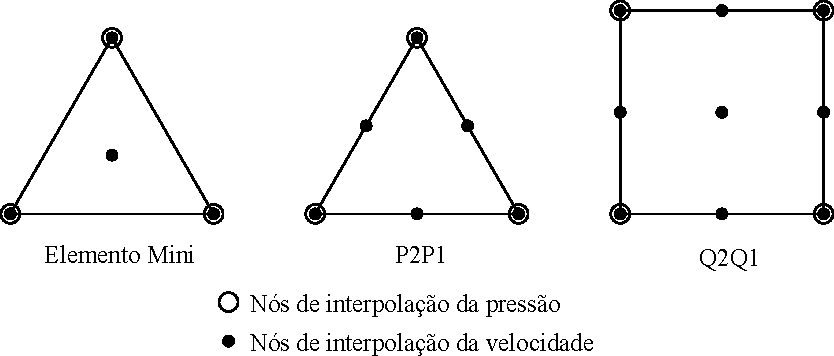
\includegraphics[width=.65\linewidth]{Figuras/Taylor-Hood.pdf}
    \\Fonte: \citeonline{fernandes2020tecnica} - Adaptado.
    \label{fig:Taylor-Hood}
\end{figure}

Uma alternativa ao uso de Elementos Taylor-Hood, e que torna os métodos mais flexíveis, é o emprego de formulações estabilizadas, como a técnica PSPG.

Outra formulação que é eficiente tanto para a estabilização da convecção quanto do campo de pressão, englobando os mesmos termos da estabilização SUPG/PSPG e ainda introduzindo outros termos estabilizantes de forma consistente, é a formulação VMS \cite{bazilevs2013computational}.

%==================================================================================================
\section{\textit{Variational Multi-Scale}} \label{VMS}
%==================================================================================================

O Método Variacional Multiescala, introduzido por \citeonline{hughes1995multiscale,hughes1998variational,hughes2000large}, é um modelo de estabilização multiescala o qual faz a separação dos espaços de tentativas e de testes em subespaços que representem as escalas grosseiras, que se tratam de subespaços de dimensões finitas e denotadas por uma barra, e as escalas finas, que são subespaços de infinitas dimensões e denotadas por $'$, ou seja:

\begin{subequations}
    \begin{align}
         & \script{S}_u=\bar{\script{S}}_u\oplus\script{S}'_u\text{,}  \\
         & \script{S}_p=\bar{\script{S}}_p\oplus\script{S}'_p\text{,}  \\
         & \script{V}_u=\bar{\script{V}}_u\oplus\script{V}'_u\text{ e} \\
         & \script{V}_p=\bar{\script{V}}_p\oplus\script{V}'_p\text{.}
    \end{align}
\end{subequations}

Inicialmente será abordado uma técnica baseada em uma descrição Euleriana com domínio fixo, para maior familiarização com o método, e na sequência será apresentada uma formulação em descrição ALE utilizando domínio móvel.

O sistema a ser resolvido parte do apresentado em \ref{eq:NS-Euler}, que em sua forma fraca se encontra em \ref{eq:WeakForm2}. Primeiramente realiza-se a separação dos membros em:

\begin{subequations}
    \begin{align}
         & u_i=\bar{u}_i+u'_i\text{,}  \\
         & p=\bar{p}+p'\text{,}        \\
         & w_i=\bar{w}_i+w'_i\text{ e} \\
         & q=\bar{q}+q'\text{,}
    \end{align}
\end{subequations}

\noindent em que se adota $w_i=\bar{w}_i$ e $q=\bar{q}$ e as escalas finas $u'_i$ e $p'$ podem ser modeladas como:

\begin{subequations}
    \begin{equation}
        \BB{u}'=-\frac{\tau_{\sups}}{\rho}\rM\text{ e}
    \end{equation}
    \begin{equation}
        p'=-\rho\nu_{\lsic}\rC\text{,}
    \end{equation}
\end{subequations}

\noindent nas quais $\tau_{\sups}$ e $\nu_{\lsic}$ são termos estabilizadores, dados por \cite{bazilevs2013computational}:
%página 80 do pdf de hughes2013 e 65 de fernandes2020

\begin{subequations}
    \begin{equation}
        \tau_{\sups}=\bigpar{\frac{4}{\Delta t^2}+\BBB{u}\cdot\BB{G}\BBB{u}+C_I\nu^2\BB{G}:\BB{G}}^{-1/2}\text{ e}
    \end{equation}
    \begin{equation}
        \nu_{\lsic}=(\tr{\BB{G}}\tau_{\sups})^{-1}\text{,}
    \end{equation}
    \label{eq:TermEstab}
\end{subequations}

\noindent onde $C_I$ é uma constante e:

\begin{equation}
    \BB{G}=\frac{\partial\BB{\xi}}{\partial\BB{y}}^T\frac{\partial\BB{\xi}}{\partial\BB{y}}\text{.}
\end{equation}

Já os termos $\rMi{i}$ e $\rCi$ são os resíduos associados à equação de conservação da quantidade de movimento e da continuidade, respectivamente:

\begin{subequations}
    \begin{equation}
        \rMi{i}=\rho\bigpar{\dot{\bar{u}}_i+\bar{u}_j\bar{u}_{i,j}-\bar{f}_i}-\sigma_{ji,j}\text{ e}
    \end{equation}
    \begin{equation}
        \rCi=\bar{u}_{i,i}\text{.}
    \end{equation}
\end{subequations}

Outra forma de se modelar os termos estabilizadores pode ser dado por \cite{bazilevs2013computational}:

\begin{subequations}
    \begin{equation}
        \tau_{\sups}=\bigpar{\frac{1}{\tau_{\sugn 1}^2}+\frac{1}{\tau_{\sugn 2}^2}+\frac{1}{\tau_{\sugn 3}^2}}^{-1/2}\text{ e}
    \end{equation}
    \begin{equation}
        \nu_{\lsic}=\tau_{\sups}\norm{\BBB{u}}^2\text{,}
    \end{equation}
\end{subequations}

\noindent tal que:

\begin{subequations}
    \begin{align}
         & \tau_{\sugn 1}=\bigpar{\sum_{a=1}^{n_{en}}{\abs{\BBB{u}\cdot\NN N_a}}}^{-1}\text{,} \\
         & \tau_{\sugn 2}=\frac{\Delta t}{2}\text{,}                                           \\
         & \tau_{\sugn 3}=\frac{h_{\rgn}^2}{4\nu}\text{,}                                      \\
         & h_\rgn=2\bigpar{\sum_{a=1}^{n_{en}}{\abs{\BB{r}\cdot\NN N_a}}}^{-1}\text{ e}        \\
         & \BB{r}=\frac{\NN\norm{\BBB{u}}}{\norm{\NN\norm{\BBB{u}}}}\text{.}
    \end{align}
\end{subequations}

Assim, obtém-se o problema do Método Variacional Multiescala Baseado em Resíduos (\textit{Residual-Based Variational Multi-Scale} - RBVMS) que busca determinar $\BBB{u}\in\bar{\script{S}}_u$ e $\bar{p}\in\bar{\script{S}}_p$, tais que para todo $\BBB{w}\in\bar{\script{V}}_u$ e $\bar{q}\in\bar{\script{V}}_p$ \cite{bazilevs2013computational}:

\begin{equation}
    \begin{split}
        &\intDom{\bar{w}_i\rho\bigpar{\dot{\bar{u}}_i+\bar{u}_j\bar{u}_{i,j}-\bar{f}_i}}+\intDom{\bar{w}_{i,j}\bar{\sigma}_{ij}}-\intNeumann{\bar{w}_i\bar{h}_i}+\intDom{\bar{q}\bar{u}_{i,i}}-\\
        &\SintDom{\rho\bigpar{\bar{u}_j\bar{w}_{i,j}+\frac{\bar{q}_{,i}}{\rho}}u'_i}-\SintDom{\bar{w}_{i,i}p'}+\\
        &\SintDom{\rho\bar{w}_iu'_j\bar{u}_{i,j}}-\SintDom{\rho\bar{w}_{i,j}u'_iu'_j}=0
        \text{.}
        \label{eq:RBVMS1}
    \end{split}
\end{equation}

Para a discretização do problema pode-se realizar a separação da dependência espacial e temporal para os espaços tentativas e testes como:

\begin{subequations}
    \begin{align}
         & \bar{u}_i(\BB{y},t)=\sum_{\BB{\eta}^s}{U_i^a(t)N_a(\BB{y})}\text{,}             \\
         & \bar{p}(\BB{y},t)=\sum_{\BB{\eta}^s}{P^a(t)N_a(\BB{y})}\text{,}                 \\
         & \bar{w}_i(\BB{y})=\sum_{\BB{\eta}^w}{W_i^aN_a(\BB{y})}\text{ e}\label{eq:w-sep} \\
         & \bar{q}(\BB{y})=\sum_{\BB{\eta}^w}{Q^aN_a(\BB{y})}\text{.}\label{eq:q-sep}
    \end{align}
\end{subequations}

Substituindo \ref{eq:w-sep} e \ref{eq:q-sep} em \ref{eq:RBVMS1}, tais que $W^a$ e $Q^a$ são valores arbitrários, obtém-se dois vetores ($\NM=[(N_\mathrm{M})_i^a]$ e $\NC=[(N_\mathrm{C})^a]$) que representam resíduos a serem minimizados:

\begin{subequations}
    \begin{equation}
        \begin{split}
            (N_\mathrm{M})_i^a=&
            \intDom{N_a\rho\bigpar{\dot{\bar{u}}_i+\bar{u}_j\bar{u}_{i,j}-\bar{f}_i}}+\intDom{N_{a,j}\bar{\sigma}_{ij}}-\intNeumann{N_a\bar{h}_i}-\\
            &\SintDom{\rho N_{a,j}\bar{u}_ju'_i}-\SintDom{N_{a,i}p'}+\\
            &\SintDom{\rho N_a\bar{u}_{i,j}u'_j}-\SintDom{\rho N_{a,j}u'_iu'_j}
            \text{,}
        \end{split}
    \end{equation}
    \begin{equation}
        (N_\mathrm{C})^a=\intDom{N_a\bar{u}_{i,i}}-\SintDom{N_{a,i}u'_i}
    \end{equation}
    \label{Eq:Residuos-Euler}
\end{subequations}

Sendo os vetores $\BB{U}=[\BB{u}_B]$, $\dot{\BB{U}}=[\dot{\BB{u}}_B]$ e $\BB{P}=[p_B]$, que representam, respectivamente, os graus de liberdade em velocidades, primeira derivada temporal das velocidades e pressões nodais, então o problema a ser resolvido será dado por: encontrar $\BB{U}$, $\dot{\BB{U}}$ e $\BB{P}$, tais que:

\begin{subequations}
    \begin{align}
         & \NM(\BB{U},\dot{\BB{U}},\BB{P})=\BB{0}\text{ e} \\
         & \NC(\BB{U},\dot{\BB{U}},\BB{P})=\BB{0}\text{.}
    \end{align}
\end{subequations}

Uma formulação alternativa à apresentada é apresentada por \citeonline{bazilevs2013computational}, denominada como SUPG/PSPG, onde se omite os dois últimos termos da equação \ref{eq:RBVMS1} e se utiliza de valores diferentes de $\tau$ para as equações de conservação da quantidade de movimento e da continuidade, resultando em:

\begin{equation}
    \begin{split}
        &\intDom{\bar{w}_i\rho\bigpar{\dot{\bar{u}}_i+\bar{u}_j\bar{u}_{i,j}-\bar{f}_i}}+\intDom{\bar{w}_{i,j}\bar{\sigma}_{ij}}-\intNeumann{\bar{w}_i\bar{h}_i}+\intDom{\bar{q}\bar{u}_{i,i}}-\\
        &\SintDom{\tau_\supg\bar{w}_{i,j}\bar{u}_j\rMi{i}}-\SintDom{\tau_\pspg\frac{q_{,i}}{\rho}\rMi{i}}-\\
        &\SintDom{\rho\nu_\lsic\bar{w}_{i,i}\rCi}=0
        \text{,}
        \label{eq:SUPG-PSPG}
    \end{split}
\end{equation}

\noindent na qual, segundo os autores, adota-se $\tau_\pspg=\tau_\supg=\tau_\sups$ para uma boa variedade de problemas.

Por sua vez, a formulação baseada em uma descrição ALE parte das equações apresentadas em \ref{eq:NS-ALE}, cujo problema semi-discreto pode ser dado por:

\begin{equation}
    \begin{split}
        &\intDom{w_i\rho\bigpar{\dot{u}_i+(u_j-\hat{u}_j)u_{i,j}-f_j}}+\intDom{w_{i,j}\sigma_{ij}}-\\
        &\intNeumann{w_ih_i}+\intDom{qu_{i,i}}=0
    \end{split}
\end{equation}

Portanto o problema semi-discreto em formulação RBVMS de escoamentos incompressíveis segundo uma descrição ALE será: encontrar $\BBB{u}\in\bar{\script{S}}_u$ e $\bar{p}\in\bar{\script{S}}_p$, tais que para todo $\BBB{w}\in\bar{\script{V}}_u$ e $\bar{q}\in\bar{\script{V}}_p$ \cite{bazilevs2013computational}:

\begin{equation}
    \begin{split}
        &\intDom{\bar{w}_i\rho\bigpar{\dot{\bar{u}}_i+(\bar{u}_j-\hat{u}_j)\bar{u}_{i,j}-\bar{f}_i}}+\intDom{\bar{w}_{i,j}\bar{\sigma}_{ij}}-\intNeumann{\bar{w}_i\bar{h}_i}+\intDom{\bar{q}\bar{u}_{i,i}}-\\
        &\SintDom{\bigpar{\rho(\bar{u}_j-\hat{u}_j)\bar{w}_{i,j}+\bar{q}_{,i}}u'_i}-\SintDom{\bar{w}_{i,i}p'}+\\
        &\SintDom{\rho\bar{w}_i\bar{u}_{i,j}u'_j}-\SintDom{\rho\bar{w}_{i,j}u'_iu'_j}=0
        \text{,}
        \label{eq:RBVMS-ALE}
    \end{split}
\end{equation}

\noindent em que os termos estabilizadores $\tau_\sups$ e $\nu_\lsic$ são alterados das equações \ref{eq:TermEstab}, onde se considera, ao invés da velocidade do fluido $\bar{u}_i$, a velocidade relativa à malha ($\bar{u}_i-\hat{u}_i$), ou seja, $\bar{u}_i\gets\bar{u}_i-\hat{u}_i$.

Para o problema discretizado utiliza-se as seguintes expressões de aproximação dos espaços tentativas e testes:

\begin{subequations}
    \begin{align}
         & \bar{u}_i(\BB{y},t)=\sum_{\BB{\eta}^s}{U_i^a(t)N_a(\BB{y},t)}\text{,} \\
         & \bar{p}(\BB{y},t)=\sum_{\BB{\eta}^s}{P^a(t)N_a(\BB{y},t)}\text{,}     \\
         & \bar{w}_i(\BB{y})=\sum_{\BB{\eta}^w}{W_i^aN_a(\BB{y},t)}\text{ e}     \\
         & \bar{q}(\BB{y})=\sum_{\BB{\eta}^w}{Q^aN_a(\BB{y},t)}\text{,}
    \end{align}
\end{subequations}

\noindent onde as funções de forma $N_a(\BB{y},t)$ são definidas como:

\begin{equation}
    N_a(\BB{y},t)=\hat{N}_a(\bhat{f}^{-1}(\BB{y},t))\text{,}
\end{equation}

\noindent em que $\bhat{f}(\BB{y},t)$ é a função de mudança de configuração de $\hat{\Omega}\to\Omega$, conforme apresentado no item \ref{CFD-ALE}, dada em sua forma discreta por:

\begin{equation}
    \bhat{f}(\bhat{x},t)=\sum_{a\in\BB{\eta}^s}{(\bhat{x}_a+\Delta\bhat{x}_a(t))\hat{N}_a(\bhat{x})}\text{,}
\end{equation}

\noindent sendo $\bhat{x}_a$ as posições nodais em $\hat{\Omega}$, $\Delta\bhat{x}(t)$ o deslocamento nodal e $\hat{N}_a$ é a função de forma fixa da discretização de $\hat{\Omega}$. Nota-se, portanto, que as funções $N_a(\BB{y},t)$ possuem dependência temporal devido à movimentação da malha.

Com isso, define-se os vetores de resíduos da conservação de quantidade de movimento de da continuidade como:

\begin{subequations}
    \begin{equation}
        \NM=[(N_\mathrm{M})_i^a]\text{,}
    \end{equation}
    \begin{equation}
        \NC=[(N_\mathrm{C})^a]\text{,}
    \end{equation}
    \begin{equation}
        \begin{split}
            (N_\mathrm{M})_i^a=&
            \intDom{N_a\rho\bigpar{\dot{\bar{u}}_i+(\bar{u}_j-\hat{u}_j)\bar{u}_{i,j}-\bar{f}_i}}+\intDom{N_{a,j}\bar{\sigma}_{ij}}-\intNeumann{N_a\bar{h}_i}-\\
            &\SintDom{\rho N_{a,j}(\bar{u}_j-\hat{u}_j)u'_i}-\SintDom{N_{a,i}p'}+\\
            &\SintDom{\rho N_a\bar{u}_{i,j}u'_j}-\SintDom{\rho N_{a,j}u'_iu'_j}
            \text{,}
        \end{split}
    \end{equation}
    \begin{equation}
        (N_\mathrm{C})^a=\intDom{N_a\bar{u}_{i,i}}-\SintDom{N_{a,i}u'_i}
    \end{equation}
    \label{Eq:Residuos-ALE}
\end{subequations}

Assim, pretende-se determinar os vetores $\BB{U}$, $\dot{\BB{U}}$ e $\BB{P}$, tais que:

\begin{subequations}
    \begin{align}
         & \NM(\BB{U},\dot{\BB{U}},\BB{P})=\BB{0}\text{ e} \\
         & \NC(\BB{U},\dot{\BB{U}},\BB{P})=\BB{0}\text{.}
    \end{align}
\end{subequations}

%==================================================================================================
\subsection{Integração temporal} \label{IT-VMS}
%==================================================================================================

Como pôde-se verificar, em ambas as descrições, Euleriana e ALE, chega-se a um problema discreto no espaço, porém contínuo no tempo (Equações \ref{Eq:Residuos-Euler} e \ref{Eq:Residuos-ALE}). Dessa forma torna-se necessária a devida discretização temporal das variáveis, que pode ocorrer de diferentes formas, como apontado por \citeonline{reddy2010finite}, tem-se, por exemplo, o surgimento de integradores explícitos, como o integrador baseado em diferenças adiantadas, implícitos, como em diferenças finitas atrasadas, e o denominado semi-explícito (ou da regra de trapézios). Segundo o autor os integradores implícitos possuem vantagens sobre os explícitos, uma vez que: se observa a implicidade natural da pressão em escoamentos incompressíveis; deve-se ter um cuidado extra para garantir a estabilidade do integrador; apresentar problemas para a diagonalização de matrizes de massa; e perda de precisão na diagonalização.

O integrador temporal utilizado no presente trabalho é o denominado integrador $\alpha$-generalizado, desenvolvido por \citeonline{chung1993time}, que possui a capacidade de representar adequadamente problema de escoamentos incompressíveis, além de permitir a introdução de difusão numérica ao processo \cite{fernandes2020tecnica}.

Esse integrador parte da consideração de valores intermediários de aceleração e velocidade em um intervalo de tempo $[t_n,t_{n+1}]$ no $n$-ésimo passo de tempo, representados respectivamente por $\dot{\BB{U}}^{n+\alpha_m}$ e $\BB{U}^{n+\alpha_f}$:

\begin{subequations}
    \begin{equation}
        \dot{\BB{U}}^{n+\alpha_m}=\dot{\BB{U}}^n+\alpha_m(\dot{\BB{U}}^{n+1}-\dot{\BB{U}}^n)\text{ e}
    \end{equation}
    \begin{equation}
        \BB{U}^{n+\alpha_f}=\BB{U}^n+\alpha_f(\BB{U}^{n+1}-\BB{U}^n)\text{.}
    \end{equation}
\end{subequations}

Já para se relacionar a velocidade à aceleração, pode-se proceder com a aproximação de Newmark \cite{bazilevs2013computational}:

\begin{equation}
    \BB{U}^{n+1}=\BB{U}^n+\Delta t_n\bigpar{(1-\gamma)\dot{\BB{U}}^n+\gamma\dot{\BB{U}}^{n+1}}\text{,}
\end{equation}

\noindent sendo $\alpha_m$, $\alpha_f$ e $\gamma$ valores escolhidos arbitrariamente observando as necessidades de estabilidade e precisão do método.

De acordo com \citeonline{chung1993time,jansen2000generalized,bazilevs2013computational}, a precisão de segunda ordem dessa aproximação pode ser atingida uma vez que:

\begin{equation}
    \gamma=\frac{1}{2}+\alpha_m-\alpha_f\text{,}
\end{equation}

\noindent enquanto a estabilidade incondicional pode ser obtida caso:

\begin{equation}
    \alpha_m\geq\alpha_f\geq\frac{1}{2}\text{.}
\end{equation}

Ainda é possível escrever, a partir da Equação \ref{eq:one-par-stable}, $\alpha_m$ e $\alpha_f$ em termos de um parâmetro arbitrário único  ($0\leq\rho_\infty\leq1$), que representa o raio espectral de amplificação da matriz para $\Delta t\to\infty$, o qual é utilizado para controlar as dissipações de alta-frequência.

\begin{subequations}
    \begin{equation}
        \alpha_m=\frac{1}{2}\bigpar{\frac{3-\rho_\infty}{1+\rho_\infty}}\text{ e}
    \end{equation}
    \begin{equation}
        \alpha_f=\frac{1}{1+\rho_\infty}\text{.}
    \end{equation}
    \label{eq:one-par-stable}
\end{subequations}

Para o caso de $\rho_\infty=1$ não ocorre a introdução de difusão numérica, enquanto para $\rho_\infty=0$ se tem a máxima dissipação de altas frequências \cite{fernandes2020tecnica}.

Sendo assim, os resíduos obtidos anteriormente podem ser escritos em termos dos valores intermediários como:

\begin{subequations}
    \begin{equation}
        \NM(\dot{\BB{U}}^{n+\alpha_m},\BB{U}^{n+\alpha_f},\BB{P}^{n+1})=0
    \end{equation}
    \begin{equation}
        \NC(\dot{\BB{U}}^{n+\alpha_m},\BB{U}^{n+\alpha_f},\BB{P}^{n+1})=0
    \end{equation}
\end{subequations}

%%==================================================================================================
%\subsection{Procedimento iterativo} \label{Comp-VMS}
%%==================================================================================================
%
%O procedimento para minimizar os vetores resíduo obtido parte do método de Newton-Raphson, no qual os valores a serem corrigidos são os vetores de acelerações nodais ($\dot{\BB{U}}$) e de pressões nodais ($\BB{P}$). Dessa forma, o problema a ser resolvido para a correção dessas variáveis é:
%
%\begin{equation}
%    \begin{bmatrix}
%        \der{(N_M)_i^a}{(\dot{U}_j^b)^{n+1}} & \der{(N_M)_i^a}{(P^b)^{n+1}} \\
%        \der{(N_C)^a}{(\dot{U}_j^b)^{n+1}}   & \der{(N_C)^a}{(P^b)^{n+1}}
%    \end{bmatrix}
%    \begin{bmatrix}
%        \Delta(\dot{U}_j^b)^{n+1} \\
%        \Delta (P^b)^{n+1}
%    \end{bmatrix}=-
%    \begin{bmatrix}
%        (N_M)_i^a \\
%        (N_C)^a
%    \end{bmatrix}\text{,}
%    \label{Eq:Newton-Raphson}
%\end{equation}
%
%\noindent em que, para uma descrição ALE:
%
%\begin{subequations}
%    \begin{equation}
%        \begin{split}
%            \der{(N_M)_i^a}{(\dot{U}_j^b)^{n+1}}=&\am\intDomna{\rho N_aN_b}\dij+\am\intDomna{\rho\tsups N_{a,k}N_{b}\uub{k}}\dij+\\
%            &\agdt\intDomna{\rho N_aN_{b,k}\uub{k}}\dij+\agdt\intDomna{\mu N_{a,k}N_{b,k}}\dij+\\
%            &\agdt\intDomna{\mu N_{a,j}N_{b,i}}+\agdt\intDomna{\rho\nlsic N_{a,i}N_{b,j}}+\\
%            &\agdt\intDomna{\rho\tsups N_{a,k}N_{b,m}\uub{k}\uub{m}}\dij+\\
%            &\agdt\intDomna{\rho N_aN_b\bar{u}_{i,j}}+\agdt\intDomna{\rho\tsups N_{a,k}N_b\uub{k}\bar{u}_{i,j}}-\\
%            &\am\intDomna{\rho\tsups N_aN_b\bar{u}_{i,j}}-\\
%            &\agdt\intDomna{\rho\tsups N_aN_{b,m}\uub{m}\bar{u}_{i,j}}-\\
%            &\agdt\intDomna{\rho\tsups N_aN_b\bar{u}_{i,k}\bar{u}_{k,j}}\text{,}
%        \end{split}
%    \end{equation}
%    \begin{equation}
%        \begin{split}
%            \der{(N_M)_i^a}{(P^b)^{n+1}}=&-\intDomna{N_{a,i}N_b}+\intDomna{\tsups N_{a,j}N_{b,i}\uub{j}}-\\
%            &\intDomna{\tsups N_aN_{b,j}\bar{u}_{i,j}}\text{,}
%        \end{split}
%    \end{equation}
%    \begin{equation}
%        \begin{split}
%            \der{(N_C)^a}{(\dot{U}_j^b)^{n+1}}=&\agdt\intDomna{N_aN_{b,j}}+\am\intDomna{\tsups N_{a,j}N_b}+\\
%            &\agdt\intDomna{\tsups N_{a,j}N_{b,m}\uub{m}}+\\
%            &\agdt\intDomna{\tsups N_{a,i}N_b\bar{u}_{i,j}}\text{ e}
%        \end{split}
%    \end{equation}
%    \begin{equation}
%        \der{(N_C)^a}{(P^b)^{n+1}}=\intDomna{\frac{\tsups}{\rho}N_{a,i}N_{b,i}}\text{,}
%    \end{equation}
%\end{subequations}
%
%\noindent em que $\agdt=\alpha_f\gamma\Delta t$ e:
%
%\begin{equation}
%    \Omega^{n+\alpha_f}=\left\{\bar{\BB{x}}|\bar{\BB{x}}(\hat{\BB{x}},t^{n+\alpha_f})=\alpha_f\bar{\BB{x}}(\hat{\BB{x}},t^{n+1})+(1-\alpha_f)\bar{\BB{x}}(\hat{\BB{x}},t^n)\right\}\text{.}
%\end{equation}
%
%Para uma descrição Euleriana, considera-se a velocidade da malha como nula na formulação apresentada.
%
%Sendo assim, o pseudocódigo apresentado no algoritmo presente no Apêndice \ref{Ap:MEF-VMS} mostra o procedimento para obtenção da solução aproximada.
%==================================================================================================
\section{Modelos de Turbulência} \label{MdT}
%==================================================================================================

A presente seção apresentará a fundamentação teórica dos modelos de turbulência baseado em grandes vórtices (LES) no item \ref{LES} e \textit{Reynolds-Averaged Navier-Stokes} (RANS) no item \ref{RANS}.

%%==================================================================================================
\section{\textit{Variational Multi-Scale}} \label{VMS}
%==================================================================================================

O Método Variacional Multiescala, introduzido por \citeonline{hughes1995multiscale,hughes1998variational,hughes2000large}, é um modelo de estabilização multiescala o qual faz a separação dos espaços de tentativas e de testes em subespaços que representem as escalas grosseiras, que se tratam de subespaços de dimensões finitas e denotadas por uma barra, e as escalas finas, que são subespaços de infinitas dimensões e denotadas por $'$, ou seja:

\begin{subequations}
    \begin{align}
         & \script{S}_u=\bar{\script{S}}_u\oplus\script{S}'_u\text{,}  \\
         & \script{S}_p=\bar{\script{S}}_p\oplus\script{S}'_p\text{,}  \\
         & \script{V}_u=\bar{\script{V}}_u\oplus\script{V}'_u\text{ e} \\
         & \script{V}_p=\bar{\script{V}}_p\oplus\script{V}'_p\text{.}
    \end{align}
\end{subequations}

Inicialmente será abordado uma técnica baseada em uma descrição Euleriana com domínio fixo, para maior familiarização com o método, e na sequência será apresentada uma formulação em descrição ALE utilizando domínio móvel.

O sistema a ser resolvido parte do apresentado em \ref{eq:NS-Euler}, que em sua forma fraca se encontra em \ref{eq:WeakForm2}. Primeiramente realiza-se a separação dos membros em:

\begin{subequations}
    \begin{align}
         & u_i=\bar{u}_i+u'_i\text{,}  \\
         & p=\bar{p}+p'\text{,}        \\
         & w_i=\bar{w}_i+w'_i\text{ e} \\
         & q=\bar{q}+q'\text{,}
    \end{align}
\end{subequations}

\noindent em que se adota $w_i=\bar{w}_i$ e $q=\bar{q}$ e as escalas finas $u'_i$ e $p'$ podem ser modeladas como:

\begin{subequations}
    \begin{equation}
        \BB{u}'=-\frac{\tau_{\sups}}{\rho}\rM\text{ e}
    \end{equation}
    \begin{equation}
        p'=-\rho\nu_{\lsic}\rC\text{,}
    \end{equation}
\end{subequations}

\noindent nas quais $\tau_{\sups}$ e $\nu_{\lsic}$ são termos estabilizadores, dados por \cite{bazilevs2013computational}:
%página 80 do pdf de hughes2013 e 65 de fernandes2020

\begin{subequations}
    \begin{equation}
        \tau_{\sups}=\bigpar{\frac{4}{\Delta t^2}+\BBB{u}\cdot\BB{G}\BBB{u}+C_I\nu^2\BB{G}:\BB{G}}^{-1/2}\text{ e}
    \end{equation}
    \begin{equation}
        \nu_{\lsic}=(\tr{\BB{G}}\tau_{\sups})^{-1}\text{,}
    \end{equation}
    \label{eq:TermEstab}
\end{subequations}

\noindent onde $C_I$ é uma constante e:

\begin{equation}
    \BB{G}=\frac{\partial\BB{\xi}}{\partial\BB{y}}^T\frac{\partial\BB{\xi}}{\partial\BB{y}}\text{.}
\end{equation}

Já os termos $\rMi{i}$ e $\rCi$ são os resíduos associados à equação de conservação da quantidade de movimento e da continuidade, respectivamente:

\begin{subequations}
    \begin{equation}
        \rMi{i}=\rho\bigpar{\dot{\bar{u}}_i+\bar{u}_j\bar{u}_{i,j}-\bar{f}_i}-\sigma_{ji,j}\text{ e}
    \end{equation}
    \begin{equation}
        \rCi=\bar{u}_{i,i}\text{.}
    \end{equation}
\end{subequations}

Outra forma de se modelar os termos estabilizadores pode ser dado por \cite{bazilevs2013computational}:

\begin{subequations}
    \begin{equation}
        \tau_{\sups}=\bigpar{\frac{1}{\tau_{\sugn 1}^2}+\frac{1}{\tau_{\sugn 2}^2}+\frac{1}{\tau_{\sugn 3}^2}}^{-1/2}\text{ e}
    \end{equation}
    \begin{equation}
        \nu_{\lsic}=\tau_{\sups}\norm{\BBB{u}}^2\text{,}
    \end{equation}
\end{subequations}

\noindent tal que:

\begin{subequations}
    \begin{align}
         & \tau_{\sugn 1}=\bigpar{\sum_{a=1}^{n_{en}}{\abs{\BBB{u}\cdot\NN N_a}}}^{-1}\text{,} \\
         & \tau_{\sugn 2}=\frac{\Delta t}{2}\text{,}                                           \\
         & \tau_{\sugn 3}=\frac{h_{\rgn}^2}{4\nu}\text{,}                                      \\
         & h_\rgn=2\bigpar{\sum_{a=1}^{n_{en}}{\abs{\BB{r}\cdot\NN N_a}}}^{-1}\text{ e}        \\
         & \BB{r}=\frac{\NN\norm{\BBB{u}}}{\norm{\NN\norm{\BBB{u}}}}\text{.}
    \end{align}
\end{subequations}

Assim, obtém-se o problema do Método Variacional Multiescala Baseado em Resíduos (\textit{Residual-Based Variational Multi-Scale} - RBVMS) que busca determinar $\BBB{u}\in\bar{\script{S}}_u$ e $\bar{p}\in\bar{\script{S}}_p$, tais que para todo $\BBB{w}\in\bar{\script{V}}_u$ e $\bar{q}\in\bar{\script{V}}_p$ \cite{bazilevs2013computational}:

\begin{equation}
    \begin{split}
        &\intDom{\bar{w}_i\rho\bigpar{\dot{\bar{u}}_i+\bar{u}_j\bar{u}_{i,j}-\bar{f}_i}}+\intDom{\bar{w}_{i,j}\bar{\sigma}_{ij}}-\intNeumann{\bar{w}_i\bar{h}_i}+\intDom{\bar{q}\bar{u}_{i,i}}-\\
        &\SintDom{\rho\bigpar{\bar{u}_j\bar{w}_{i,j}+\frac{\bar{q}_{,i}}{\rho}}u'_i}-\SintDom{\bar{w}_{i,i}p'}+\\
        &\SintDom{\rho\bar{w}_iu'_j\bar{u}_{i,j}}-\SintDom{\rho\bar{w}_{i,j}u'_iu'_j}=0
        \text{.}
        \label{eq:RBVMS1}
    \end{split}
\end{equation}

Para a discretização do problema pode-se realizar a separação da dependência espacial e temporal para os espaços tentativas e testes como:

\begin{subequations}
    \begin{align}
         & \bar{u}_i(\BB{y},t)=\sum_{\BB{\eta}^s}{U_i^a(t)N_a(\BB{y})}\text{,}             \\
         & \bar{p}(\BB{y},t)=\sum_{\BB{\eta}^s}{P^a(t)N_a(\BB{y})}\text{,}                 \\
         & \bar{w}_i(\BB{y})=\sum_{\BB{\eta}^w}{W_i^aN_a(\BB{y})}\text{ e}\label{eq:w-sep} \\
         & \bar{q}(\BB{y})=\sum_{\BB{\eta}^w}{Q^aN_a(\BB{y})}\text{.}\label{eq:q-sep}
    \end{align}
\end{subequations}

Substituindo \ref{eq:w-sep} e \ref{eq:q-sep} em \ref{eq:RBVMS1}, tais que $W^a$ e $Q^a$ são valores arbitrários, obtém-se dois vetores ($\NM=[(N_\mathrm{M})_i^a]$ e $\NC=[(N_\mathrm{C})^a]$) que representam resíduos a serem minimizados:

\begin{subequations}
    \begin{equation}
        \begin{split}
            (N_\mathrm{M})_i^a=&
            \intDom{N_a\rho\bigpar{\dot{\bar{u}}_i+\bar{u}_j\bar{u}_{i,j}-\bar{f}_i}}+\intDom{N_{a,j}\bar{\sigma}_{ij}}-\intNeumann{N_a\bar{h}_i}-\\
            &\SintDom{\rho N_{a,j}\bar{u}_ju'_i}-\SintDom{N_{a,i}p'}+\\
            &\SintDom{\rho N_a\bar{u}_{i,j}u'_j}-\SintDom{\rho N_{a,j}u'_iu'_j}
            \text{,}
        \end{split}
    \end{equation}
    \begin{equation}
        (N_\mathrm{C})^a=\intDom{N_a\bar{u}_{i,i}}-\SintDom{N_{a,i}u'_i}
    \end{equation}
    \label{Eq:Residuos-Euler}
\end{subequations}

Sendo os vetores $\BB{U}=[\BB{u}_B]$, $\dot{\BB{U}}=[\dot{\BB{u}}_B]$ e $\BB{P}=[p_B]$, que representam, respectivamente, os graus de liberdade em velocidades, primeira derivada temporal das velocidades e pressões nodais, então o problema a ser resolvido será dado por: encontrar $\BB{U}$, $\dot{\BB{U}}$ e $\BB{P}$, tais que:

\begin{subequations}
    \begin{align}
         & \NM(\BB{U},\dot{\BB{U}},\BB{P})=\BB{0}\text{ e} \\
         & \NC(\BB{U},\dot{\BB{U}},\BB{P})=\BB{0}\text{.}
    \end{align}
\end{subequations}

Uma formulação alternativa à apresentada é apresentada por \citeonline{bazilevs2013computational}, denominada como SUPG/PSPG, onde se omite os dois últimos termos da equação \ref{eq:RBVMS1} e se utiliza de valores diferentes de $\tau$ para as equações de conservação da quantidade de movimento e da continuidade, resultando em:

\begin{equation}
    \begin{split}
        &\intDom{\bar{w}_i\rho\bigpar{\dot{\bar{u}}_i+\bar{u}_j\bar{u}_{i,j}-\bar{f}_i}}+\intDom{\bar{w}_{i,j}\bar{\sigma}_{ij}}-\intNeumann{\bar{w}_i\bar{h}_i}+\intDom{\bar{q}\bar{u}_{i,i}}-\\
        &\SintDom{\tau_\supg\bar{w}_{i,j}\bar{u}_j\rMi{i}}-\SintDom{\tau_\pspg\frac{q_{,i}}{\rho}\rMi{i}}-\\
        &\SintDom{\rho\nu_\lsic\bar{w}_{i,i}\rCi}=0
        \text{,}
        \label{eq:SUPG-PSPG}
    \end{split}
\end{equation}

\noindent na qual, segundo os autores, adota-se $\tau_\pspg=\tau_\supg=\tau_\sups$ para uma boa variedade de problemas.

Por sua vez, a formulação baseada em uma descrição ALE parte das equações apresentadas em \ref{eq:NS-ALE}, cujo problema semi-discreto pode ser dado por:

\begin{equation}
    \begin{split}
        &\intDom{w_i\rho\bigpar{\dot{u}_i+(u_j-\hat{u}_j)u_{i,j}-f_j}}+\intDom{w_{i,j}\sigma_{ij}}-\\
        &\intNeumann{w_ih_i}+\intDom{qu_{i,i}}=0
    \end{split}
\end{equation}

Portanto o problema semi-discreto em formulação RBVMS de escoamentos incompressíveis segundo uma descrição ALE será: encontrar $\BBB{u}\in\bar{\script{S}}_u$ e $\bar{p}\in\bar{\script{S}}_p$, tais que para todo $\BBB{w}\in\bar{\script{V}}_u$ e $\bar{q}\in\bar{\script{V}}_p$ \cite{bazilevs2013computational}:

\begin{equation}
    \begin{split}
        &\intDom{\bar{w}_i\rho\bigpar{\dot{\bar{u}}_i+(\bar{u}_j-\hat{u}_j)\bar{u}_{i,j}-\bar{f}_i}}+\intDom{\bar{w}_{i,j}\bar{\sigma}_{ij}}-\intNeumann{\bar{w}_i\bar{h}_i}+\intDom{\bar{q}\bar{u}_{i,i}}-\\
        &\SintDom{\bigpar{\rho(\bar{u}_j-\hat{u}_j)\bar{w}_{i,j}+\bar{q}_{,i}}u'_i}-\SintDom{\bar{w}_{i,i}p'}+\\
        &\SintDom{\rho\bar{w}_i\bar{u}_{i,j}u'_j}-\SintDom{\rho\bar{w}_{i,j}u'_iu'_j}=0
        \text{,}
        \label{eq:RBVMS-ALE}
    \end{split}
\end{equation}

\noindent em que os termos estabilizadores $\tau_\sups$ e $\nu_\lsic$ são alterados das equações \ref{eq:TermEstab}, onde se considera, ao invés da velocidade do fluido $\bar{u}_i$, a velocidade relativa à malha ($\bar{u}_i-\hat{u}_i$), ou seja, $\bar{u}_i\gets\bar{u}_i-\hat{u}_i$.

Para o problema discretizado utiliza-se as seguintes expressões de aproximação dos espaços tentativas e testes:

\begin{subequations}
    \begin{align}
         & \bar{u}_i(\BB{y},t)=\sum_{\BB{\eta}^s}{U_i^a(t)N_a(\BB{y},t)}\text{,} \\
         & \bar{p}(\BB{y},t)=\sum_{\BB{\eta}^s}{P^a(t)N_a(\BB{y},t)}\text{,}     \\
         & \bar{w}_i(\BB{y})=\sum_{\BB{\eta}^w}{W_i^aN_a(\BB{y},t)}\text{ e}     \\
         & \bar{q}(\BB{y})=\sum_{\BB{\eta}^w}{Q^aN_a(\BB{y},t)}\text{,}
    \end{align}
\end{subequations}

\noindent onde as funções de forma $N_a(\BB{y},t)$ são definidas como:

\begin{equation}
    N_a(\BB{y},t)=\hat{N}_a(\bhat{f}^{-1}(\BB{y},t))\text{,}
\end{equation}

\noindent em que $\bhat{f}(\BB{y},t)$ é a função de mudança de configuração de $\hat{\Omega}\to\Omega$, conforme apresentado no item \ref{CFD-ALE}, dada em sua forma discreta por:

\begin{equation}
    \bhat{f}(\bhat{x},t)=\sum_{a\in\BB{\eta}^s}{(\bhat{x}_a+\Delta\bhat{x}_a(t))\hat{N}_a(\bhat{x})}\text{,}
\end{equation}

\noindent sendo $\bhat{x}_a$ as posições nodais em $\hat{\Omega}$, $\Delta\bhat{x}(t)$ o deslocamento nodal e $\hat{N}_a$ é a função de forma fixa da discretização de $\hat{\Omega}$. Nota-se, portanto, que as funções $N_a(\BB{y},t)$ possuem dependência temporal devido à movimentação da malha.

Com isso, define-se os vetores de resíduos da conservação de quantidade de movimento de da continuidade como:

\begin{subequations}
    \begin{equation}
        \NM=[(N_\mathrm{M})_i^a]\text{,}
    \end{equation}
    \begin{equation}
        \NC=[(N_\mathrm{C})^a]\text{,}
    \end{equation}
    \begin{equation}
        \begin{split}
            (N_\mathrm{M})_i^a=&
            \intDom{N_a\rho\bigpar{\dot{\bar{u}}_i+(\bar{u}_j-\hat{u}_j)\bar{u}_{i,j}-\bar{f}_i}}+\intDom{N_{a,j}\bar{\sigma}_{ij}}-\intNeumann{N_a\bar{h}_i}-\\
            &\SintDom{\rho N_{a,j}(\bar{u}_j-\hat{u}_j)u'_i}-\SintDom{N_{a,i}p'}+\\
            &\SintDom{\rho N_a\bar{u}_{i,j}u'_j}-\SintDom{\rho N_{a,j}u'_iu'_j}
            \text{,}
        \end{split}
    \end{equation}
    \begin{equation}
        (N_\mathrm{C})^a=\intDom{N_a\bar{u}_{i,i}}-\SintDom{N_{a,i}u'_i}
    \end{equation}
    \label{Eq:Residuos-ALE}
\end{subequations}

Assim, pretende-se determinar os vetores $\BB{U}$, $\dot{\BB{U}}$ e $\BB{P}$, tais que:

\begin{subequations}
    \begin{align}
         & \NM(\BB{U},\dot{\BB{U}},\BB{P})=\BB{0}\text{ e} \\
         & \NC(\BB{U},\dot{\BB{U}},\BB{P})=\BB{0}\text{.}
    \end{align}
\end{subequations}

%==================================================================================================
\subsection{Integração temporal} \label{IT-VMS}
%==================================================================================================

Como pôde-se verificar, em ambas as descrições, Euleriana e ALE, chega-se a um problema discreto no espaço, porém contínuo no tempo (Equações \ref{Eq:Residuos-Euler} e \ref{Eq:Residuos-ALE}). Dessa forma torna-se necessária a devida discretização temporal das variáveis, que pode ocorrer de diferentes formas, como apontado por \citeonline{reddy2010finite}, tem-se, por exemplo, o surgimento de integradores explícitos, como o integrador baseado em diferenças adiantadas, implícitos, como em diferenças finitas atrasadas, e o denominado semi-explícito (ou da regra de trapézios). Segundo o autor os integradores implícitos possuem vantagens sobre os explícitos, uma vez que: se observa a implicidade natural da pressão em escoamentos incompressíveis; deve-se ter um cuidado extra para garantir a estabilidade do integrador; apresentar problemas para a diagonalização de matrizes de massa; e perda de precisão na diagonalização.

O integrador temporal utilizado no presente trabalho é o denominado integrador $\alpha$-generalizado, desenvolvido por \citeonline{chung1993time}, que possui a capacidade de representar adequadamente problema de escoamentos incompressíveis, além de permitir a introdução de difusão numérica ao processo \cite{fernandes2020tecnica}.

Esse integrador parte da consideração de valores intermediários de aceleração e velocidade em um intervalo de tempo $[t_n,t_{n+1}]$ no $n$-ésimo passo de tempo, representados respectivamente por $\dot{\BB{U}}^{n+\alpha_m}$ e $\BB{U}^{n+\alpha_f}$:

\begin{subequations}
    \begin{equation}
        \dot{\BB{U}}^{n+\alpha_m}=\dot{\BB{U}}^n+\alpha_m(\dot{\BB{U}}^{n+1}-\dot{\BB{U}}^n)\text{ e}
    \end{equation}
    \begin{equation}
        \BB{U}^{n+\alpha_f}=\BB{U}^n+\alpha_f(\BB{U}^{n+1}-\BB{U}^n)\text{.}
    \end{equation}
\end{subequations}

Já para se relacionar a velocidade à aceleração, pode-se proceder com a aproximação de Newmark \cite{bazilevs2013computational}:

\begin{equation}
    \BB{U}^{n+1}=\BB{U}^n+\Delta t_n\bigpar{(1-\gamma)\dot{\BB{U}}^n+\gamma\dot{\BB{U}}^{n+1}}\text{,}
\end{equation}

\noindent sendo $\alpha_m$, $\alpha_f$ e $\gamma$ valores escolhidos arbitrariamente observando as necessidades de estabilidade e precisão do método.

De acordo com \citeonline{chung1993time,jansen2000generalized,bazilevs2013computational}, a precisão de segunda ordem dessa aproximação pode ser atingida uma vez que:

\begin{equation}
    \gamma=\frac{1}{2}+\alpha_m-\alpha_f\text{,}
\end{equation}

\noindent enquanto a estabilidade incondicional pode ser obtida caso:

\begin{equation}
    \alpha_m\geq\alpha_f\geq\frac{1}{2}\text{.}
\end{equation}

Ainda é possível escrever, a partir da Equação \ref{eq:one-par-stable}, $\alpha_m$ e $\alpha_f$ em termos de um parâmetro arbitrário único  ($0\leq\rho_\infty\leq1$), que representa o raio espectral de amplificação da matriz para $\Delta t\to\infty$, o qual é utilizado para controlar as dissipações de alta-frequência.

\begin{subequations}
    \begin{equation}
        \alpha_m=\frac{1}{2}\bigpar{\frac{3-\rho_\infty}{1+\rho_\infty}}\text{ e}
    \end{equation}
    \begin{equation}
        \alpha_f=\frac{1}{1+\rho_\infty}\text{.}
    \end{equation}
    \label{eq:one-par-stable}
\end{subequations}

Para o caso de $\rho_\infty=1$ não ocorre a introdução de difusão numérica, enquanto para $\rho_\infty=0$ se tem a máxima dissipação de altas frequências \cite{fernandes2020tecnica}.

Sendo assim, os resíduos obtidos anteriormente podem ser escritos em termos dos valores intermediários como:

\begin{subequations}
    \begin{equation}
        \NM(\dot{\BB{U}}^{n+\alpha_m},\BB{U}^{n+\alpha_f},\BB{P}^{n+1})=0
    \end{equation}
    \begin{equation}
        \NC(\dot{\BB{U}}^{n+\alpha_m},\BB{U}^{n+\alpha_f},\BB{P}^{n+1})=0
    \end{equation}
\end{subequations}

%%==================================================================================================
%\subsection{Procedimento iterativo} \label{Comp-VMS}
%%==================================================================================================
%
%O procedimento para minimizar os vetores resíduo obtido parte do método de Newton-Raphson, no qual os valores a serem corrigidos são os vetores de acelerações nodais ($\dot{\BB{U}}$) e de pressões nodais ($\BB{P}$). Dessa forma, o problema a ser resolvido para a correção dessas variáveis é:
%
%\begin{equation}
%    \begin{bmatrix}
%        \der{(N_M)_i^a}{(\dot{U}_j^b)^{n+1}} & \der{(N_M)_i^a}{(P^b)^{n+1}} \\
%        \der{(N_C)^a}{(\dot{U}_j^b)^{n+1}}   & \der{(N_C)^a}{(P^b)^{n+1}}
%    \end{bmatrix}
%    \begin{bmatrix}
%        \Delta(\dot{U}_j^b)^{n+1} \\
%        \Delta (P^b)^{n+1}
%    \end{bmatrix}=-
%    \begin{bmatrix}
%        (N_M)_i^a \\
%        (N_C)^a
%    \end{bmatrix}\text{,}
%    \label{Eq:Newton-Raphson}
%\end{equation}
%
%\noindent em que, para uma descrição ALE:
%
%\begin{subequations}
%    \begin{equation}
%        \begin{split}
%            \der{(N_M)_i^a}{(\dot{U}_j^b)^{n+1}}=&\am\intDomna{\rho N_aN_b}\dij+\am\intDomna{\rho\tsups N_{a,k}N_{b}\uub{k}}\dij+\\
%            &\agdt\intDomna{\rho N_aN_{b,k}\uub{k}}\dij+\agdt\intDomna{\mu N_{a,k}N_{b,k}}\dij+\\
%            &\agdt\intDomna{\mu N_{a,j}N_{b,i}}+\agdt\intDomna{\rho\nlsic N_{a,i}N_{b,j}}+\\
%            &\agdt\intDomna{\rho\tsups N_{a,k}N_{b,m}\uub{k}\uub{m}}\dij+\\
%            &\agdt\intDomna{\rho N_aN_b\bar{u}_{i,j}}+\agdt\intDomna{\rho\tsups N_{a,k}N_b\uub{k}\bar{u}_{i,j}}-\\
%            &\am\intDomna{\rho\tsups N_aN_b\bar{u}_{i,j}}-\\
%            &\agdt\intDomna{\rho\tsups N_aN_{b,m}\uub{m}\bar{u}_{i,j}}-\\
%            &\agdt\intDomna{\rho\tsups N_aN_b\bar{u}_{i,k}\bar{u}_{k,j}}\text{,}
%        \end{split}
%    \end{equation}
%    \begin{equation}
%        \begin{split}
%            \der{(N_M)_i^a}{(P^b)^{n+1}}=&-\intDomna{N_{a,i}N_b}+\intDomna{\tsups N_{a,j}N_{b,i}\uub{j}}-\\
%            &\intDomna{\tsups N_aN_{b,j}\bar{u}_{i,j}}\text{,}
%        \end{split}
%    \end{equation}
%    \begin{equation}
%        \begin{split}
%            \der{(N_C)^a}{(\dot{U}_j^b)^{n+1}}=&\agdt\intDomna{N_aN_{b,j}}+\am\intDomna{\tsups N_{a,j}N_b}+\\
%            &\agdt\intDomna{\tsups N_{a,j}N_{b,m}\uub{m}}+\\
%            &\agdt\intDomna{\tsups N_{a,i}N_b\bar{u}_{i,j}}\text{ e}
%        \end{split}
%    \end{equation}
%    \begin{equation}
%        \der{(N_C)^a}{(P^b)^{n+1}}=\intDomna{\frac{\tsups}{\rho}N_{a,i}N_{b,i}}\text{,}
%    \end{equation}
%\end{subequations}
%
%\noindent em que $\agdt=\alpha_f\gamma\Delta t$ e:
%
%\begin{equation}
%    \Omega^{n+\alpha_f}=\left\{\bar{\BB{x}}|\bar{\BB{x}}(\hat{\BB{x}},t^{n+\alpha_f})=\alpha_f\bar{\BB{x}}(\hat{\BB{x}},t^{n+1})+(1-\alpha_f)\bar{\BB{x}}(\hat{\BB{x}},t^n)\right\}\text{.}
%\end{equation}
%
%Para uma descrição Euleriana, considera-se a velocidade da malha como nula na formulação apresentada.
%
%Sendo assim, o pseudocódigo apresentado no algoritmo presente no Apêndice \ref{Ap:MEF-VMS} mostra o procedimento para obtenção da solução aproximada.
%==================================================================================================
\subsection{\textit{Large Eddy Simulation}} \label{LES}
%==================================================================================================

Em escoamentos com elevados números de Reynolds, observa-se a formação de vórtices em um amplo espectro de escalas, o que torna a simulação direta desses escoamentos computacionalmente inviável, uma vez que se exigem altas resoluções da malha do fluido para capturar todos os efeitos. Nesse sentido, a simulação de grandes vórtices (\textit{Large Eddy Simulation} - LES) surge como uma alternativa para se obter resultados próximos aos da simulação direta, porém com um custo computacional reduzido.

O LES originou-se do trabalho de \citeonline{smagorinsky1963general} no intuito de se estudar simulações de camadas limite atmosféricas e tendo o coeficiente de Smagorinsky estimado por \citeonline{deardorff1971magnitude} ao estudar escoamentos em canais. A ideia central do modelo parte da consideração de que o escoamento pode ser bem caracterizado por meio de uma separação de escalas, na qual as grandes escalas são responsáveis pela transferência da energia cinética, sendo influenciadas diretamente pela natureza do escoamento, assim como pelas condições de contorno, enquanto as pequenas escalas são responsáveis pela dissipação de energia e possuem propriedades isotrópicas e homogêneas no escoamento. Assim, o modelo de Smagorinsky consiste em uma decomposição do campo de velocidades em duas parcelas, uma de grandes escalas e outra de pequenas escalas, sendo a parcela de pequenas escalas modelada por um termo viscoso, o qual é determinado a partir de um modelo de viscosidade de vórtice.

Assim, a decomposição das variáveis do problema ($\phi$) se dá por $\phi=\bar{\phi}+\phi'$, em que $\bar{\phi}$ é a parcela de grandes escalas e $\phi'$ é a parcela de pequenas escalas. Tal separação é dada a partir da consideração de um filtro, definido como a convolução integral de uma função $\filter$, dita como filtro, com a variável $\phi$ \cite{germano1991dynamic,hughes2000large,moeng2015large,katopodes2019free}:

\begin{equation}
    \bar{\phi}=\int_{\Dfil}{\filter(\BB{y}-\yfil,t)\phi(\yfil,t)d\yfil}\text{,}
\end{equation}

\noindent em que $\Dfil$ é um subdomínio de $\Omega$ que determina a abrangência do filtro, $\yfil$ é um ponto na vizinhança de $\BB{y}$ e $\filter$ é o filtro. \citeonline{hughes2000large} apresentam ainda uma possibilidade de abrangência de filtro dada por:

\begin{equation}
    \Dfil=\left\{\yfil\in\mathbb{R}^{n_{sd}}|\rho_\Delta(\BB{y},\yfil)<\Delta/2\right\}\text{,}
\end{equation}

\noindent na qual $\Delta/2$ é o raio de abrangência do filtro centrado em $\BB{y}$ e $\rho_\Delta$ é a distância Euclidiana de $\yfil$ à $\BB{y}$.

Assim, um filtro $\filter$ deve ser capaz de remover as altas frequências na representação de Fourier e deve ser escolhido de forma a obedecer algumas propriedades, \ie\ a condição de homogeneidade: $\filter(\BB{y},\yfil,t)=\filter(\BB{y}-\yfil,t)$, a condição de isotropia: $\filter(\BB{y}-\yfil,t)=\filter(\rho_\Delta,t)$, a condição de normalização:

\begin{equation}
    \int_{\Dfil}{\filter(\BB{y}-\yfil,t)d\yfil}=1
\end{equation}

\noindent e deve possuir um suporte compacto, ou seja, sua influência deve diminuir com o aumento da distância de seu centro.

Dessa maneira, algumas propriedades são garantidas, como a conversão da operação de convolução em multiplicação em um espaço de Fourier, a qual é dada por:

\begin{subequations}
    \begin{equation}
        \Fourier{\bar{\phi}}(\BB{k},t)=\Fourier{\filter}(\BB{k},t)\Fourier{\phi}(\BB{k},t)\text{ e}
    \end{equation}
    \begin{equation}
        \Fourier{\phi'}(\BB{k},t)=(1-\Fourier{\filter}(\BB{k},t))\Fourier{\phi}(\BB{k},t)\text{,}
    \end{equation}
\end{subequations}

\noindent em que a variável $\BB{k}$ representa o número de onda e o sobrescrito $\mathcal{F}$ representa a transformação de Fourier. Além disso, a filtragem é uma operação linear, ou seja, $\bar{\phi_1+\phi_2}=\bar{\phi_1}+\bar{\phi_2}$ e $\bar{\alpha\phi}=\alpha\bar{\phi}$, em que $\alpha$ é uma constante. Já em domínios ilimitados, cujo filtro possui abrangência constante, tem-se a comutatividade da filtragem com a diferenciação, ou seja, $\bar{\Ny\phi}=\Ny\bar{\phi}$.

\citeonline{katopodes2019free} apresenta algumas possibilidades de filtro, os quais são apresentados na Tabela \ref{tab:filters}, assim como sua respectiva transformada de Fourier. A Figura \ref{fig:Filters} apresenta graficamente o comportamento dos filtros apresentados na Tabela \ref{tab:filters}.

\begin{table}[h!]
    \centering
    \caption{Filtros utilizados em \LES.}
    \begin{tabular}{lll}
        \hline
        Filtro              & Função                                                                                                                                             & Transformada de Fourier                                                                                                  \\\hline
        \textit{Box filter} & $\filter(\rho_\Delta)=\left\{\begin{array}{ll}\frac{1}{\Delta} & \text{ se }\rho_\Delta\leq\Delta/2 \\0& \text{ caso contrário}\end{array}\right.$ & $\Fourier{\filter}(k)=\frac{\sin{(k\Delta/2)}}{k\Delta/2}$                                                               \\
        Filtro gaussiano    & $\filter(\rho_\Delta)=\sqrt{\frac{\gamma_g}{\pi\Delta^2}}\exp{\left\{-\frac{\gamma\rho_\Delta^2}{\Delta^2}\right\}}$                               & $\Fourier{\filter}(k)=\exp{\left\{-\frac{k^2\Delta^2}{4\gamma}\right\}}$                                                 \\
        Filtro espectral    & $\filter(\rho_\Delta)=\frac{\sin{(k_c\rho_\Delta)}}{k_c\rho_\Delta}$                                                                               & $\Fourier{\filter}(k)=\left\{\begin{array}{ll} 1 & \text{ se }|k|\leq k_c \\0& \text{ caso contrário}\end{array}\right.$ \\\hline
    \end{tabular}
    \\Fonte: \citeonline{katopodes2019free} - Adaptado.
    \label{tab:filters}
\end{table}

\begin{figure}[h!]
    \centering
    \caption{Comportamento dos filtros apresentados na Tabela \ref{tab:filters}.}
    \begin{subfigure}{0.4\textwidth}
        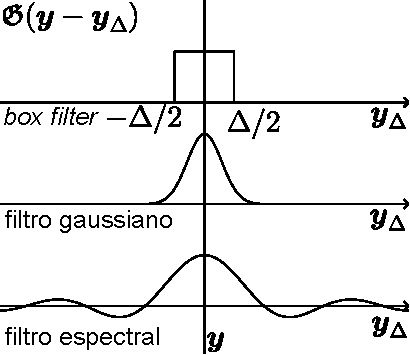
\includegraphics[width=\linewidth]{Figuras/filtros1.pdf}
        \caption{Função filtro.}
    \end{subfigure}
    \begin{subfigure}{0.4\textwidth}
        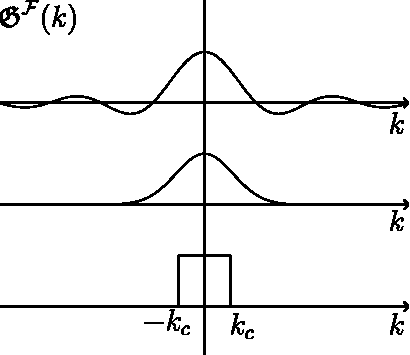
\includegraphics[width=\linewidth]{Figuras/filtros2.pdf}
        \caption{Transformada de Fourier.}
    \end{subfigure}
    \\Fonte: Autoria Própria (\the\year).
    \label{fig:Filters}
\end{figure}

O valor $\gamma_g$ observado no filtro gaussiano é uma constante, comumente atribuída com o valor de 6,0. Já o parâmetro $k_c$ é o número de onda de corte, dado por $k_c=\pi/\Delta$. Dentre os filtros apresentados, percebe-se que tanto o \textit{box filter} quanto o filtro gaussiano possuem suporte compacto no espaço físico, porém não possuem suporte compacto no espaço de Fourier, o que pode gerar problemas numéricos. Já o filtro espectral possui suporte compacto no espaço de Fourier, porém não possui suporte compacto no espaço físico.

Dessa maneira, é possível separar os efeitos das grandes escalas e das pequenas escalas, o que é ilustrado na Figura \ref{fig:EfeitoFiltragem} para uma distribuição de velocidade $\BB{u}$.

\begin{figure}[h!]
    \centering
    \caption{Efeito da filtragem sobre um campo de velocidades $\BB{u}$.}
    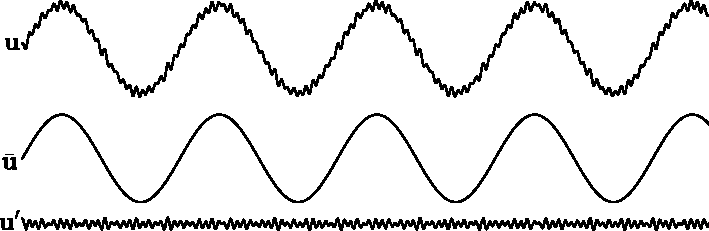
\includegraphics[width=.75\linewidth]{Figuras/efeito_filtragem.pdf}
    \\Fonte: \citeonline{hughes2000large} - Adaptado.
    \label{fig:EfeitoFiltragem}
\end{figure}

Assim, em uma descrição Euleriana, pode-se obter as equações de Navier-Stokes filtradas:

\begin{subequations}
    \begin{align}
         & \rho\bigpar{\dot{\BBB{u}}+\Ny\cdot(\overline{\BB{u}\otimes\BB{u}})-\BBB{f}}-\Ny\cdot\bar{\tens}=\BB{0} &  & \text{ em }\Omega\text{,} \\
         & \Ny\cdot\BBB{u}=0                                                                                      &  & \text{ em }\Omega\text{.}
    \end{align}
\end{subequations}

Pode-se perceber que o termo convectivo impede a completa separação dos termos $\BBB{u}$ e $\BB{u}'$ devido à sua natureza altamente não-linear. Por conta disso a parcela não filtrada não pode ser ignorada nesse problema, sendo necessário realizar algumas manipulações algébricas. Sabendo-se que $\BB{u}=\BBB{u}+\BB{u}'$, pode-se reescrever a equação da conservação da quantidade de movimento como:

\begin{equation}
    \rho\bigpar{\dot{\BBB{u}}+\Ny\cdot(\overline{(\BBB{u}+\BB{u}')\otimes(\BBB{u}+\BB{u}')})-\BBB{f}}-\Ny\cdot\bar{\tens}=\BB{0}
\end{equation}

Nesse sentido, surgirão termos cruzados entre $\BBB{u}$ e $\BB{u}'$, os quais serão condensados em um tensor de subescala (\textit{Subgrid-Scale} - SGS) $\BB{T}$ dado por \cite{piomelli1999large,hughes2000large}:

\begin{equation}
    \BB{T}=\BBB{u}\otimes\BBB{u}-\overline{\BB{u}\otimes\BB{u}}=-\bigpar{\BB{L}+\BB{C}+\BB{R}}\text{,}
\end{equation}

\noindent no qual $\BB{L}=\overline{\BBB{u}\otimes\BBB{u}}-\BBB{u}\otimes\BBB{u}$ é o tensor de Leonard, que representa as interações entre as grandes escalas, podendo ser determinado explicitamente e utilizado para análise de erros, $\BB{C}=\overline{\BBB{u}\otimes\BB{u}'}+\overline{\BB{u}'\otimes\BBB{u}}$ é o tensor de termos cruzados, representando a interação entre as grandes e pequenas escalas e $\BB{R}=\overline{\BB{u}'\otimes\BB{u}'}$ é o tensor de tensões SGS de Reynolds, que representa a interação entre as pequenas escalas \cite{piomelli1999large}. Assim pode-se escrever:

\begin{equation}
    \rho\bigpar{\dot{\BBB{u}}+\Ny\cdot(\BBB{u}\otimes\BBB{u})-\Ny\cdot\BB{T}-\BBB{f}}-\Ny\cdot\bar{\tens}=\BB{0}\text{.}
\end{equation}

Aplicando a incompressibilidade e substituindo-se $\bar{\tens}$ pelo modelo constitutivo \eqref{eq:ModConst}, tem-se que:

\begin{equation}
    \rho\bigpar{\dot{\BBB{u}}+(\BBB{u}\cdot\Ny)\BBB{u}-\Ny\cdot\BB{T}-\BBB{f}}-\mu\Ny\cdot(\Ny\BBB{u}+\NyT\BBB{u})+\Ny p=\BB{0}\text{,}\label{eq:ConMasLES}
\end{equation}

\noindent ou, dividindo-se por $\rho$ e fazendo algumas manipulações tem-se que:

\begin{equation}
    \dot{\BBB{u}}+(\BBB{u}\cdot\Ny)\BBB{u}+\frac{\Ny p}{\rho}=\nu\Lapl\BBB{u}+\Ny\BB{T}+\BBB{f}\text{,}
\end{equation}

\noindent sendo $\Lapl(\cdot)=\Ny\cdot\Ny(\cdot)$ o operador laplaciano e $\nu=\mu/\rho$ a viscosidade cinemática.

Assim, o problema fica governado por:

\begin{equation}
    \left\{
    \begin{array}{ll}
        \dot{\BBB{u}}+(\BBB{u}\cdot\Ny)\BBB{u}+\frac{\Ny p}{\rho}=\nu\Lapl\BBB{u}+\Ny\cdot\BB{T}+\BBB{f} & \text{ em }\Omega\text{,} \\
        \Ny\cdot\BBB{u}=0                                                                                & \text{ em }\Omega\text{,}
    \end{array}
    \right.
\end{equation}

\noindent havendo ainda a necessidade de se determinar um tensor $\BB{T}$, em especial o seu tensor desviador:

\begin{equation}
    \dev{\BB{T}}=\BB{T}-\frac{1}{3}\tr{(\BB{T})}\BB{I}\text{,}
\end{equation}

\noindent que descreva adequadamente as interações entre diferentes escalas. Isso pode se tornar problemático uma vez que não se possui solução para as pequenas escalas. Uma forma de se fazer isso é através do modelo de viscosidade de vórtice de Smagorinsky \cite{smagorinsky1963general}, resultando no tensor:

\begin{equation}
    \bigpar{\BB{T}_S}=2\nu_T\deffil\text{,}
\end{equation}

\noindent sendo $\nu_T$ a viscosidade de vórtice SGS, dada por \cite{germano1991dynamic,piomelli1999large,hughes2000large,bailly2015turbulence,katopodes2019free}:

\begin{equation}
    \nu_T=(C_S\Delta)^2\norm{\deffil}\text{,}
\end{equation}

\noindent onde $C_S$ é a constante de Smagorinsky e $\norm{\deffil}$ é a magnitude do tensor taxa de deformação em escala grosseira, dada por:

\begin{equation}
    \norm{\deffil}=(2\deffil:\deffil)^{1/2}\text{.}
\end{equation}

Note que o tensor $\BB{T}_S$ é um tensor desviador, ou seja, $\BB{T}_S=\dev{\BB{T}_S}$.

%\citeonline{germano1991dynamic,hughes2000large} ainda fazem algumas constatações sobre o modelo de Smagorinsky, os quais destacam-se o fato de $\BB{T}_S$ não possuir um comportamento assintótico próximo às paredes, o que se esperaria de $\BB{T}$, os valores de $C_S$ na presença de cisalhamento médio causaram amortecimentos excessivos e o tensor $\BB{T}_S$ impede a energia de fluir entre diferentes escalas, podendo ser significante em alguns casos.
%
%Como tentativa de se resolver esses problemas, \citeonline{germano1991dynamic} propuseram assumir $C_S$ como uma função $C_S=C_S(\BB{y},t)$, permitindo, assim, que esse parâmetro se adapte para melhor modelar as pequenas escalas.

Para a determinação da constante de Smagorinsky, realiza-se inicialmente uma aproximação da amplitude espectral da energia cinética $E(k)$, dada sobre a superfície de uma esfera parametrizada de raio $k$, de acordo com \cite{hughes2000large}:

\begin{equation}
    E(k)\approx\alpha\varepsilon^{2/3}k^{-5/3}\text{,}\label{eq:Ek1}
\end{equation}

\noindent em que $\alpha$ é a constante de Kolmogoroff e $\varepsilon$ é a dissipação turbulenta. A Figura \ref{fig:EnergiaEspectral} apresenta graficamente o comportamento da energia espectral em função de $k$.

\begin{figure}[h!]
    \centering
    \caption{Amplitude da energia espectral.}
    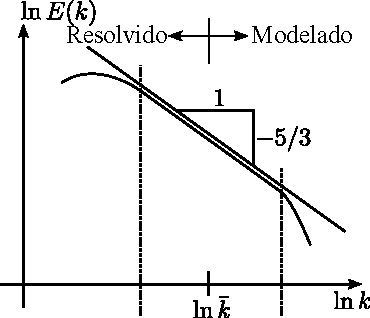
\includegraphics[width=0.4\linewidth]{Figuras/EnergiaEspectral.pdf}
    \\Fonte: \cite{hughes2000large} - Adaptado.
    \label{fig:EnergiaEspectral}
\end{figure}

O valor de $\norm{\deffil}$ é adotado como:

\begin{equation}
    \frac{1}{2}\norm{\deffil}=\int_0^{k_c}{k^2E(k)dk}\text{,}\label{eq:ndeffil1}
\end{equation}

\noindent sendo $k_c$ o limite de resolução.

Substituindo \eqref{eq:Ek1} em \eqref{eq:ndeffil1}, resolvendo a integral e fazendo algumas manipulações algébricas, tem-se que:

\begin{equation}
    \norm{\deffil}^3=\bigpar{\frac{3\alpha}{2}}^{3/2}k_c^2\varepsilon\text{.}
\end{equation}

Com isso, considerando também que a dissipação de energia cinética é igual àquela produzida, realiza-se o balanço da energia, obtendo-se:

\begin{equation}
    \varepsilon=\BB{T}_S:\deffil\text{.}
\end{equation}

\noindent Assim, fica possível obter expressões que relacionam os valores de $C_S$ $\Delta$ e $\nu_T$ com $k_c$:

\begin{equation}
    C_S\Delta=\bigpar{\frac{2}{3\alpha}}^{3/4}k_c^{-1}\text{ e}
\end{equation}

\begin{equation}
    \nu_T=\bigpar{\frac{2}{3\alpha}}\varepsilon^{1/3}k_c^{-4/3}\text{.}
\end{equation}

Segundo \citeonline{bailly2015turbulence} o valor de $k_c$ pode ser estimado como $k_c=\pi/\Delta$, o que leva à seguinte expressão para a constante de Smagorinsky:

\begin{equation}
    C_S=\frac{1}{\pi}\bigpar{\frac{2}{3\alpha}}^{3/4}\text{.}
\end{equation}

Com isso, um possível valor para a constante Kolmogoroff é $\alpha=1,4$, o que resulta em $C_S\approx0,18$. No entanto, segundo  \citeonline{hughes2000large,bailly2015turbulence,katopodes2019free}, valores de $C_S$ próximos à 0,10 conduzem a solução à resultados mais realistas.

\begin{comment}
%==================================================================================================
\subsubsection{Procedimento computacional} \label{LES-PC}
%==================================================================================================

Para a obtenção dos resultados, parte-se para a formulação variacional, em que se utiliza funções testes $\BB{w}$ e $q$, associadas às equações de conservação da quantidade de movimento e da continuidade, respectivamente. Assim, a forma fraca do problema LES é dada por:

\begin{equation}
    \begin{split}
        &\intDom{w_i\rho\bigpar{\dot{\ub}_i+\uub{j}\ub_{i,j}-\bar{f}_i}}+\intDom{\rho w_{i,j}T_{ij}}+\intDom{w_{i,j}\sigma_{ji}(\BB{\ub},\pb)}+\\
        &\intDom{q\ub_{i,i}}-\intNeumann{\rho w_iT_{ij}n_j}-\intNeumann{w_i\bar{h}_i}=0\text{.}
    \end{split}
\end{equation}

Substituindo o modelo constitutivo e o modelo de viscosidade de Smagorinsky tem-se que:

\begin{equation}
    \begin{split}
        &\intDom{w_i\rho\bigpar{\dot{\ub}_i+\uub{j}\ub_{i,j}-\bar{f}_i}}+\intDom{w_{i,j}(\mu+\rho\nu_T)(\uSim{\ub}{i}{j})}-\\
        &\intDom{w_{i,i}\pb}+\intDom{q\ub_{i,i}}-\intNeumann{w_i\bar{h}_i}=0\text{.}
    \end{split}
\end{equation}

\textcolor{purple}{
    No intuito de se obter uma solução estável, será considerado o elemento de Taylor-Hood P2P1 (aproximação quadrática para o campo de velocidades e linear para o campo de pressões) na formulação. Assim denomina-se $M$ as funções de forma para aproximação quadrática e $N$ para funções de forma lineares. Com isso, faz-se a aproximação das funções testes por meio das funções de forma, tendo como resultado os seguintes vetores de resíduo associados às equações de conservação de momento e da continuidade:
}
\textcolor{red}{1. Você deve deixar a formulação geral, e nos exemplos dizer o que você utilizou para obter resposta estável. Sugiro que desde o início (VMS) você diferencie as funções de forma de pressão e de velocidade (eu prefiro colocar um sobrescrito u e p ao invés de usar N e M). Aqui você deveria apresentar a formulação estabilizada, e nos exemplos você diz o que adotou para rodar. De qualquer forma, aqui ficou faltando colocar a estabilização para a convecção (SUPG) que sempre será necessária. Reveja o restante deste item com base nisso...}

\begin{subequations}
    \begin{equation}
        \begin{split}
            \bigpar{N_M}_i^a=&\intDom{M_a\rho\bigpar{\dot{\ub}_i+\uub{j}\ub_{i,j}-\bar{f}_i}}+\\
            &\intDom{M_{a,j}(\mu+\rho\nu_T)(\uSim{\ub}{i}{j})}-\intDom{M_{a,i}\pb}-\intNeumann{N_a\bar{h}_i}\text{ e}
        \end{split}
    \end{equation}
    \begin{equation}
        \bigpar{N_C}^a=\intDom{N_a\ub_{i,i}}\text{.}
    \end{equation}
    \label{eq:VetoresResiduo-LES}
\end{subequations}

Dessa forma procura-se determinar valores de $\ub$ e $\pb$ que anulem $N_M$ e $N_C$. Para esse fim utiliza-se o método de Newton-Raphson, em que as variáveis a serem determinadas são as acelerações e pressões nodais, sendo o integrador utilizado o $\alpha$-generalizado, apresentado na seção \ref{IT-VMS}. Desse modo tem-se os seguintes sub-blocos que compõem a matriz tangente:

\begin{subequations}
    \begin{equation}
        \begin{split}
            \der{(N_M)_i^a}{\dot{U}_j^b}=&\alpha_m\intDom{\rho M_aM_b}\dij+\beta_f\intDom{\rho M_aM_b\ub_{i,j}}+\\
            &\beta_f\intDom{\rho M_aM_{b,k}\uub{k}}\dij+\beta_f\intDom{(\mu+\rho\nu_T)M_{a,k}M_{d,k}}\dij+\\
            &\beta_f\intDom{(\mu+\rho\nu_T)M_{a,j}M_{b,i}}\text{,}
        \end{split}
    \end{equation}
    \begin{equation}
        \der{(N_M)_i^a}{P^b}=-\intDom{M_{a,i}N_b}\text{,}
    \end{equation}
    \begin{equation}
        \der{(N_C)^a}{\dot{U}_j^b}=\beta_f\intDom{N_aM_{b,j}}\text{ e}
    \end{equation}
    \begin{equation}
        \der{(N_C)^a}{P^b}=0\text{.}
    \end{equation}
    \label{eq:MatrizTangente-LES}
\end{subequations}

\noindent em que $\beta_f=\alpha_f\gamma\Delta t$.

Observa-se que o sub-bloco $\partial{\NC}/\partial\BB{P}$ está presente na diagonal principal do problema, possuindo valor nulo. Isso pode ser interpretado como a consideração das pressões como multiplicadores de Lagrange nessa formulação.

%Para obtenção da solução aproximada, utiliza-se um procedimento similar ao apresentado no algoritmo \ref{alg:MEF-VMS}, onde o comando \ref{alg:estabilizador} é alterado para computar o valor da viscosidade de vórtice, assim como os valores das componentes da matriz tangente e dos vetores de resíduo são alterados para se adequarem ao presente modelo.
\end{comment}
%==================================================================================================
\subsection{\textit{Reynolds-Averaged Navier-Stokes}} \label{RANS}
%==================================================================================================

A aproximação das equações diferenciais denominada \textit{Reynolds-Averaged Navier-Stokes} (RANS) busca encontrar uma solução a partir da chamada decomposição de Reynolds. Nesse contexto, observa-se que simulações feitas utilizando RANS são mais eficientes computacionalmente que aquelas feitas a partir de LES, além de possuírem uma implementação mais simples \cite{alfonsi2009reynolds, ling2015evaluation}.

Considera-se que uma propriedade $\phi$ pode ser decomposta em duas parcelas: uma referente à média, denotada por uma barra ($\bar{\phi}(\BB{y},t)$), e uma referente à flutuações no espaço-tempo, denotada por $\phi'(\BB{y},t)$, ou seja, $\phi(\BB{y},t)=\bar{\phi}+\phi'$.

No entanto, há diferentes formas de se considerar a média de uma propriedade, tal como: média temporal, comumente utilizada em escoamentos estacionários; média espacial, utilizada em escoamentos turbulentos homogêneos; e média de um conjunto de experimentos \cite{tennekes1972first,speziale1991analytical,alfonsi2009reynolds}. Como apontado por \citeonline{speziale1991analytical,alfonsi2009reynolds}, a última opção é adequada para descrever escoamentos que não são nem estacionários, nem homogêneos, sendo calculada como:

\begin{equation}
    \bar{\phi}(\BB{y},t)=\lim_{n\to\infty}{\frac{1}{n}\sum_{k=1}^n{\phi^{k}(\BB{y},t)}}\text{,}
\end{equation}

\noindent em que $n$ é o número de experimentos realizados.

Vale ressaltar algumas propriedades interessantes relacionadas à média de uma propriedade ($\phi$, $\phi_1$ ou $\phi_2$ quaisquer), tais como:

\begin{enumerate}[label=\alph*.]
    \item $\bar{\phi}'=0$;
    \item $\bar{\bar{\phi}}=\bar{\phi}$;
    \item $\bar{\phi_1+\phi_2}=\bar{\phi}_1+\bar{\phi}_2$;
    \item $\bar{\phi_1\bar{\phi}_2}=\bar{\phi}_1\bar{\phi}_2$;
    \item $\bar{\phi_1\phi_2}=\bar{\phi}_1\bar{\phi}_2+\bar{\phi_1'\phi_2'}$;
    \item $\bar{\Ny\phi}=\Ny\bar{\phi}$; e
    \item $\bar{\dot{\phi}}=\dot{\bar{\phi}}$.
\end{enumerate}

Assim, pode-se tomar a média das Equações de Navier-Stokes, obtendo-se:

\begin{subequations}
    \begin{align}
         & \rho\bigpar{\bar{\dot{\BB{u}}}+\bar{\Ny\cdot(\BB{u}\otimes\BB{u})}-\BBB{f}}-\bar{\Ny\cdot\tens}=\BB{0} &  & \text{ em }\Omega\text{,} \\
         & \bar{\Ny\cdot\BB{u}}=0                                                                                 &  & \text{ em }\Omega\text{.}
    \end{align}
\end{subequations}

Aplicando também o modelo constitutivo apresentado em \ref{MC}, o problema se torna:

\begin{subequations}
    \begin{align}
         & \rho\bigpar{\dot{\BBB{u}}+\Ny\cdot(\bar{\BB{u}\otimes\BB{u}})-\BBB{f}}-\mu\Lapl\BBB{u}+\Ny\bar{p}=\BB{0} &  & \text{ em }\Omega\text{,} \\
         & \Ny\cdot\BBB{u}=0                                                                                        &  & \text{ em }\Omega\text{.}
    \end{align}
\end{subequations}

Realizando a separação das variáveis em suas respectivas parcelas na equação da conservação de movimento, tem-se que:

\begin{equation}
    \rho\bigpar{\dot{\BBB{u}}+\Ny\cdot\bar{(\BBB{u}+\BB{u}')\otimes(\BBB{u}+\BB{u}')}-\BBB{f}}-\mu\Lapl{\BBB{u}}+\Ny\bar{p}=\BB{0}\text{,}
\end{equation}

\noindent que leva à seguinte expressão simplificada:

\begin{equation}
    \rho\bigpar{\dot{\BBB{u}}+\BBB{u}\cdot\Ny\BBB{u}+\Ny\cdot(\bar{\BB{u}'\otimes\BB{u}'})-\BBB{f}}-\mu\Lapl\BBB{u}+\Ny\bar{p}=\BB{0}\text{,}
    \label{eq:RANS-estac}
\end{equation}

\noindent a qual representa a equação RANS da quantidade de movimento para escoamentos incompressíveis \cite{chou1945velocity,alfonsi2009reynolds}.

Nesse contexto vale mencionar o tensor de tensões de Reynolds (dividido pela densidade), dado por $\btau=-\bar{\BB{u}'\otimes\BB{u}'}$, traz a interferência que os efeitos turbulentos que a parcela de flutuação causa no movimento médio \cite{chou1945velocity,alfonsi2009reynolds}. Porém, verifica-se que, ao assumir essa separação de variáveis, o problema conta com mais incógnitas do que equações para as determinar. Logo, uma forma de se obter equações adicionais que auxiliem na resolução do problema se encontra na modelagem do tensor de tensões de Reynolds de forma a relacionar as flutuações de velocidades com as velocidades médias.

\citeonline{alfonsi2009reynolds} aponta que problemas envolvendo RANS podem ser classificados dependendo da quantidade de equações diferenciais resolvidas, em que cada equação adicionada se refere ao transporte de uma propriedade relativa à turbulência, alterando, assim, a maneira com que a viscosidade de vórtice é determinada. Segundo o autor, as classes de modelos RANS de turbulência são:

\begin{enumerate}[label=\alph*.]
    \item Modelos de Zero Equações: Apenas as equações referentes ao campo médio são resolvidas, sendo $l_0$ e $\tau_0$ determinados empiricamente;
    \item Modelos de Uma Equação: É adicionada uma equação de transporte em termos da energia cinética média $k$ para auxiliar na determinação do campo de flutuações de velocidades;
    \item Modelos de Duas Equações: Uma segunda equação é adicionada para determinação das escalas de comprimento turbulento;
    \item Modelos de Tensões: A respeito aos Modelos de Zero Equações, adiciona-se duas equações de transporte referentes ao tensor de Reynolds e à $\varepsilon$, tal modelo também pode ser chamado de modelo $\te$.
\end{enumerate}

Sobre os Modelos de Duas Equações, destacam-se os modelos $\ke$ \cite{haakansson2012experimental,davidson2014pans,parente2011improved}, nos quais as equações adicionais são dadas em função da energia cinética média gerada pelo campo de flutuações ($k$) e da taxa de dissipação da energia cinética turbulenta ($\varepsilon$) e $\kw$ \cite{larsen2018over,bassi2005discontinuous}, que ao invés de adicionar uma equação em termos de $\varepsilon$, esta de dá em função da escala de tempo turbulento recíproco ($\omega=\varepsilon/K$).

Dentre os modelos $\ke$, $\kw$ e $\te$, observa-se que o primeiro possui menor custo computacional e maior facilidade de implementação, sendo uma boa alternativa para as simulações \cite{koutsourakis2012evaluation,adanta2020comparison}.

Para se obter as equações adicionais, faz-se a simples substituição de $\BB{u}=\umed+\BB{u}'$ e $p=\bar{p}+p'$ na equação da quantidade de movimento, o que leva a:

\begin{equation}
    \begin{split}
        &\rho\bigpar{\dot{\BBB{u}}+\dot{\BB{u}'}+\BBB{u}\cdot\Ny\BBB{u}+\BBB{u}\cdot\Ny\BB{u}'+\BB{u}'\cdot\Ny\BBB{u}+\BB{u}'\cdot\Ny\BB{u}'-\BBB{f}}-\mu\Lapl\BBB{u}-\\
        &\mu\Lapl\BB{u}'+\Ny\bar{p}+\Ny p'=\BB{0}\text{.}
    \end{split}
    \label{eq:NS-RANS1}
\end{equation}

Subtraindo \eqref{eq:RANS-estac} de \eqref{eq:NS-RANS1} obtém-se:

\begin{equation}
    \rho\bigpar{\dot{\BB{u}'}+\BBB{u}\cdot\Ny\BB{u}'+\BB{u}'\cdot\Ny\BBB{u}+\BB{u}'\cdot\Ny\BB{u}'-\Ny\cdot\btau}-\mu\Lapl\BB{u}'+\Ny p'=\BB{0}\text{.}
    \label{eq:NS-RANS2}
\end{equation}

Seguindo o mesmo procedimento para a equação da conservação da massa obtém-se que:

\begin{equation}
    \Ny\cdot\BB{u}'=0\text{,}
\end{equation}

\noindent sendo equivalente à condição de incompressibilidade no campo de flutuações de velocidade.

Fazendo a contração em \eqref{eq:NS-RANS2} por meio de $\BB{u}'$, tomando a média, dividindo por $\rho$ e realizando as devidas simplificações tem-se a equação que descreve de forma exata o comportamento da energia cinética média gerada pelo campo de flutuações ($K=\bar{\norm{\BB{u}'}^2}/2$) \cite{alfonsi2009reynolds}:

%\begin{equation}
%    \bar{\BB{u}'\cdot\dvt{\BB{u}'}}+\bar{\BB{u}'\cdot(\BBB{u}\cdot\Ny\BB{u}')}+\bar{\BB{u}'\cdot(\BB{u}'\cdot\Ny\BBB{u})}+\bar{\BB{u}'\cdot(\BB{u}'\cdot\Ny\BB{u}')}+\bar{\BB{u}'\cdot(\Ny\cdot\btau)}-\bar{\nu\BB{u}'_i\cdot\Lapl\BB{u}'}+\bar{\BB{u}'\cdot\Ny\pr'}=0\text{.}
%\end{equation}

\begin{equation}
    \dot{K}+\BBB{u}\cdot\Ny K=\btau:\Ny\BBB{u}-\frac{\nu}{2}\bar{\norm{\Ny\BB{u}'}^2}-\Ny\cdot\bigpar{\frac{\bar{\norm{\BB{u}'}^2\BB{u}'}}{2}+\bar{\pr'\BB{u}'}}+\nu\Lapl K\text{,}
    \label{eq:Ke-K}
\end{equation}

\noindent em que $\pr'=p'/\rho$. Assim, \eqref{eq:Ke-K} pode ainda ser reescrita de forma mais compacta, considerando-se o efeito de cada parcela:

\begin{equation}
    \dot{K}+\BBB{u}\cdot\Ny K=P_K-\varepsilon-\Ny\cdot\BB{D}+\nu\Lapl K\text{,}
\end{equation}

\noindent em que $P_K$ é a produção da energia cinética turbulenta, a qual não precisa de modelagem, $\varepsilon$ é a taxa de dissipação turbulenta da energia cinética, $D_j$ é o gradiente de difusão turbulenta e o último termo, que dispensa modelagem, representa a difusão viscosa. Tais termos são dados por:

\begin{subequations}
    \begin{align}
         & P_K=\btau:\Ny\BBB{u}\text{,}                                             \\
         & \varepsilon=\frac{\nu}{2}\bar{\norm{\Ny\BB{u}'}^2}\text{ e}              \\
         & \BB{D}=\frac{\bar{\norm{\BB{u}'}^2\BB{u}'}}{2}+\bar{\pr'\BB{u}'}\text{.}
    \end{align}
\end{subequations}

\citeonline{alfonsi2009reynolds} apresenta que uma forma de se modelar os termos $\varepsilon$ e $\BB{D}$ como:

\begin{subequations}
    \begin{equation}
        \varepsilon=C^*\frac{K^{3/2}}{l_0}\text{ e}\\
    \end{equation}
    \begin{equation}
        \BB{D}=-\frac{\nu_T}{\sigma_K}\Ny K\text{,}
    \end{equation}
\end{subequations}

\noindent sendo $l_0$ o comprimento de vórtice, $C^*=0,166$ e $\sigma_K=1,0$ constantes adimensionais.

Há ainda a necessidade de se modelar o tensor de Reynolds, o qual pode ser subdividido em duas parcelas: uma parte isotrópica ($\btau^\mathrm{I}$) e outra desviadora ($\btau^\mathrm{D}$), ou seja:

\begin{equation}
    \btau=\btau^\mathrm{I}+\btau^\mathrm{D}\text{,}
\end{equation}

\noindent em que:

\begin{subequations}
    \begin{align}
         & \btau^\mathrm{I}=-\frac{2}{3}K\BB{I}\text{ e} \\
         & \btau^\mathrm{D}=2\nu_T\epmean\text{,}
    \end{align}
\end{subequations}

\noindent $\epmean_{ij}$ é a taxa de deformação do campo de velocidades média:

\begin{equation}
    \epmean=\frac{1}{2}(\Ny\BBB{u}+\NyT\BBB{u})
\end{equation}

\noindent e $\nu_T$ é a viscosidade de vórtice, dada por

\begin{equation}
    \nu_T=C_\mu\frac{K^2}{\varepsilon}\text{,}
\end{equation}

\noindent sendo $C_\mu=0,09$.

Já a equação exata do transporte que descreve a taxa de dissipação turbulenta da energia cinética ($\ep$) também é proveniente da equação \eqref{eq:NS-RANS2}, onde toma-se o gradiente da equação, realiza-se a contração dupla por meio de $\nu\Ny\BB{u}'/\rho$ e toma-se a média de todos os termos. Assim, após as simplificações tem-se, em sua forma indicial:

\begin{equation}
    \begin{split}
        &\dot{\ep}+\bar{u}_k\ep_{,k}=-2\nu\bar{u'_{i,j}u'_{k,j}}\bar{u}_{i,k}-2\nu\bar{u'_{i,j}u'_{i,k}}\bar{u}_{k,j}-2\nu\bar{u'_{i,j}u'_k}\bar{u}_{i,jk}-\\
        &2\nu\bar{u'_{i,j}u'_{k,j}u'_{i,k}}-\nu\bigpar{\bar{u'_{i,j}u'_{i,j}u'_k}}_{,k}-2\nu(\bar{u'_{i,j}\pr'_{,j}})_{,i}-2\nu^2\bar{u'_{i,jk}u'_{i,jk}}+\nu\ep_{,kk}\text{,}
    \end{split}
\end{equation}

\noindent sendo a vírgula presente no subíndice referente à derivada na direção indicada.

Fazendo a simplificação em termos dos efeitos de cada parcela tem-se:

\begin{equation}
    \dot{\ep}+\uub{k}\ep_{,k}=P_\ep+D_\ep-\Phi_\ep+\nu\ep_{,kk}\text{,}
\end{equation}

\noindent em que $P_\ep$ é a produção de dissipação, $D_\ep$ é a difusão turbulenta de dissipação, $\Phi_\ep$ é a destruição turbulenta da dissipação e o último termo é o transporte viscoso. Essas parcelas são dadas de forma exata por:

\begin{subequations}
    \begin{align}
         & P_\ep=-2\nu\bar{u'_{i,j}u'_{k,j}}\bar{u}_{i,k}-2\nu\bar{u'_{i,j}u'_{i,k}}\bar{u}_{k,j}-2\nu\bar{u'_{i,j}u'_k}\bar{u}_{i,jk}-2\nu\bar{u'_{i,j}u'_{k,j}u'_{i,k}} \text{,} \\
         & D_\ep=-\nu\bigpar{\bar{u'_{i,j}u'_{i,j}u'_k}}_{,k}-2\nu(\bar{u'_{i,j}\pr'_{,j}})_{,i} \text{ e}                                                                         \\
         & \Phi_\ep=2\nu^2\bar{u'_{i,jk}u'_{i,jk}}\text{.}
    \end{align}
\end{subequations}

Assim, realiza-se uma modelagem sobre os termos necessários como:

\begin{subequations}
    \begin{align}
         & P_\ep=C_{\ep 1}\frac{\ep}{k}\btau:\Ny\BBB{u}\text{,}          \\
         & D_\ep=\Ny\cdot\bigpar{\frac{\nu_T}{\sigma_\ep}\Ny\ep}\text{e} \\
         & \Phi_\ep=C_{\ep 2}\frac{\ep^2}{K}\text{,}
    \end{align}
\end{subequations}

\noindent em que $C_{\ep 1}=1,44$, $C_{\ep 2}=1,92$ e $\sigma_\ep=1,3$ são constantes adimensionais.

Assim, o problema RANS fica descrito pelas equações:

\begin{equation}
    \left\{
    \begin{array}{l}
        \rho\bigpar{\dot{\BBB{u}}+\BBB{u}\cdot\Ny\BBB{u}-\Ny\cdot\btau-\BBB{f}}-\mu\Lapl\BBB{u}+\Ny\bar{p}=\BB{0} \\
        \Ny\cdot\BBB{u}=0                                                                                         \\
        \dot{K}+\BBB{u}\cdot\Ny K=P_K-\varepsilon-\Ny\cdot\BB{D}+\nu\Lapl K                                       \\
        \dot{\varepsilon}+\BBB\cdot\Ny\ep=P_\ep+D_\ep-\Phi_\ep+\nu\Lapl\ep                                        \\
        \btau=-\frac{2}{3}K\BB{I}+\nu_T(\Ny\BBB{u}+\NyT\BBB{u})                                                   \\
        \nu_T=C_\mu\frac{K^2}{\ep}\text{.}
    \end{array}
    \right.
\end{equation}
%%==================================================================================================
\subsection{Exemplos Numéricos} \label{ExemplosMT}
%==================================================================================================

Na presente seção serão apresentadas algumas simulações realizadas utilizando os modelos VMS e LES, com a finalidade de validar os modelos implementados.

%==================================================================================================
\subsubsection{Cavidade bidimensional}
%==================================================================================================

A primeira simulação é um problema comumente utilizado na literatura como \textit{benchmark}, o qual trata-se de uma cavidade quadrada ($\Omega=[-1,1]^2$) com paredes aderentes, onde o fluido encontra-se confinado e sujeito a uma velocidade prescrita $\BB{u}_\infty$ ocasionada devido ao deslizamento de uma parede na face superior da cavidade. Nesse sentido serão observados os efeitos provocados no fluido devido à diferentes números de Reynolds, o qual é calculado por meio da equação \ref{eq:Reynolds}:

\begin{equation}
    \Rey=\frac{\rho L\norm{\BB{u}_\infty}}{\mu}\text{,}
    \label{eq:Reynolds}
\end{equation}

\noindent em que $L$ é o comprimento característico, que no caso analisado é igual ao lado da cavidade. Dessa forma considera-se uma velocidade constante para todas as análises de $\BB{u}_\infty=\{1,0\}^T$, sendo os diferentes números de Reynolds obtidos pela variação da viscosidade do fluido. A Figura \ref{fig:cavity} apresenta esquematicamente o problema simulado.

\begin{figure}[h!]
    \centering
    \caption{Desenho esquemático do problema de cavidade.}
    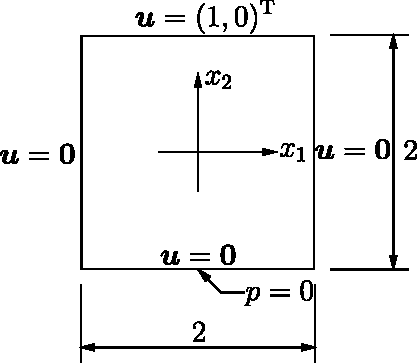
\includegraphics[width=.35\linewidth]{Figuras/Cavity/cavidade.pdf}
    \\Fonte: Autoria Própria (\the\year).
    \label{fig:cavity}
\end{figure}

Pelo fato do problema possuir apenas fronteiras do tipo Dirichlet, o condicionamento da solução do campo de pressões é garantido pela aplicação de uma condição de pressão nula no vértice superior direito da cavidade, conforme visto na figura acima.  Também se observa que existe uma descontinuidade nas condições de contorno no encontro entre as paredes da cavidade e seu topo, podendo ser consideradas velocidades nulas ou igual à velocidade do topo. No problema em questão considerou-se que a velocidade nesse ponto é igual à $\BB{u}_\infty$.

A malha de elementos finitos foi feita pela subdivisão do domínio em 20000 elementos dispostos de maneira estruturada com orientação à esquerda, conforme observado na Figura \ref{fig:cavity_disc}. O número de graus de liberdade para a simulação VMS de aproximação linear, quadrática e LES são 30603, 121203 e 91003, respectivamente. Os parâmetros utilizados foram $\rho=1$ para todas as análises, $\mu=0,02$, $\mu=5\times10^{-3}$, $\mu=2\times10^{-3}$, $\mu=4\times10^{-4}$, $\mu=2,6667\times10^{-4}$ e $\mu=2\times10^{-4}$, resultando em $\Rey=100$, $\Rey=400$, $\Rey=1000$, $\Rey=5000$, $\Rey=7500$ e $\Rey=10000$, respectivamente. Os modelos utilizados foram o VMS com aproximação linear e quadrática e o LES com elementos de Taylor-Hood P2P1 e $C_S=0,10$. O passo de tempo em todos os casos foi de $\Delta t=0,1$ e a simulação foi mantida até que a estacionariedade dos parâmetros do fluxo fosse alcançada.

\begin{figure}[h!]
    \centering
    \caption{Malha considerada para o problema de cavidade.}
    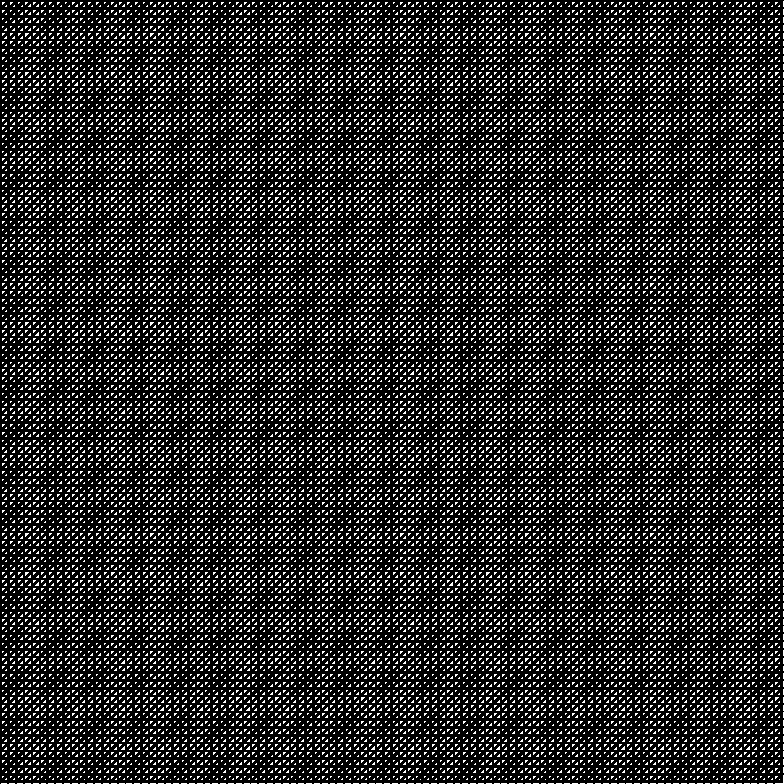
\includegraphics[width=.6\linewidth]{Figuras/Cavity/mesh.pdf}
    \\Fonte: Autoria Própria (\the\year).
    \label{fig:cavity_disc}
\end{figure}

Como o problema apresenta características de um escoamento quase-estático, a parcela dos termos inerciais foram desprezados em ambos os modelos de turbulência. Além disso, os resultados adquiridos para um determinado número de Reynolds foram aplicados como valores iniciais para a determinação dos resultados para a próxima análise.

Os resultados obtidos foram comparados com aqueles apresentados por \citeonline{ghia1982high}. A Figura \ref{fig:cavity-results} apresenta os valores do campo de velocidades sobre as linhas médias da cavidade ($x_1=0$ e $x_2=0$).

\begin{figure}[h!]
    \centering
    \caption{Valores do campo de velocidades sobre as linhas médias da cavidade.}
    \begin{subfigure}{0.4\textwidth}
        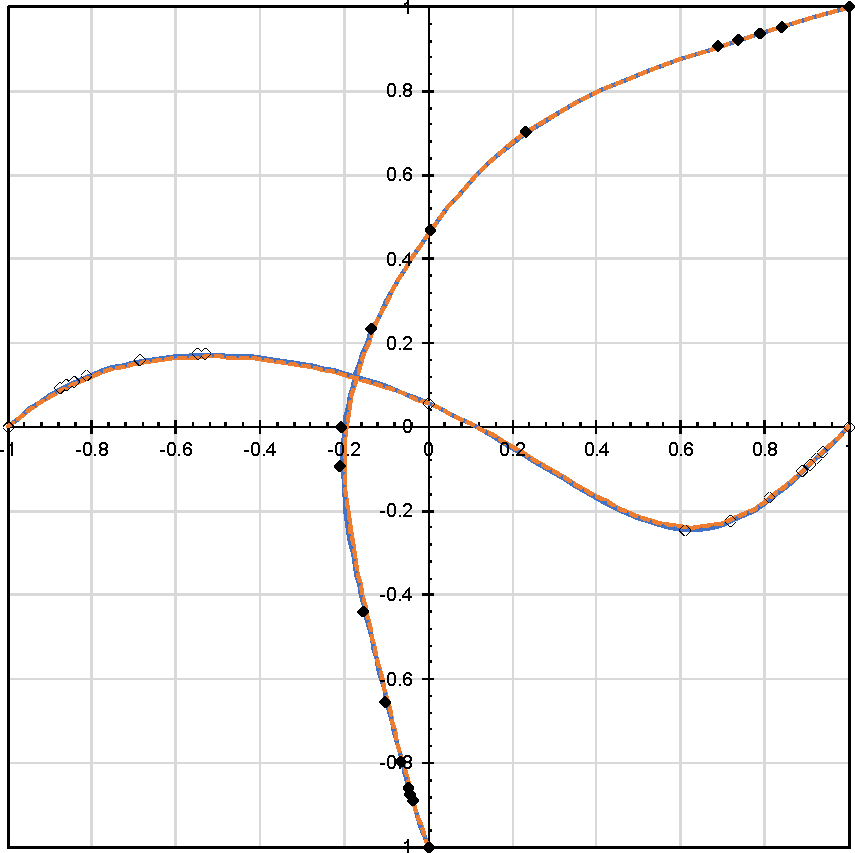
\includegraphics[width=\linewidth]{Figuras/Cavity/Re100.pdf}
        \caption{$\Rey=100$}
    \end{subfigure}
    \begin{subfigure}{0.4\textwidth}
        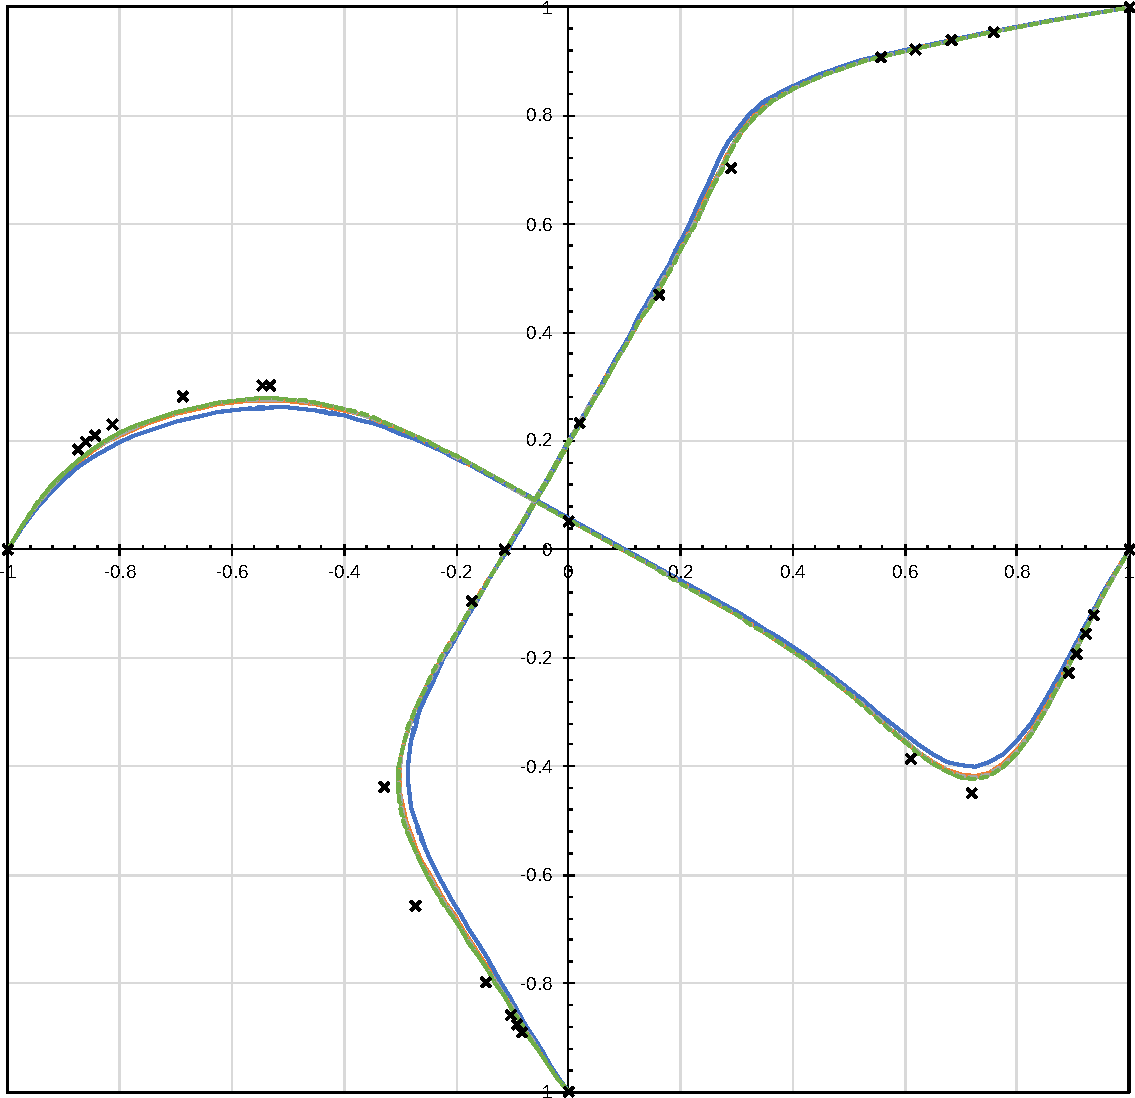
\includegraphics[width=\linewidth]{Figuras/Cavity/Re400.pdf}
        \caption{$\Rey=400$}
    \end{subfigure}
    \begin{subfigure}{0.4\textwidth}
        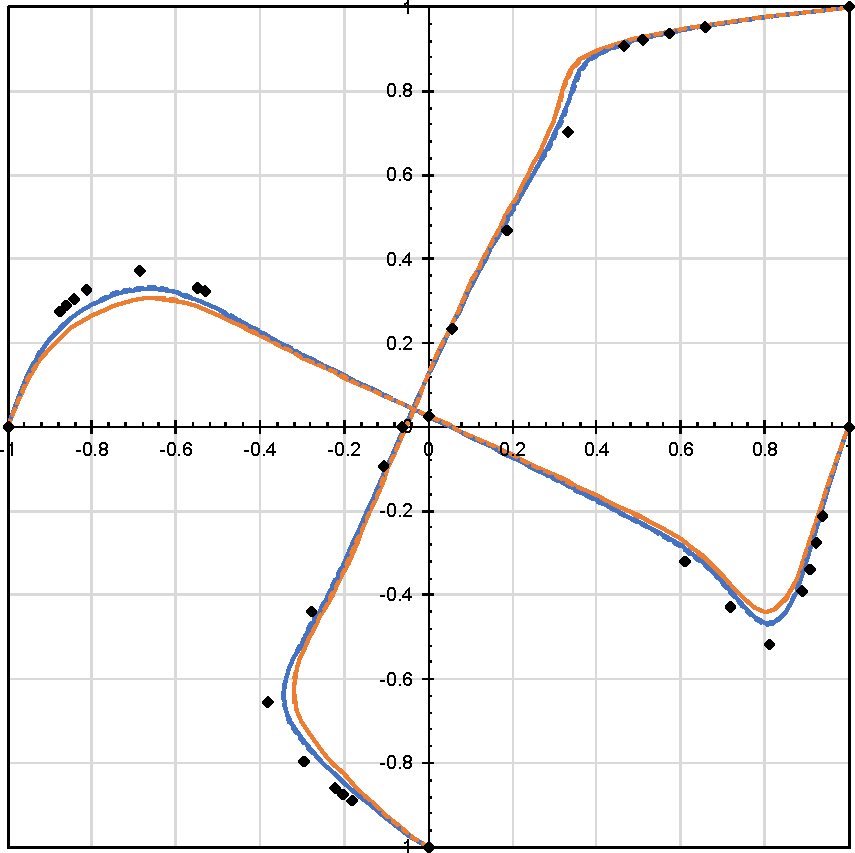
\includegraphics[width=\linewidth]{Figuras/Cavity/Re1000.pdf}
        \caption{$\Rey=1000$}
    \end{subfigure}
    \begin{subfigure}{0.4\textwidth}
        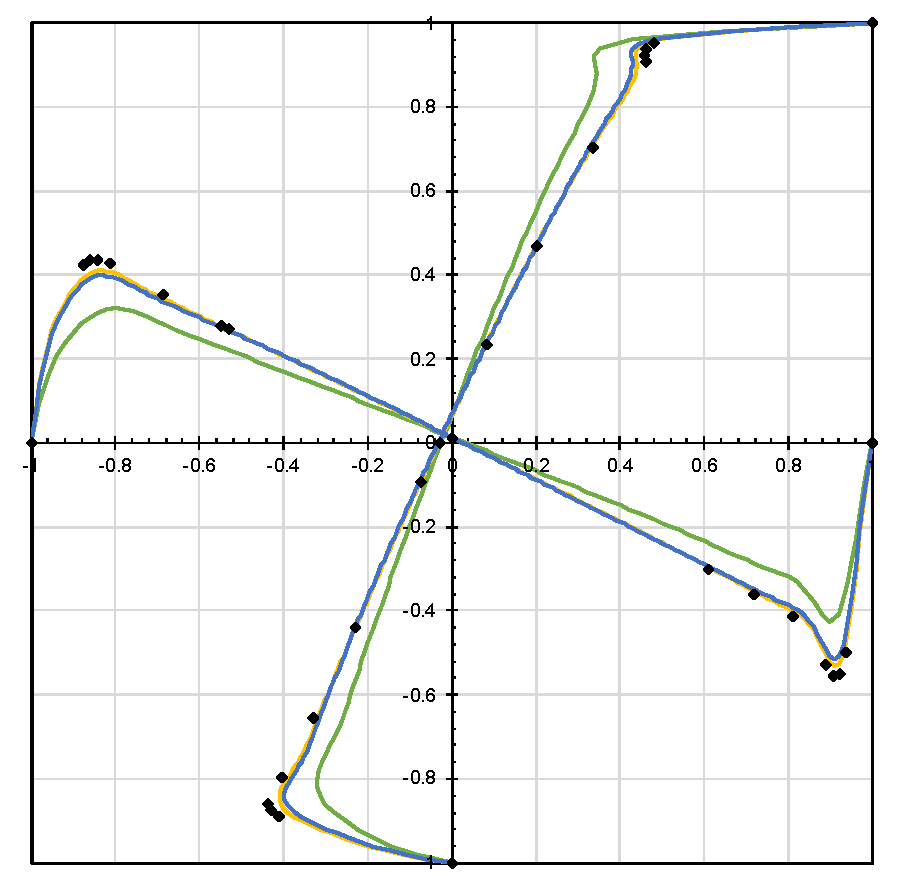
\includegraphics[width=\linewidth]{Figuras/Cavity/Re5000.pdf}
        \caption{$\Rey=5000$}
    \end{subfigure}
    \begin{subfigure}{0.4\textwidth}
        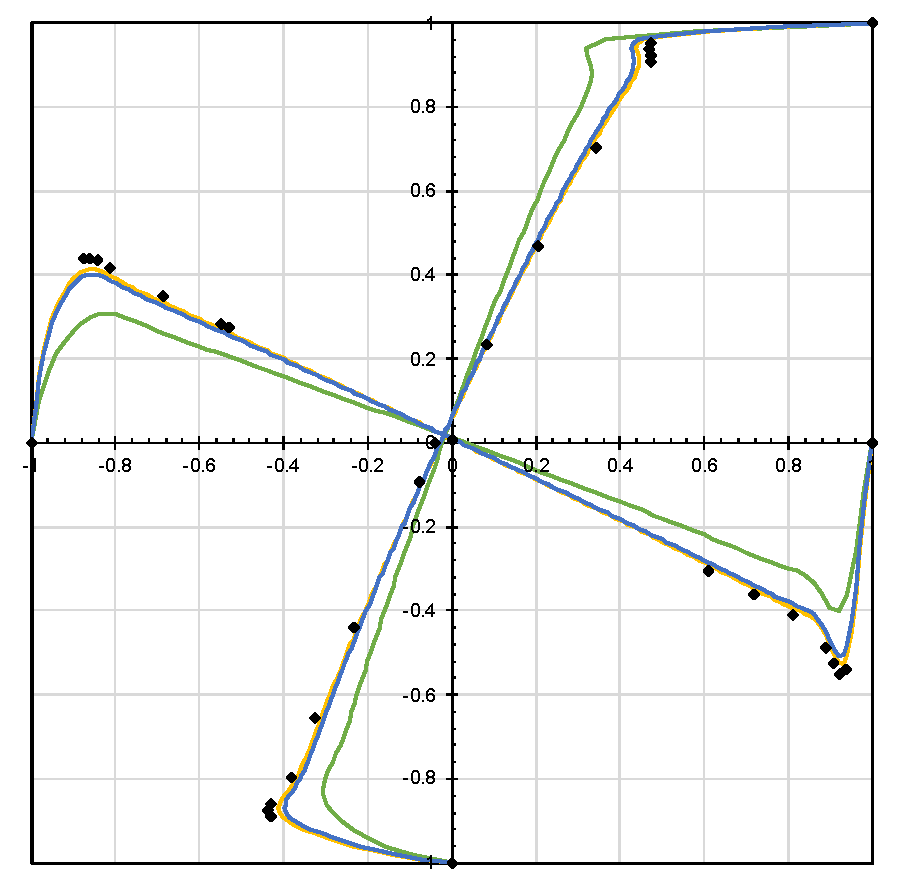
\includegraphics[width=\linewidth]{Figuras/Cavity/Re7500.pdf}
        \caption{$\Rey=7500$}
    \end{subfigure}
    \begin{subfigure}{0.4\textwidth}
        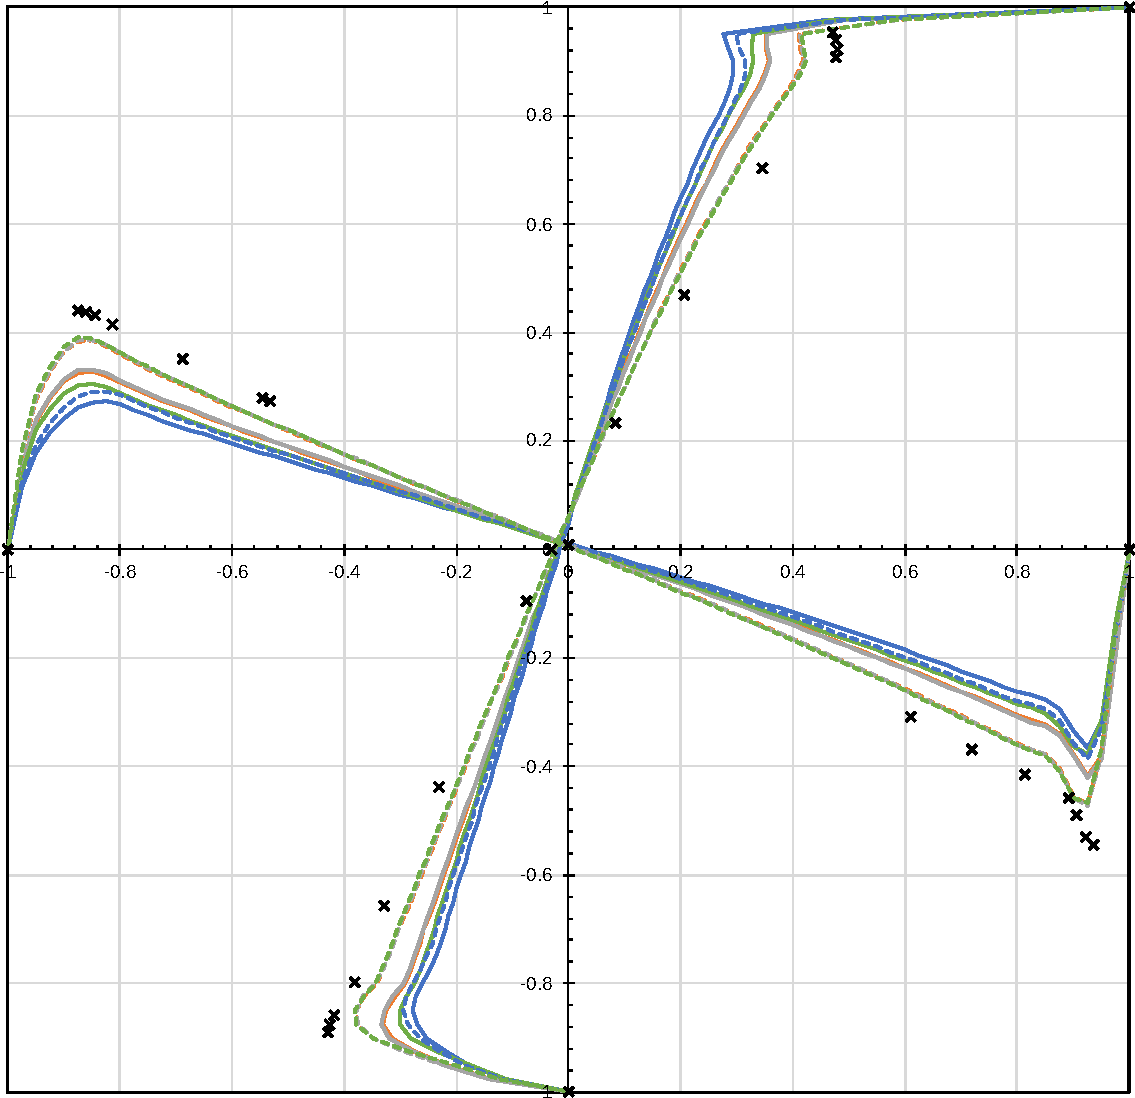
\includegraphics[width=\linewidth]{Figuras/Cavity/Re10000.pdf}
        \caption{$\Rey=10000$}
    \end{subfigure}
    \begin{subfigure}{\textwidth}
        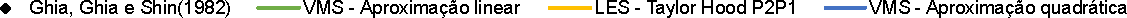
\includegraphics[width=\linewidth]{Figuras/Cavity/Legenda.pdf}
    \end{subfigure}
    \\Fonte: Autoria Própria (\the\year).
    \label{fig:cavity-results}
\end{figure}

A Figura \ref{fig:cavity-results2} apresenta o campo de velocidades na cavidade após o escoamento atingir seu estado estacionário.

\begin{figure}[h!]
    \centering
    \caption{Campo de velocidades em regime estacionário na cavidade.}
    \begin{subfigure}{0.32\textwidth}
        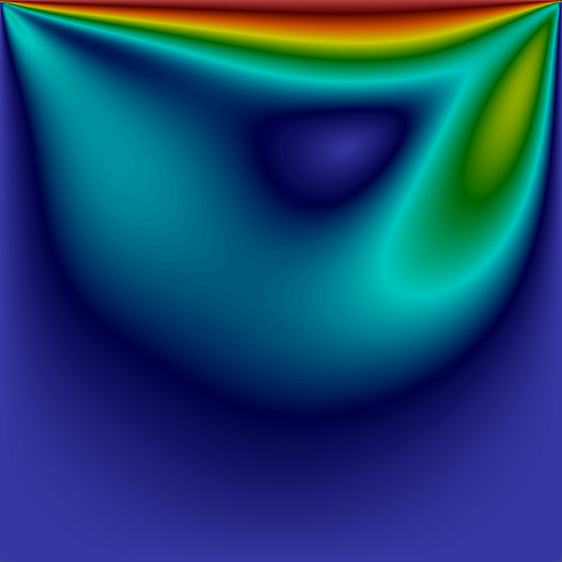
\includegraphics[width=\linewidth]{Figuras/Cavity/Re100.png}
        \caption{$\Rey=100$}
    \end{subfigure}
    \begin{subfigure}{0.32\textwidth}
        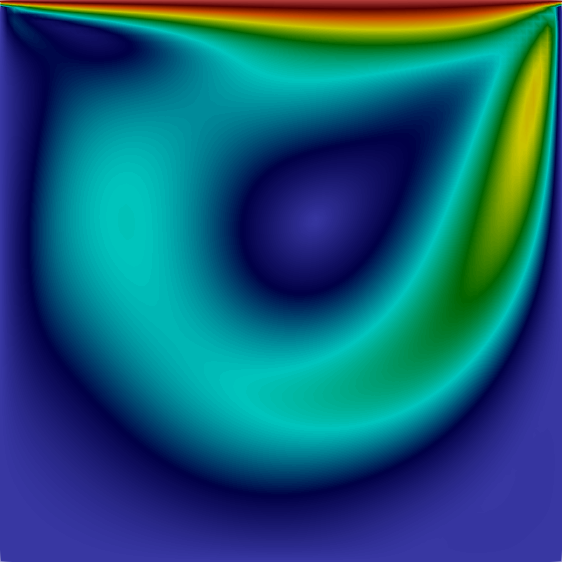
\includegraphics[width=\linewidth]{Figuras/Cavity/Re400.png}
        \caption{$\Rey=400$}
    \end{subfigure}
    \begin{subfigure}{0.32\textwidth}
        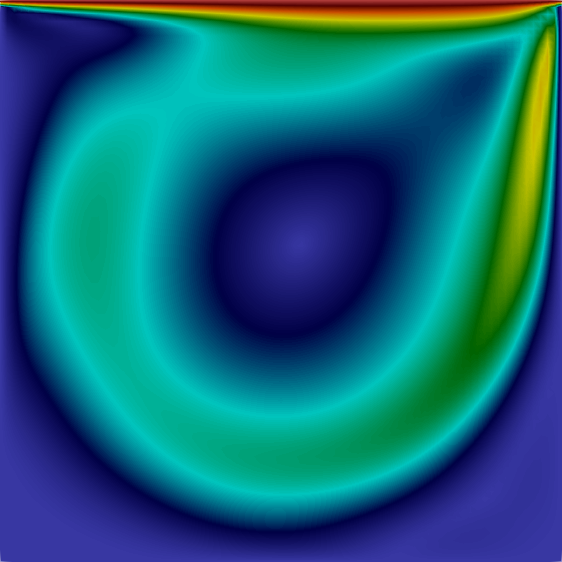
\includegraphics[width=\linewidth]{Figuras/Cavity/Re1000.png}
        \caption{$\Rey=1000$}
    \end{subfigure}
    \begin{subfigure}{0.32\textwidth}
        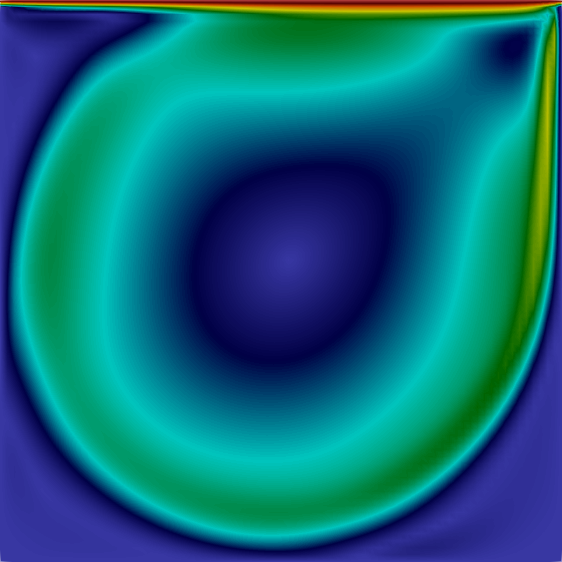
\includegraphics[width=\linewidth]{Figuras/Cavity/Re5000.png}
        \caption{$\Rey=5000$}
    \end{subfigure}
    \begin{subfigure}{0.32\textwidth}
        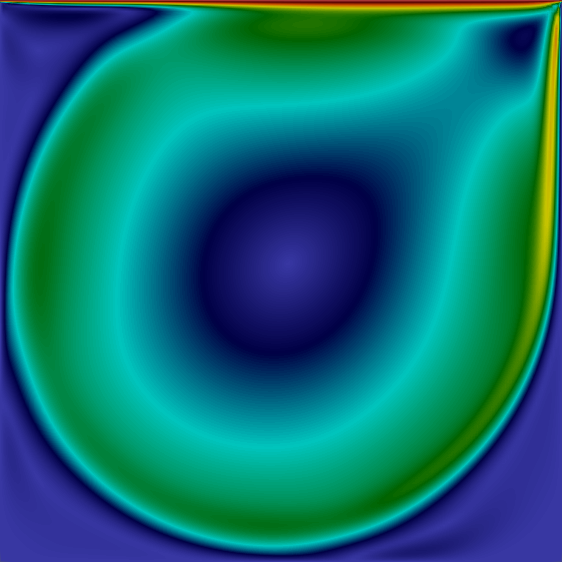
\includegraphics[width=\linewidth]{Figuras/Cavity/Re7500.png}
        \caption{$\Rey=7500$}
    \end{subfigure}
    \begin{subfigure}{0.32\textwidth}
        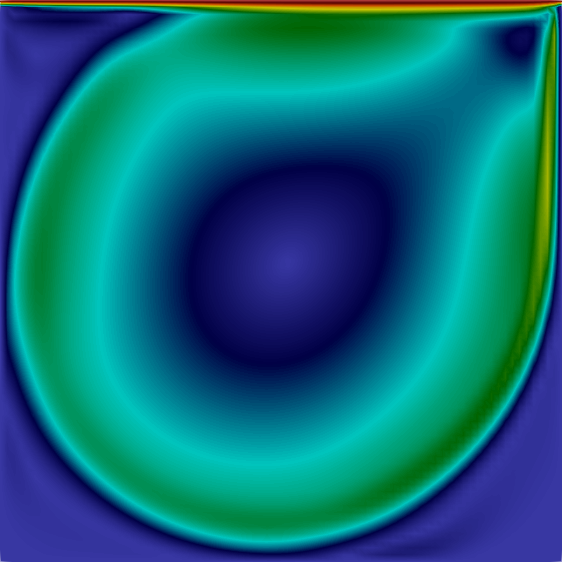
\includegraphics[width=\linewidth]{Figuras/Cavity/Re10000.png}
        \caption{$\Rey=10000$}
    \end{subfigure}
    \begin{subfigure}{0.4\textwidth}
        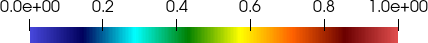
\includegraphics[width=\linewidth]{Figuras/Cavity/Legenda.png}
    \end{subfigure}
    \\Fonte: Autoria Própria (\the\year).
    \label{fig:cavity-results2}
\end{figure}

Para todas as simulações conduzidas, percebeu-se que houve uma excelente concordância dos resultados para números de Reynolds baixos, no entanto a simulação VMS de aproximação linear passou a apresentar resultados cada vez mais discrepantes à medida que o número de Reynolds aumentou, enquanto o VMS de aproximação quadrática e o LES apresentaram resultados mais próximos aos de \citeonline{ghia1982high}, sendo que o LES apresentou resultados ligeiramente melhores em relação ao VMS quadrático. Para número de Reynolds muito altos observou-se um leve desvio nos resultados próximos à parede superior da cavidade, o que poderia ser melhorado caso uma discretização mais fina da malha fosse empregada nessa região.

Para comparação da convergência entre os modelos implementados realizou-se um simulação com $\Rey=1000$ partindo de uma condição inicial $\BB{u}=\BB{0}$ em todo o domínio. As medidas de resíduos observadas foram relacionadas à velocidade ($e_u=\norm{\Delta\BB{U}}$) e à pressão ($e_p=\norm{\Delta\BB{P}}$) e a simulação foi conduzida até que um resíduo abaixo de $1\times10^{-8}$ fosse obtido. A Figura \ref{fig:comp-res} apresenta a convergência dos modelos segundo essas medidas.

\begin{figure}[h!]
    \centering
    \caption{Comparação do resíduo da:}
    \begin{subfigure}{\textwidth}
        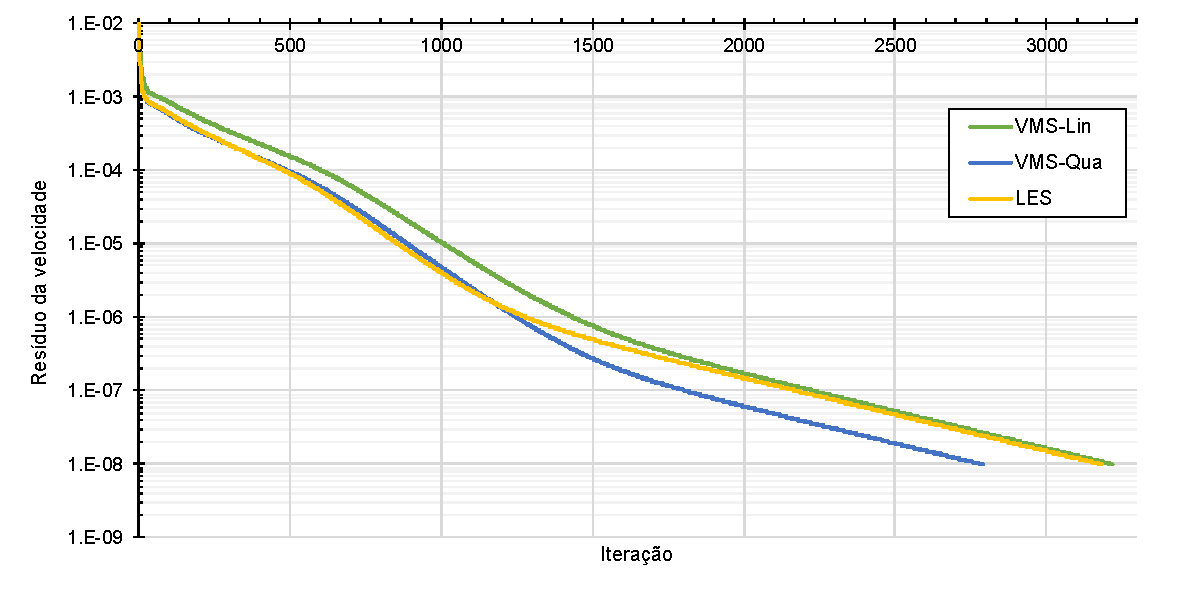
\includegraphics[width=\linewidth]{Figuras/Cavity/resvel.pdf}
        \caption{velocidade.}
    \end{subfigure}
    \begin{subfigure}{\textwidth}
        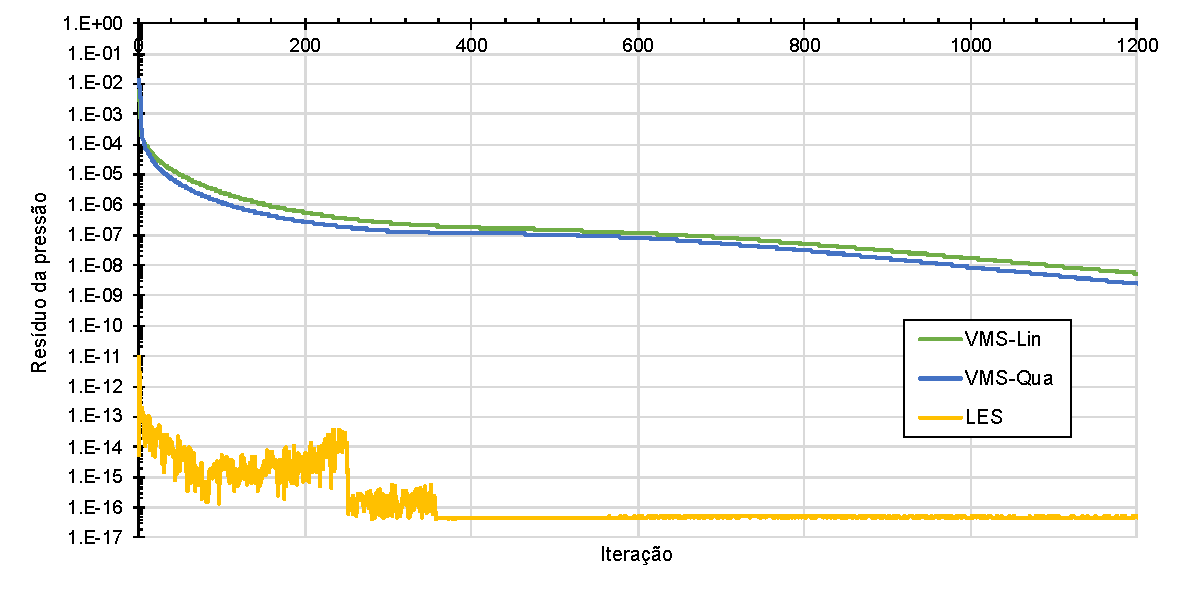
\includegraphics[width=\linewidth]{Figuras/Cavity/respre.pdf}
        \caption{pressão.}
    \end{subfigure}
    \\Fonte: Autoria Própria (\the\year).
    \label{fig:comp-res}
\end{figure}

Também foi observado o tempo necessário para que a convergência fosse atingida. A Tabela \ref{tab:comp-res} apresenta o número de iteração necessárias para que ambas as medidas de erro atingissem a tolerância, o tempo médio por iteração e o tempo total da simulação.

\begin{table}[h!]
    \centering
    \caption{Resultados do estudo de convergência dos métodos.}
    \begin{tabular}{lccc}
        \hline
        Modelo         & número de iterações & tempo por iteração (s) & tempo (min) \\\hline
        VMS linear     & 3218                & 0,650                  & 34,872      \\
        VMS quadrático & 2788                & 3,814                  & 177,260     \\
        LES            & 3182                & 3,494                  & 185,357     \\\hline
    \end{tabular}
    \\Fonte: Autoria Própria (\the\year).
    \label{tab:comp-res}
\end{table}

Observa-se no resíduo da velocidade que todos os métodos tiveram uma convergência mais rápida no início da simulação, pois um fluxo rotacional ainda estava sendo obtido pelos modelos. Após se estabelecer esse fluxo a convergência desacelerou até atingir a tolerância admitida. Já com relação ao resíduo da pressão verifica-se que o modelo LES obteve uma convergência imediata, no entanto a convergência dos demais modelos também foi rápida de tal forma a essa medida não ser o limitante em relação ao tempo de processamento. Ao final do processamento o VMS quadrático foi o que precisou da menor quantidade de iterações para convergir, no entanto, devido à quantidade de graus de liberdade ser maior, seu tempo requerido para cada iteração aumentou, necessitando de um tempo similar ao LES.

Por fim, verificou-se a necessidade da utilização do modelo de turbulência em simulações de malha menos refinada em situação de número de Reynolds elevado. Para isso assumiu-se um problema com $\Rey=10000$, sendo o domínio computacional gerado pela divisão de cada aresta em 20 segmentos, totalizando, assim, 800 elementos finitos triangulares, dispostos de forma estruturada com orientação à esquerda. As simulações foram conduzidas sem a utilização de nenhum modelo de turbulência, seguido dos modelos LES e VMS. Para cada uma das simulações empregou-se elementos de aproximação linear, quadrática e Taylor-Hood P2P1, sendo que para os dois primeiros aplicou-se um estabilizador PSPG, uma vez que esses elementos não possuem estabilidade no campo de pressões. Assim, chegou-se em 441 nós e 1323 DOF para a simulação contendo elementos lineares, 1681 nós e 5043 DOF para quadráticos e 1681 nós e 3803 DOF para P2P1. A simulação foi mantida em um intervalo de tempo $t\in[0,500]$, discretizado em $\Delta t=0,1$, sendo que a condição inicial foi de $\BB{u}=\BB{0}$ em todos os pontos no interior do domínio. A Tabela \ref{tab:comp-res2} apresenta de forma qualitativa os resultados obtidos. O campo de velocidades obtidos para cada simulação no instante $t=500$ é apresentado no Apêndice A.

\begin{table}[h!]
    \centering
    \caption{Comparação dos resultados apresentados em simulação em modelo, com aplicação de LES e de VMS.}
    \begin{tabularx}{\textwidth}{|p{2cm}|p{3cm}|X|}
        \hline
        Tipo de elemento      & Simulação  & Resultado                                                         \\\hline
        \MR{3}{*}{Linear}     & Sem modelo & Sem sentido físico                                                \\\cline{2-3}
                              & LES        & Formação de vórtice com valores espúrios próximos à face superior \\\cline{2-3}
                              & VMS        & Formação de vórtice com variação pequena do campo de velocidades  \\\hline
        \MR{3}{*}{Quadrático} & Sem modelo & Não houve avanço na solução (se manteve na condição inicial)      \\\cline{2-3}
                              & LES        & Formação de vórtice                                               \\\cline{2-3}
                              & VMS        & Formação de vórtice                                               \\\hline
        \MR{3}{*}{P2P1}       & Sem modelo & Divergência                                                       \\\cline{2-3}
                              & LES        & Não atingiu o regime permanente                                   \\\cline{2-3}
                              & VMS        & Formação de vórtice                                               \\\hline
    \end{tabularx}
    \\Fonte: Autoria Própria (\the\year).
    \label{tab:comp-res2}
\end{table}

Logo, verifica-se que as simulações sem a aplicação de modelos de turbulência não foi capaz de simular o comportamento do escoamento. Por outro lado, mesmo em uma situação de malha grosseira, as simulações empregando LES e VMS foram capazes de capturar esse comportamento. No entanto a simulação modelada por LES em elemento P2P1 não atingiu o regime permanente.

%==================================================================================================
\subsubsection{\textit{Taylor-Green Vortex} tridimensional}
%==================================================================================================

Para verificação dos modelos implementados em simulações tridimensionais é possível simular o problema de \textit{Taylor-Green Vortex} (TGV), o qual possui solução analítica, dada por \cite{shapiro1993use}:

\begin{subequations}
    \begin{equation}
        \begin{split}
            &\BB{u}_a(\BB{x},t)=\\
            &-\frac{Ae^{-\nu\lambda^2t}}{k^2+l^2}\begin{bmatrix}
                \lambda l\cos{(kx_1)}\sin{(lx_2)}\sin{(mx_3)}+mk\sin{(kx_1)}\cos{(lx_2)}\cos{(mx_3)} \\
                \lambda k\sin{(kx_1)}\cos{(lx_2)}\sin{(mx_3)}-ml\cos{(kx_1)}\sin{(lx_2)}\cos{(mx_3)} \\
                -(k^2+l^2)\cos{(kx_1)}\cos{(lx_2)}\sin{(mx_3)}
            \end{bmatrix}\text{,}
        \end{split}
    \end{equation}
    \begin{equation}
        p_a=p_s-\rho\frac{u_1^2+u_2+u_3^2}{2}\text{.}
    \end{equation}
\end{subequations}

\noindent em que $k$, $l$ e $m$ são constantes arbitrárias, $\lambda^2=k^2+l^2+m^2$, $A$ é a amplitude da componente $u_3$ e $p_s$ é a pressão do ponto de estagnação.

Para o problema numérico foi considerado um cubo ($\Omega=[-1,1]^3$) simulado nos modelos VMS de aproximação linear e quadrática e o LES utilizando elementos Taylor-Hood P2P1. A malha utilizada na discretização conta com 5802 elementos finitos (conforme ilustrado na Figura \ref{fig:TGV-mesh}), sendo 5580 graus de liberdade para VMS linear, 37600 pra VMS quadrático e 29595 para LES.

\begin{figure}[h!]
    \centering
    \caption{Malha utilizada para a simulação de TGV.}
    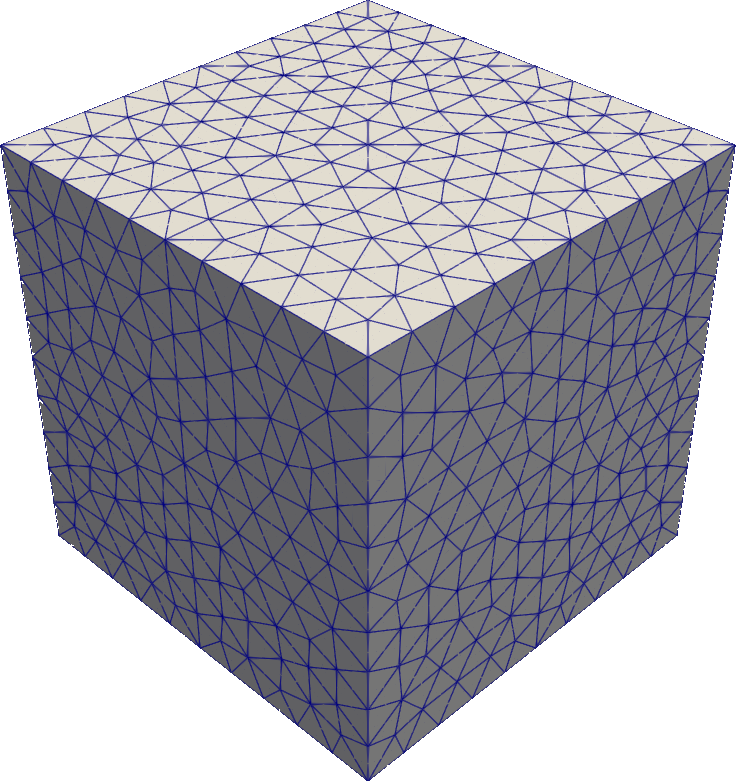
\includegraphics[width=0.4\linewidth]{Figuras/taylor-green/mesh.png}
    \\Fonte: Autoria Própria (\the\year).
    \label{fig:TGV-mesh}
\end{figure}

Como condição inicial impôs-se acelerações, velocidade e pressões iguais à solução analítica com $t=0$ e como condições de contorno aplicou-se velocidades iguais à analítica em toda a fronteira e $p=0$ no centro do domínio. Os valores dos parâmetros foram $k=l=m=\pi$ e $A=\nu=\rho=1$, sendo o período analisado de $t\in[0,0.2]$ com um passo de tempo de $\Delta t=0.001$.

Sendo assim, a Figura \ref{fig:TGV-results} apresenta os valores do campo de velocidades nas linhas $x_2=x_3=0$ ($l1$), $x_1=x_3=0$ ($l2$) e $x_1=x_2=0$ ($l3$) para os instantes $t=0$, $t=0.05$ e $t=0.2$ para todos os modelos considerados.

\begin{figure}[h!]
    \centering
    \caption{Velocidades obtidas na a simulação de TGV em:}
    \begin{subfigure}{0.42\textwidth}
        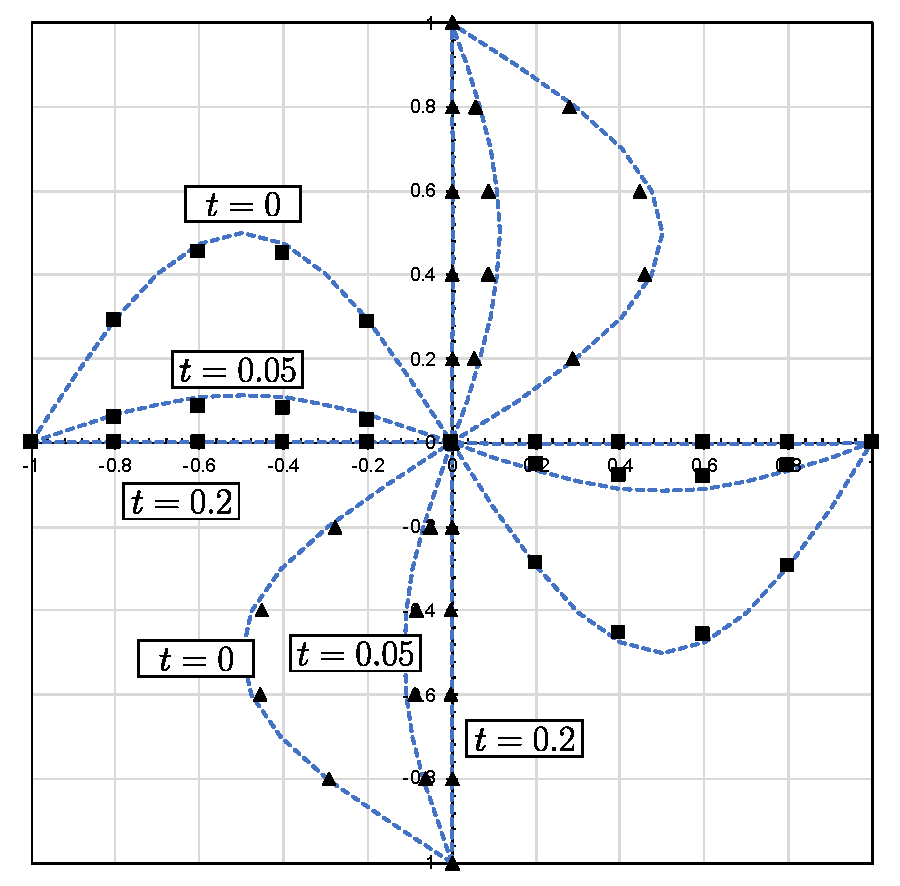
\includegraphics[width=\linewidth]{Figuras/taylor-green/VMS-Lin.pdf}
        \caption{$l1$ e $l2$ para VMS linear.}
    \end{subfigure}
    \begin{subfigure}{0.42\textwidth}
        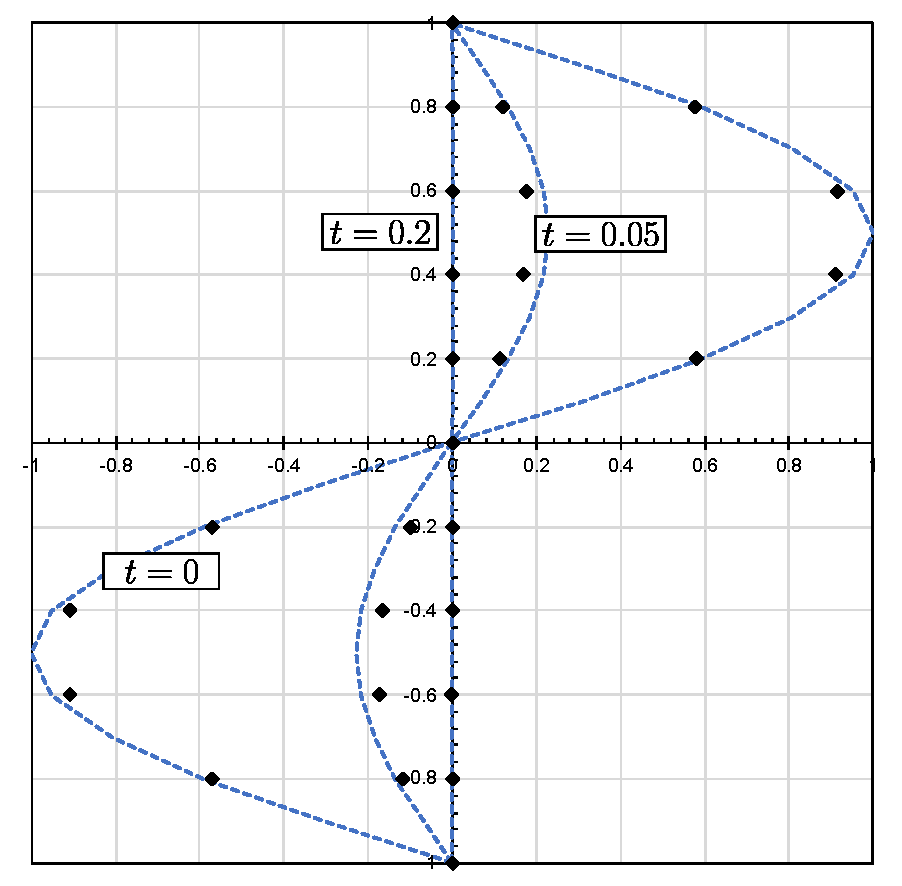
\includegraphics[width=\linewidth]{Figuras/taylor-green/VMS-Lin-uz.pdf}
        \caption{$l3$ para VMS linear.}
    \end{subfigure}
    \begin{subfigure}{0.42\textwidth}
        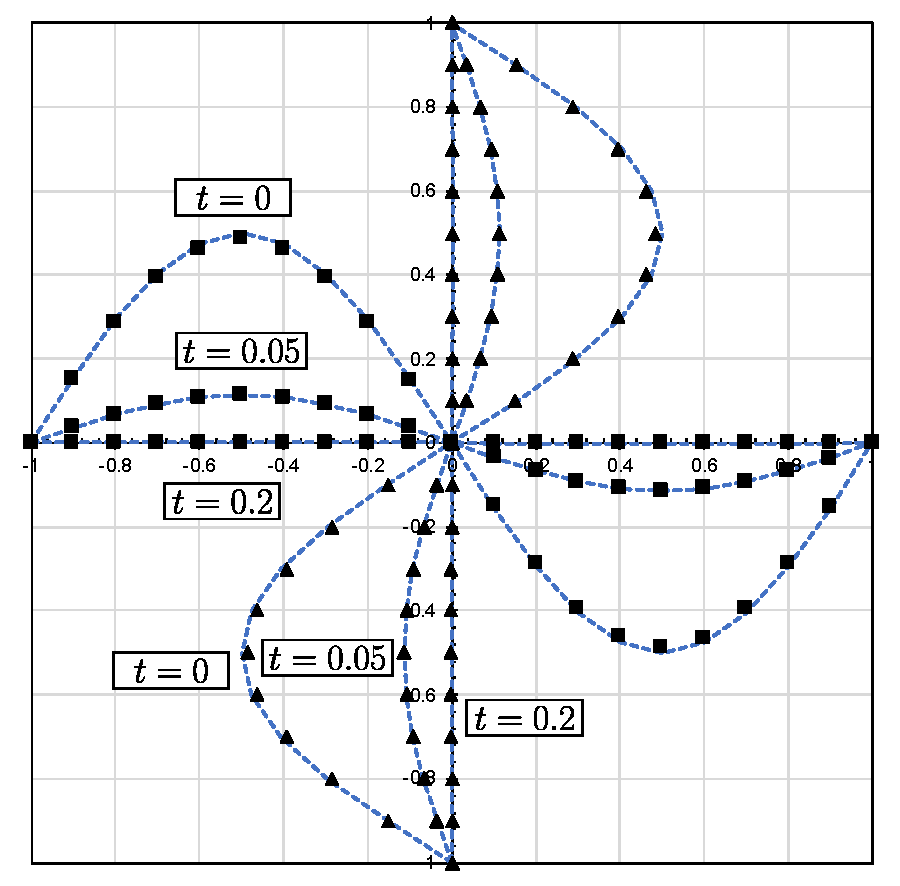
\includegraphics[width=\linewidth]{Figuras/taylor-green/VMS-Qua.pdf}
        \caption{$l1$ e $l2$ para VMS quadrático.}
    \end{subfigure}
    \begin{subfigure}{0.42\textwidth}
        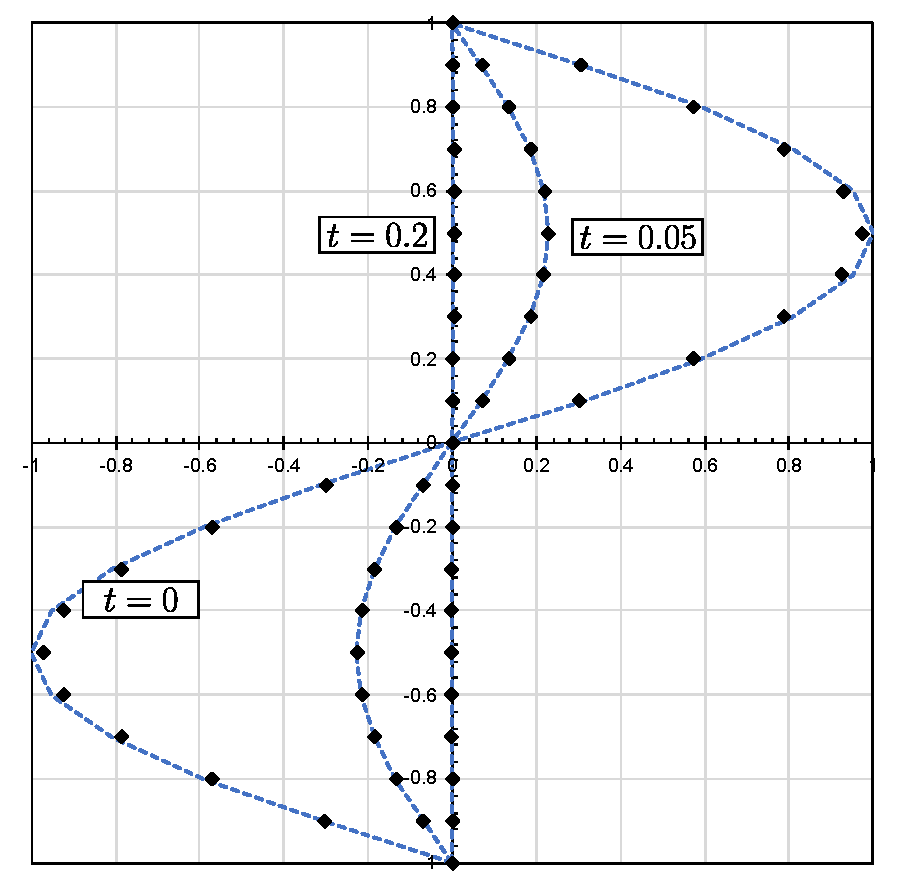
\includegraphics[width=\linewidth]{Figuras/taylor-green/VMS-Qua-uz.pdf}
        \caption{$l3$ para VMS quadrático.}
    \end{subfigure}
    \begin{subfigure}{0.42\textwidth}
        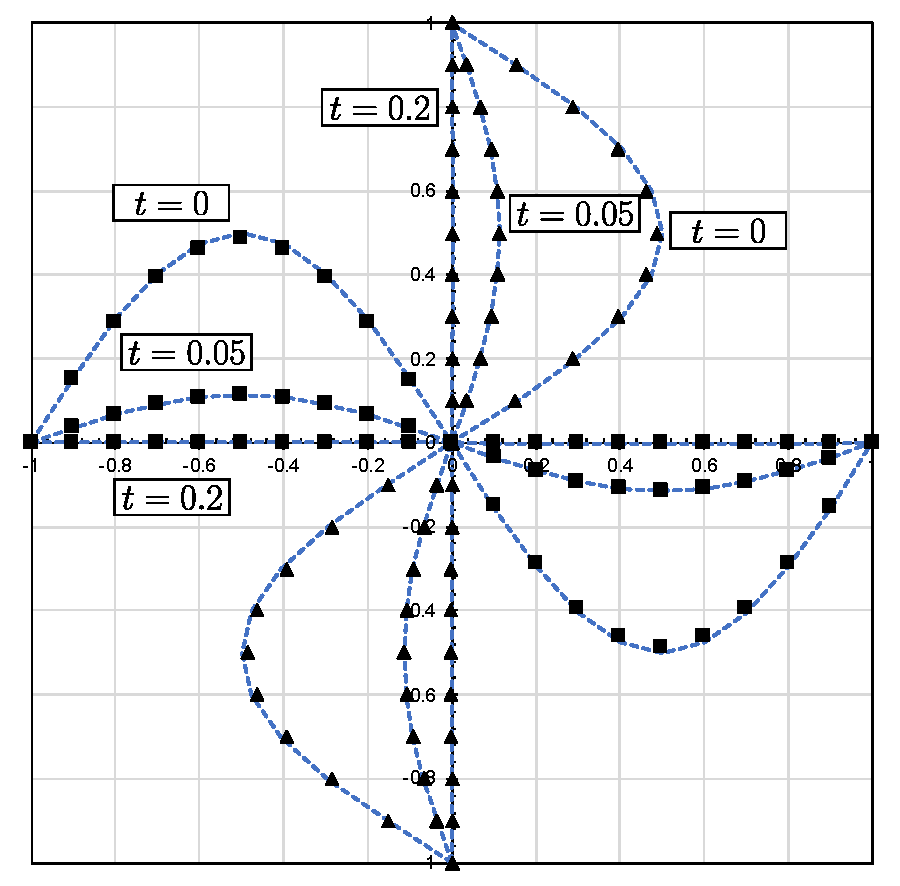
\includegraphics[width=\linewidth]{Figuras/taylor-green/LES.pdf}
        \caption{$l1$ e $l2$ para LES.}
    \end{subfigure}
    \begin{subfigure}{0.42\textwidth}
        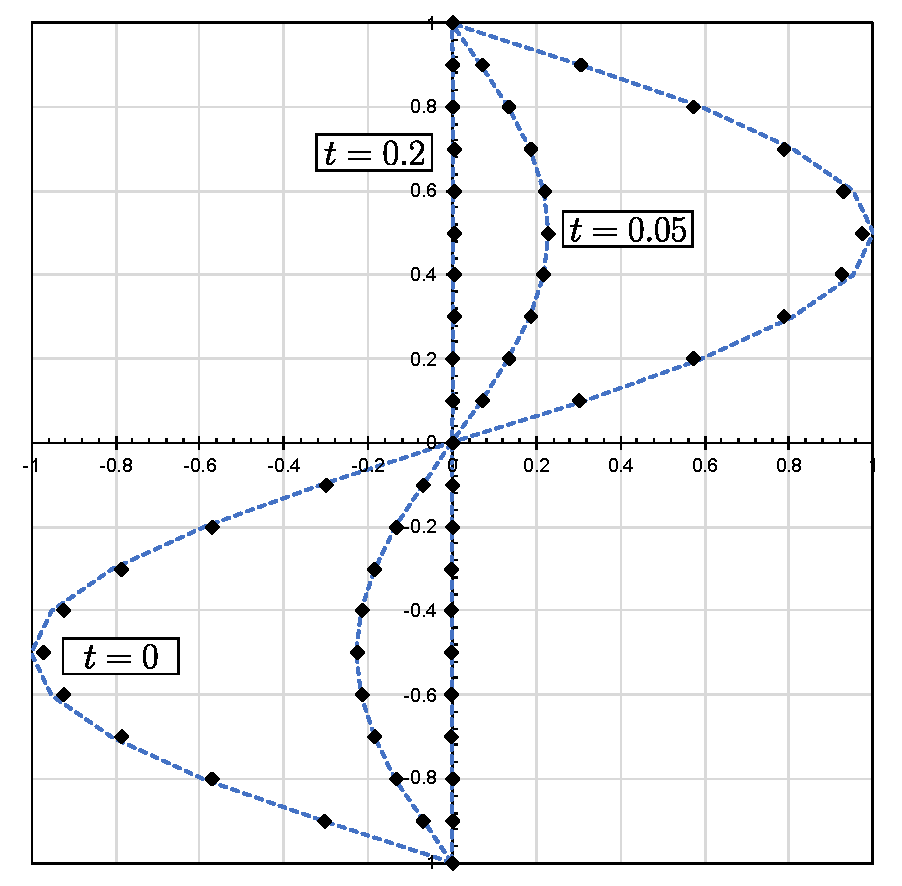
\includegraphics[width=\linewidth]{Figuras/taylor-green/LES-uz.pdf}
        \caption{$l3$ para LES.}
    \end{subfigure}
    \begin{subfigure}{0.42\textwidth}
        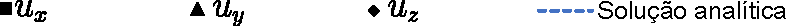
\includegraphics[width=\linewidth]{Figuras/taylor-green/legenda.pdf}
    \end{subfigure}
    \\Fonte: Autoria Própria (\the\year).
    \label{fig:TGV-results}
\end{figure}

Para comparação com a solução analítica, tomou-se a medida do erro em $L^2$, expresso por \cite{dumon2011proper}:

\begin{equation}
    \norm{\BB{e}}=\norm{\BB{u}-\BB{u}_a}_{L^\infty(L^2(\Omega))}=\max_{0<t\leq T}{\left[\int_\Omega{\norm{\BB{u}-\BB{u}_a}^2d\Omega}\right]}\text{,}
\end{equation}

\noindent o qual é representado ao longo do tempo de acordo com a Figura \ref{fig:TGV-L2}:

\begin{figure}[h!]
    \centering
    \caption{Medidas de $L^2$ ao longo do tempo.}
    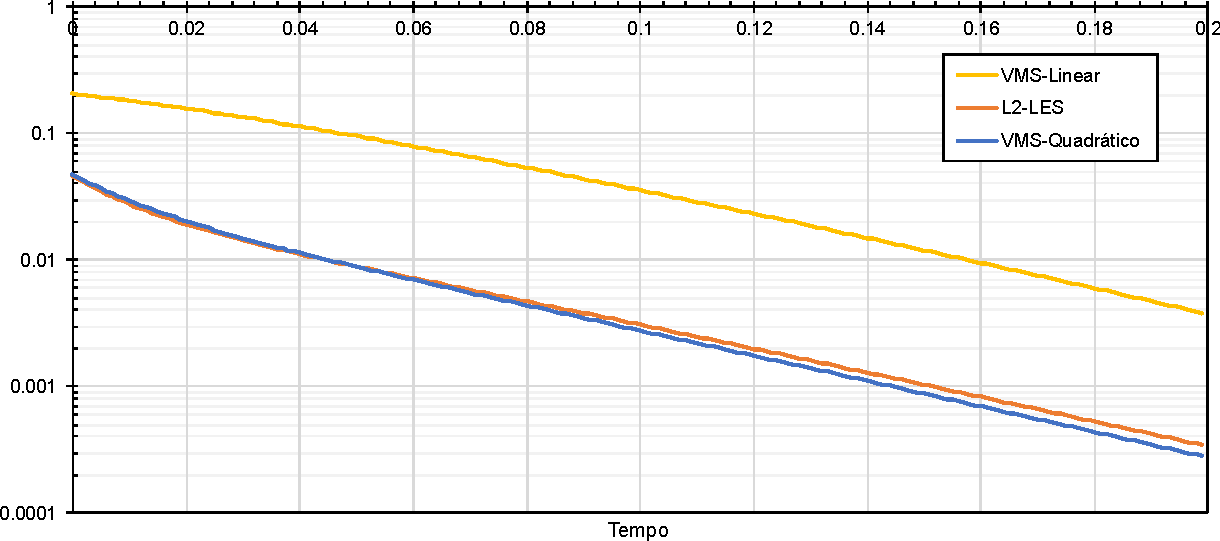
\includegraphics[width=\linewidth]{Figuras/taylor-green/L2.pdf}
    \\Fonte: Autoria Própria (\the\year).
    \label{fig:TGV-L2}
\end{figure}

Assim, observa-se que para o problema estudado, tanto as simulações VMS de aproximação quadrática quanto LES com elemento P2P1 apresentaram boa concordância com o resultado analítico, sendo que ambos apresentaram erros muito próximos entre si, enquanto o VMS de aproximação linear já apresentou um erro maior. Analisando o instante de tempo $t=0.1$ obteve-se um erro $L^2$ de $3,55\times 10^{-2}$, $2,77\times 10^{-3}$ e $3,07\times 10^{-3}$ para as simulações VMS linear, quadrático e LES, respectivamente. Ao verificar a ordem da medida do erro, observa-se que estes valores encontram-se próximos ao obtido por \citeonline{zapata2023parallel}. Realizando uma regressão exponencial do tipo \[\norm{\BB{e}}=a\cdot10^{mt}\] para $t\geq 0,1$, encontra-se $m=-9,80$, $m=-10,01$ e $m=-9,60$ para os respectivos modelos.

%==================================================================================================
\subsubsection{Escoamento sobre um cilindro}
%==================================================================================================

Para o seguinte problema considerou-se um cilindro circular de raio $R=0,5$ em um domínio retangular $\Omega=[0,112R]\times[0,100R]$, sendo o centro do cilindro posicionado sobre o ponto $(36,50)R$. As condições de contorno consideradas foram de entrada na face esquerda ($x_1=0$) do domínio ($\BB{u}=\{u_\infty,0\}^T$), condição de velocidade vertical nula nas faces inferior e superior ($u_2=0$ em $x_2=0$ e $x_2=100R$) e pressão nula no ponto $(112,100)R$. Como condição inicial aplicou-se uma velocidade $\BB{u}=\{u_\infty,0\}^T$ em todo o domínio. A densidade do fluido foi de $\rho=1$ com viscosidade $\nu=0,01$ e uma velocidade $u_\infty=1$, que, ao considerar o comprimento característico como o diâmetro do cilindro, obtém-se $\Rey=100$.

Para a simulação numérica considerou-se a malha apresentada na Figura \ref{fig:cyl-mesh}, a qual possui 4656 elementos finitos. Assim, estudou-se o escoamento em situação onde não se aplicou nenhum modelo de turbulência, seguido da aplicação dos modelos LES e VMS. Todas as simulações foram conduzidas utilizando os elementos de aproximação linear, quadrática e Taylor-Hood P2P1. Para os elementos linear e quadrático aplicou-se em todos os casos o estabilizador PSPG para obtenção de resultados consistentes. O problema discretizado possui 7263 graus de liberdade para elemento linear, 28494 para elemento quadrático e 21417 para P2P1. O intervalo de tempo foi de $t\in[0,200]$ com passos de $\Delta t=0,1$.

\begin{figure}[h!]
    \centering
    \caption{Malha utilizada para a simulação de escoamento sobre um cilindro.}
    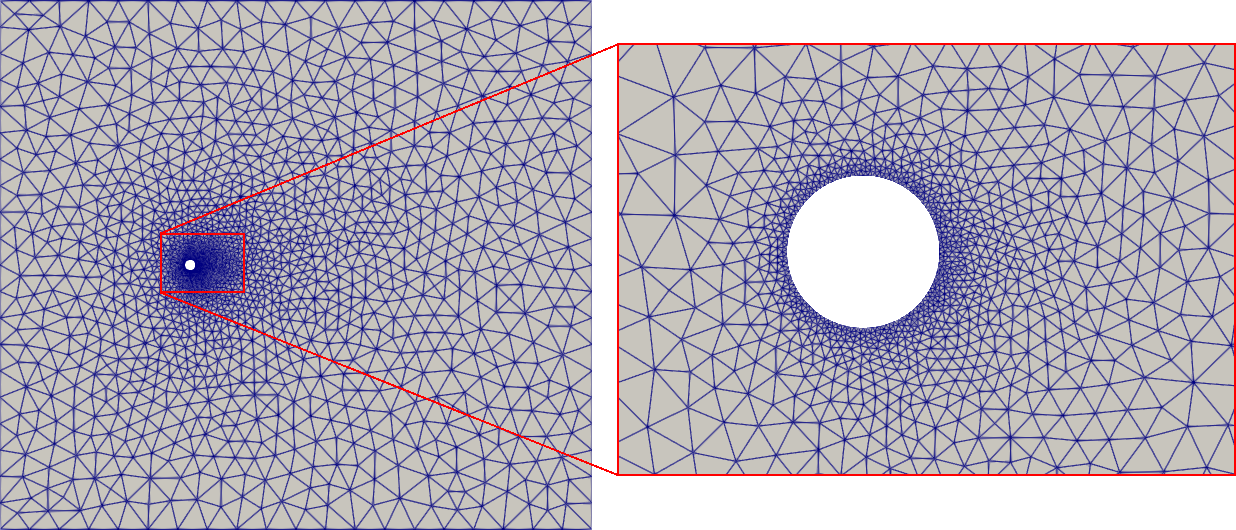
\includegraphics[width=\linewidth]{Figuras/cylinder/analise2/mesh.png}
    \\Fonte: Autoria Própria (\the\year).
    \label{fig:cyl-mesh}
\end{figure}

Para análise dos resultados determinou-se os coeficientes de arrasto (\textit{Drag} - $C_D$) e de sustentação (\textit{Lift} - $C_L$), dados respectivamente por:

\begin{subequations}
    \begin{equation}
        C_D=\frac{2F_D}{\rho\norm{\BB{u}_\infty}^2L}\text{ e}
    \end{equation}
    \begin{equation}
        C_L=\frac{2F_L}{\rho\norm{\BB{u}_\infty}^2L}\text{,}
    \end{equation}
\end{subequations}

\noindent em que $F_D$ e $F_L$ são as forças de arrasto e de sustentação, calculados como:

\begin{subequations}
    \begin{equation}
        F_D=\int_{\Gamma_S}{\sigma_{1j}n_jd\Gamma_S}\text{ e}
    \end{equation}
    \begin{equation}
        F_L=\int_{\Gamma_S}{\sigma_{2j}n_jd\Gamma_S}\text{,}
    \end{equation}
\end{subequations}

\noindent sendo $\Gamma_S$ a fronteira do cilindro e $\BB{n}$ o vetor normal à $\Gamma_S$.

Outro parâmetro possível de se verificar é o número de Strouhal ($\Str$), que se trata de um número adimensional que busca relacionar a frequência de oscilação devido à formação de vórtices e a velocidade do fluido. Esse parâmetro pode ser determinado por:

\begin{equation}
    \Str=\frac{f_vL}{\norm{\BB{u}_\infty}}\text{,}
\end{equation}

\noindent sendo $f_v$ a frequência de desprendimento de vórtices.

As Figuras \ref{fig:cyl-draglift-None}, \ref{fig:cyl-draglift-LES} e \ref{fig:cyl-draglift-VMS} apresentam os coeficientes de arrasto e de sustentação obtidos em todas as simulações. Os campos de velocidades e de pressões atuantes no cilindro no instante $t=120$ são apresentados no Apêndice B.

\begin{figure}[h!]
    \centering
    \caption{Valores ao longo do tempo na simulação sem modelo de:}
    \begin{subfigure}{.49\textwidth}
        \centering
        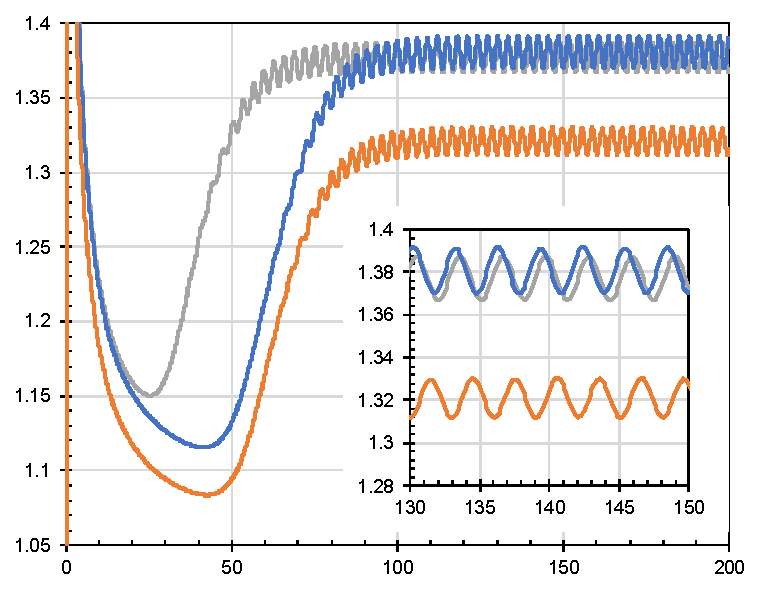
\includegraphics[width=\linewidth]{Figuras/cylinder/analise2/none-drag.pdf}
        \caption{coeficiente de arrasto.}
    \end{subfigure}
    \begin{subfigure}{.49\textwidth}
        \centering
        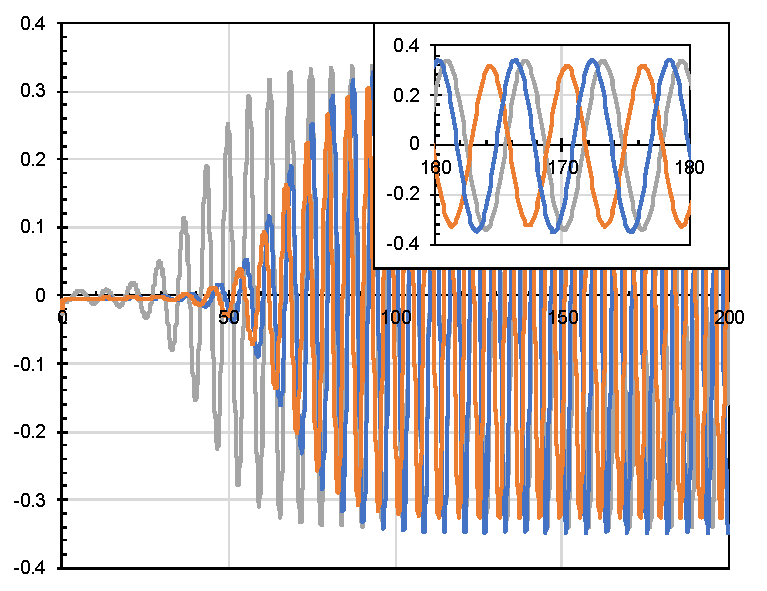
\includegraphics[width=\linewidth]{Figuras/cylinder/analise2/none-lift.pdf}
        \caption{coeficiente de sustentação.}
    \end{subfigure}
    \begin{subfigure}{\textwidth}
        \centering
        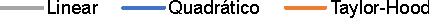
\includegraphics[width=.4\linewidth]{Figuras/cylinder/analise2/legenda.pdf}
    \end{subfigure}
    \\Fonte: Autoria Própria (\the\year).
    \label{fig:cyl-draglift-None}
\end{figure}

\begin{figure}[h!]
    \centering
    \caption{Valores ao longo do tempo na simulação LES de:}
    \begin{subfigure}{.49\textwidth}
        \centering
        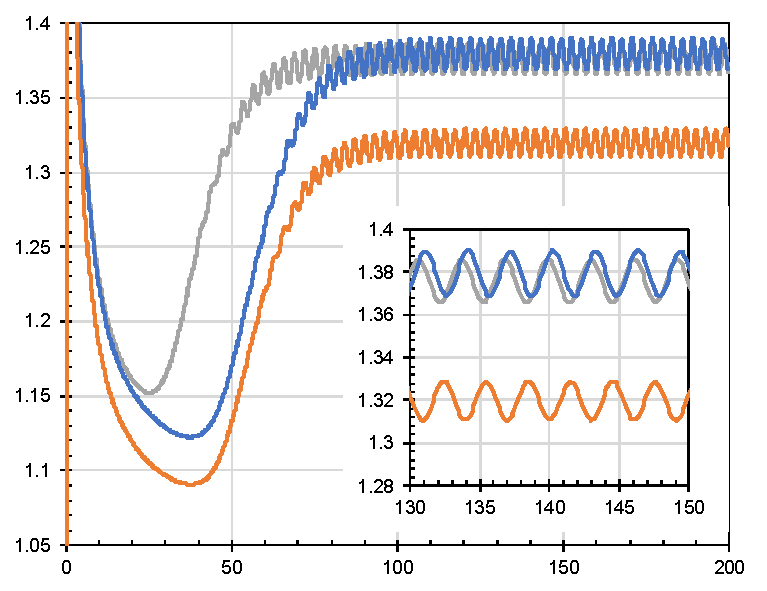
\includegraphics[width=\linewidth]{Figuras/cylinder/analise2/LES-drag.pdf}
        \caption{coeficiente de arrasto.}
    \end{subfigure}
    \begin{subfigure}{.49\textwidth}
        \centering
        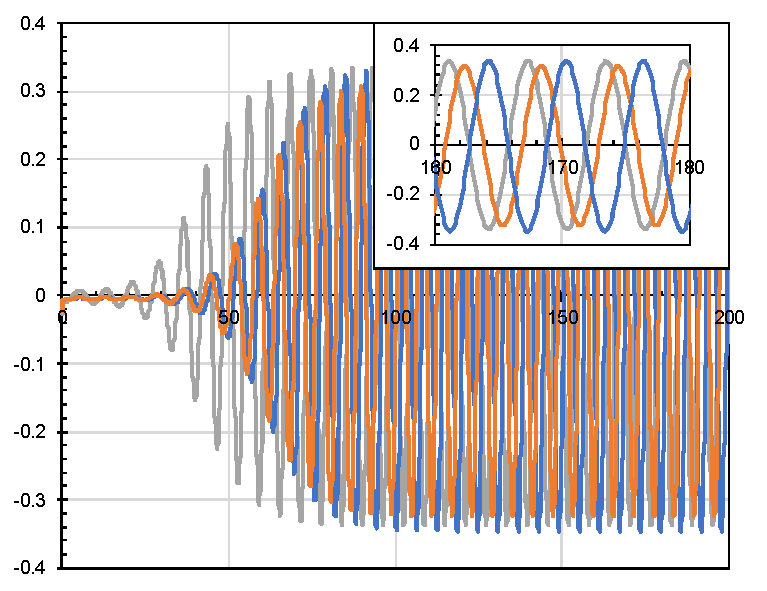
\includegraphics[width=\linewidth]{Figuras/cylinder/analise2/LES-lift.pdf}
        \caption{coeficiente de sustentação.}
    \end{subfigure}
    \begin{subfigure}{\textwidth}
        \centering
        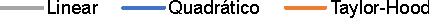
\includegraphics[width=.4\linewidth]{Figuras/cylinder/analise2/legenda.pdf}
    \end{subfigure}
    \\Fonte: Autoria Própria (\the\year).
    \label{fig:cyl-draglift-LES}
\end{figure}

\begin{figure}[h!]
    \centering
    \caption{Valores ao longo do tempo na simulação VMS de:}
    \begin{subfigure}{.49\textwidth}
        \centering
        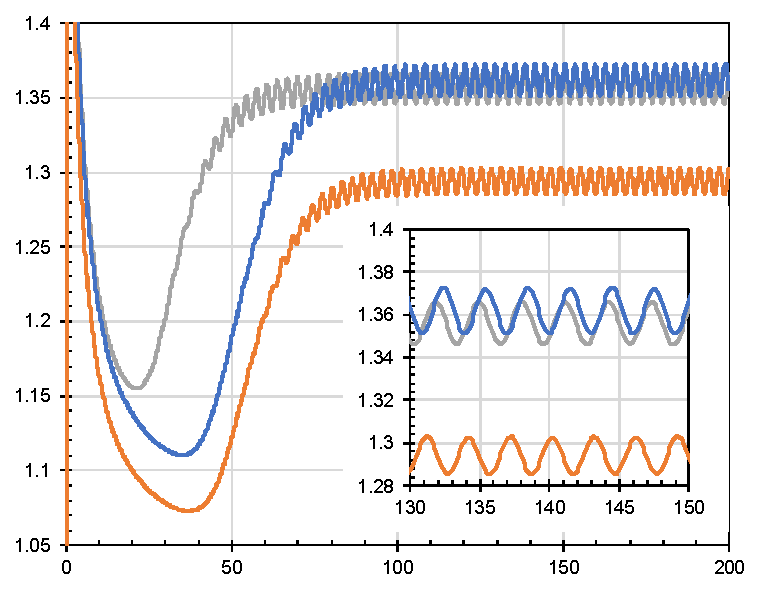
\includegraphics[width=\linewidth]{Figuras/cylinder/analise2/VMS-drag.pdf}
        \caption{coeficiente de arrasto.}
    \end{subfigure}
    \begin{subfigure}{.49\textwidth}
        \centering
        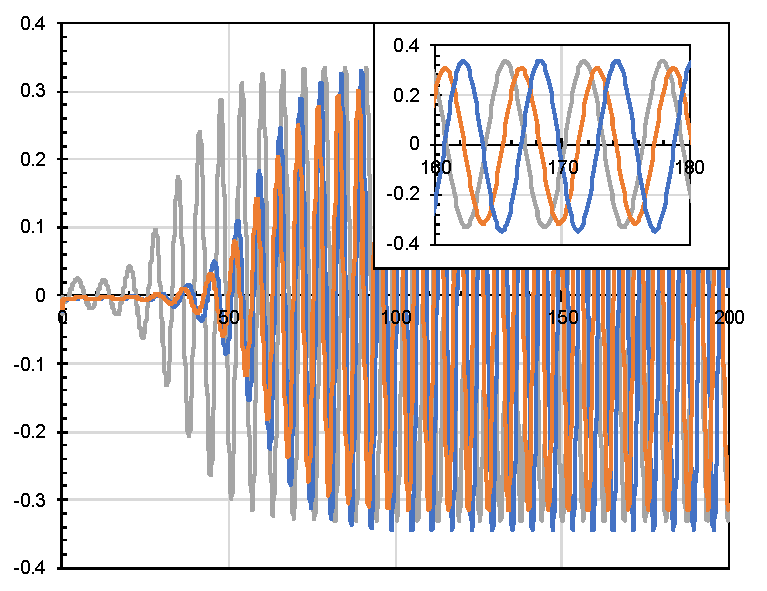
\includegraphics[width=\linewidth]{Figuras/cylinder/analise2/VMS-lift.pdf}
        \caption{coeficiente de sustentação.}
    \end{subfigure}
    \begin{subfigure}{\textwidth}
        \centering
        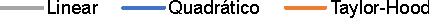
\includegraphics[width=.4\linewidth]{Figuras/cylinder/analise2/legenda.pdf}
    \end{subfigure}
    \\Fonte: Autoria Própria (\the\year).
    \label{fig:cyl-draglift-VMS}
\end{figure}

Os valores da média e da amplitude dos coeficientes de arrasto e de sustentação após o escoamento atingir o equilíbrio dinâmico, assim como o número de Strouhal, são apresentados na Tabela \ref{tab:cyl-res}.

\begin{table}[h!]
    \centering
    \newcommand{\celc}{\multicolumn{1}{c}}
    \newcommand{\ccelc}{\multicolumn{2}{c}}
    \caption{Valores das propriedades dos coeficientes de arrasto e de sustentação para os modelos analisados.}
    \begin{tabular}{llllllll}
        \hline
        \MR{2}{*}{Param.}    & \celc{\MR{2}{*}{Modelo}} & \ccelc{Linear} & \ccelc{Quadrático} & \ccelc{Taylor-Hood}                                           \\\cline{3-8}
                             & \celc{}                  & \celc{Drag}    & \celc{Lift}        & \celc{Drag}         & \celc{Lift} & \celc{Drag} & \celc{Lift} \\\hline
        \MR{3}{*}{Amplitude} & Nenhum                   & 0,0102         & 0,3383             & 0,0109              & 0,3436      & 0,0094      & 0,3219      \\
                             & VMS                      & 0,0101         & 0,3333             & 0,0108              & 0,3411      & 0,0088      & 0,3114      \\
                             & LES                      & 0,0101         & 0,3365             & 0,0107              & 0,3417      & 0,0092      & 0,3200      \\\hline
        \MR{3}{*}{Média}     & Nenhum                   & 1,3772         & -0,0006            & 1,3808              & -0,0080     & 1,3209      & -0,0032     \\
                             & VMS                      & 1,3561         & 0,0046             & 1,3620              & -0,0007     & 1,2939      & -0,0083     \\
                             & LES                      & 1,3760         & -0,0003            & 1,3794              & -0,0031     & 1,3199      & -0,0007     \\\hline
        \MR{3}{*}{Strouhal}  & Nenhum                   & \ccelc{0,1594} & \ccelc{0,1623}     & \ccelc{0,1627}                                                \\
                             & VMS                      & \ccelc{0,1588} & \ccelc{0,1634}     & \ccelc{0,1649}                                                \\
                             & LES                      & \ccelc{0,1590} & \ccelc{0,1614}     & \ccelc{0,1629}                                                \\\hline
    \end{tabular}
    \\Fonte: Autoria Própria (\the\year).
    \label{tab:cyl-res}
\end{table}

Comparando-se os números de Strouhal calculados com aqueles obtidos por \citeonline{fernandes2020tecnica}, que obteve, para a mesma geometria de domínio e mesmas condições de contorno, um $\Str=0,165$ e amplitude do coeficiente de sustentação de 0,3422, \citeonline{tezduyar1992incompressible}, os quais verificaram $\Str$ entre 0,166 e 0,170, \citeonline{najafi2012meshless}, com valor de 0,182, e \citeonline{codina2006numerical}, com velores entre 0,177 e 0,184. As variações observadas entre os números de Strouhal dos diferentes autores podem ser devidas às diferenças nas dimensões dos domínios utilizados, assim como as diferentes condições de contorno aplicadas por cada um. No entanto ainda observa-se que em todos os casos os valores calculados nas simulações ainda são bem próximos. Já com relação à amplitude do coeficiente de sustentação, observa-se que as simulações utilizando elementos quadráticos obtiveram melhor concordância com a obtida por \citeonline{fernandes2020tecnica}. A mínima diferença observada entre os parâmetros calculados em uma simulação sem aplicação de modelo e aquelas que aplicam os modelos VMS e LES, deve-se ao fato do número de Reynolds ser muito baixo, pois, como apontado por \citeonline{fernandes2020tecnica}, esse tipo de escoamento (com $\Rey$ entre 50 e 200) apresenta a formação de vórtices laminares, denominada de esteira de Von Kárman. Para uma verificação mais precisa dessa influência, deve-se partir para uma análise tridimensional com número de Reynolds superiores à 200. Em termos de comparação entre os diferentes tipos de aproximação, verifica-se que tanto os elementos lineares e quadráticos atingiram um regime permanente próximos, enquanto o elemento P2P1 apresentou um amortecimento excessivo, tanto no coeficiente de arrasto, quanto no de sustentação. Já realizando uma comparação dos modelos entre si, verifica-se que em todos os casos o coeficiente de sustentação se manteve inalterado, enquanto o coeficiente de arrasto resultou em uma média menor em relação à simulação LES e sem modelo, porém, mantendo os demais parâmetros muito próximos.

%Vale observar ainda que a simulação VMS linear apresentou um amortecimento menor em relação ao início das oscilações, porém converge para valores muito próximos ao quadrático ao longo do tempo. Já a simulação LES inicia sua oscilação próxima ao VMS quadrático, entretanto com uma média de oscilação menor que a do VMS, em especial ao se observar o coeficiente de arrasto. Tal efeito pode ser devido ao relatado por \citeonline{germano1991dynamic,hughes2000large}, que apontam a ocorrência de um amortecimento excessivo provocado pelo tensor SGS de Smagorinsky.
%==================================================================================================
\subsection{Exemplos Numéricos} \label{ExemplosMT}
%==================================================================================================

Na presente seção serão apresentadas algumas simulações realizadas utilizando os modelos VMS e LES, com a finalidade de validar os modelos implementados.

%==================================================================================================
\subsubsection{Cavidade bidimensional}
%==================================================================================================

A primeira simulação é um problema comumente utilizado na literatura como \textit{benchmark}, o qual trata-se de uma cavidade quadrada ($\Omega=[-1,1]^2$) com paredes aderentes, onde o fluido encontra-se confinado e sujeito a uma velocidade prescrita $\BB{u}_\infty$ ocasionada devido ao deslizamento de uma parede na face superior da cavidade. Nesse sentido serão observados os efeitos provocados no fluido devido à diferentes números de Reynolds, o qual é calculado por meio da equação \ref{eq:Reynolds}:

\begin{equation}
    \Rey=\frac{\rho L\norm{\BB{u}_\infty}}{\mu}\text{,}
    \label{eq:Reynolds}
\end{equation}

\noindent em que $L$ é o comprimento característico, que no caso analisado é igual ao lado da cavidade. Dessa forma considera-se uma velocidade constante para todas as análises de $\BB{u}_\infty=\{1,0\}^T$, sendo os diferentes números de Reynolds obtidos pela variação da viscosidade do fluido. A Figura \ref{fig:cavity} apresenta esquematicamente o problema simulado.

\begin{figure}[h!]
    \centering
    \caption{Desenho esquemático do problema de cavidade.}
    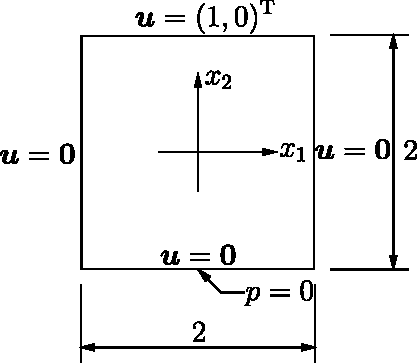
\includegraphics[width=.35\linewidth]{Figuras/Cavity/cavidade.pdf}
    \\Fonte: Autoria Própria (\the\year).
    \label{fig:cavity}
\end{figure}

Pelo fato do problema possuir apenas fronteiras do tipo Dirichlet, o condicionamento da solução do campo de pressões é garantido pela aplicação de uma condição de pressão nula no vértice superior direito da cavidade, conforme visto na figura acima.  Também se observa que existe uma descontinuidade nas condições de contorno no encontro entre as paredes da cavidade e seu topo, podendo ser consideradas velocidades nulas ou igual à velocidade do topo. No problema em questão considerou-se que a velocidade nesse ponto é igual à $\BB{u}_\infty$.

A malha de elementos finitos foi feita pela subdivisão do domínio em 20000 elementos dispostos de maneira estruturada com orientação à esquerda, conforme observado na Figura \ref{fig:cavity_disc}. O número de graus de liberdade para a simulação VMS de aproximação linear, quadrática e LES são 30603, 121203 e 91003, respectivamente. Os parâmetros utilizados foram $\rho=1$ para todas as análises, $\mu=0,02$, $\mu=5\times10^{-3}$, $\mu=2\times10^{-3}$, $\mu=4\times10^{-4}$, $\mu=2,6667\times10^{-4}$ e $\mu=2\times10^{-4}$, resultando em $\Rey=100$, $\Rey=400$, $\Rey=1000$, $\Rey=5000$, $\Rey=7500$ e $\Rey=10000$, respectivamente. Os modelos utilizados foram o VMS com aproximação linear e quadrática e o LES com elementos de Taylor-Hood P2P1 e $C_S=0,10$. O passo de tempo em todos os casos foi de $\Delta t=0,1$ e a simulação foi mantida até que a estacionariedade dos parâmetros do fluxo fosse alcançada.

\begin{figure}[h!]
    \centering
    \caption{Malha considerada para o problema de cavidade.}
    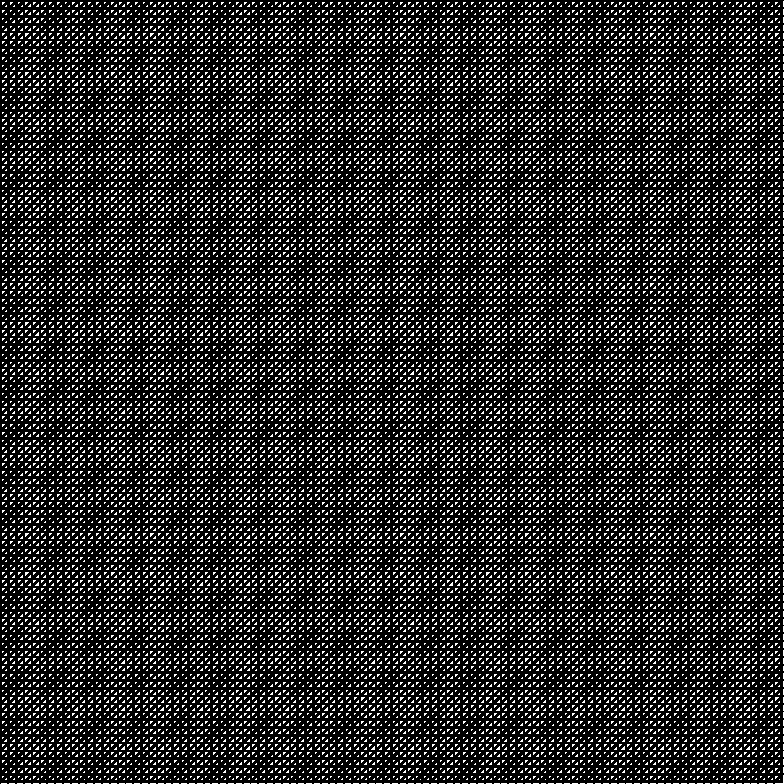
\includegraphics[width=.6\linewidth]{Figuras/Cavity/mesh.pdf}
    \\Fonte: Autoria Própria (\the\year).
    \label{fig:cavity_disc}
\end{figure}

Como o problema apresenta características de um escoamento quase-estático, a parcela dos termos inerciais foram desprezados em ambos os modelos de turbulência. Além disso, os resultados adquiridos para um determinado número de Reynolds foram aplicados como valores iniciais para a determinação dos resultados para a próxima análise.

Os resultados obtidos foram comparados com aqueles apresentados por \citeonline{ghia1982high}. A Figura \ref{fig:cavity-results} apresenta os valores do campo de velocidades sobre as linhas médias da cavidade ($x_1=0$ e $x_2=0$).

\begin{figure}[h!]
    \centering
    \caption{Valores do campo de velocidades sobre as linhas médias da cavidade.}
    \begin{subfigure}{0.4\textwidth}
        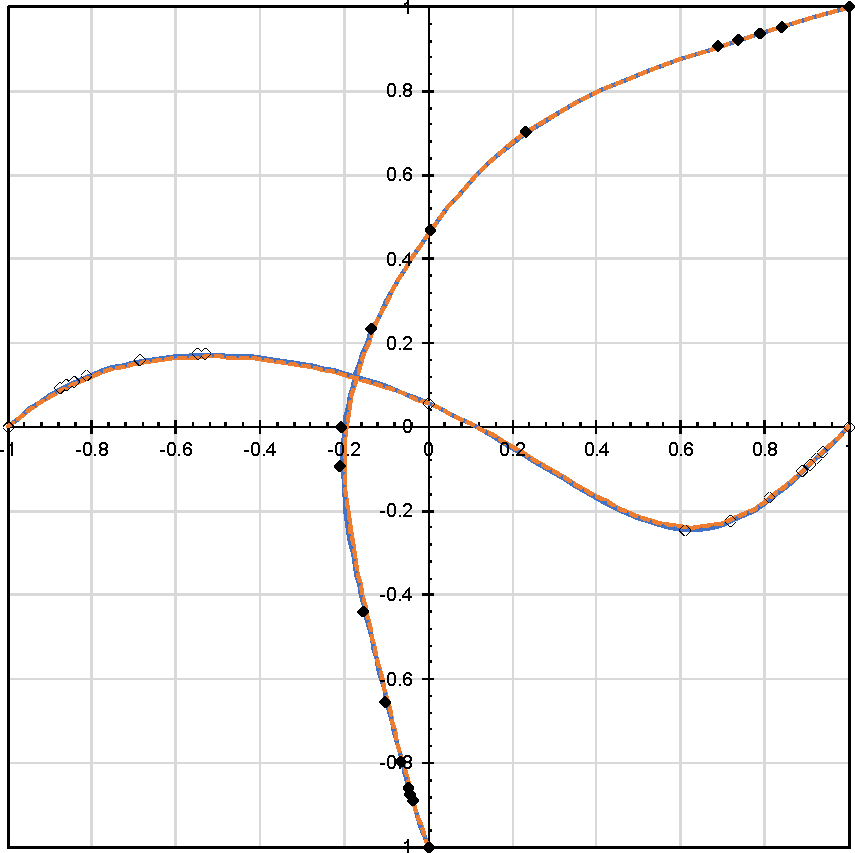
\includegraphics[width=\linewidth]{Figuras/Cavity/Re100.pdf}
        \caption{$\Rey=100$}
    \end{subfigure}
    \begin{subfigure}{0.4\textwidth}
        \includegraphics[width=\linewidth]{Figuras/Cavity/Re400.pdf}
        \caption{$\Rey=400$}
    \end{subfigure}
    \begin{subfigure}{0.4\textwidth}
        \includegraphics[width=\linewidth]{Figuras/Cavity/Re1000.pdf}
        \caption{$\Rey=1000$}
    \end{subfigure}
    \begin{subfigure}{0.4\textwidth}
        \includegraphics[width=\linewidth]{Figuras/Cavity/Re5000.pdf}
        \caption{$\Rey=5000$}
    \end{subfigure}
    \begin{subfigure}{0.4\textwidth}
        \includegraphics[width=\linewidth]{Figuras/Cavity/Re7500.pdf}
        \caption{$\Rey=7500$}
    \end{subfigure}
    \begin{subfigure}{0.4\textwidth}
        \includegraphics[width=\linewidth]{Figuras/Cavity/Re10000.pdf}
        \caption{$\Rey=10000$}
    \end{subfigure}
    \begin{subfigure}{\textwidth}
        \includegraphics[width=\linewidth]{Figuras/Cavity/Legenda.pdf}
    \end{subfigure}
    \\Fonte: Autoria Própria (\the\year).
    \label{fig:cavity-results}
\end{figure}

A Figura \ref{fig:cavity-results2} apresenta o campo de velocidades na cavidade após o escoamento atingir seu estado estacionário.

\begin{figure}[h!]
    \centering
    \caption{Campo de velocidades em regime estacionário na cavidade.}
    \begin{subfigure}{0.32\textwidth}
        \includegraphics[width=\linewidth]{Figuras/Cavity/Re100.png}
        \caption{$\Rey=100$}
    \end{subfigure}
    \begin{subfigure}{0.32\textwidth}
        \includegraphics[width=\linewidth]{Figuras/Cavity/Re400.png}
        \caption{$\Rey=400$}
    \end{subfigure}
    \begin{subfigure}{0.32\textwidth}
        \includegraphics[width=\linewidth]{Figuras/Cavity/Re1000.png}
        \caption{$\Rey=1000$}
    \end{subfigure}
    \begin{subfigure}{0.32\textwidth}
        \includegraphics[width=\linewidth]{Figuras/Cavity/Re5000.png}
        \caption{$\Rey=5000$}
    \end{subfigure}
    \begin{subfigure}{0.32\textwidth}
        \includegraphics[width=\linewidth]{Figuras/Cavity/Re7500.png}
        \caption{$\Rey=7500$}
    \end{subfigure}
    \begin{subfigure}{0.32\textwidth}
        \includegraphics[width=\linewidth]{Figuras/Cavity/Re10000.png}
        \caption{$\Rey=10000$}
    \end{subfigure}
    \begin{subfigure}{0.4\textwidth}
        \includegraphics[width=\linewidth]{Figuras/Cavity/Legenda.png}
    \end{subfigure}
    \\Fonte: Autoria Própria (\the\year).
    \label{fig:cavity-results2}
\end{figure}

Para todas as simulações conduzidas, percebeu-se que houve uma excelente concordância dos resultados para números de Reynolds baixos, no entanto a simulação VMS de aproximação linear passou a apresentar resultados cada vez mais discrepantes à medida que o número de Reynolds aumentou, enquanto o VMS de aproximação quadrática e o LES apresentaram resultados mais próximos aos de \citeonline{ghia1982high}, sendo que o LES apresentou resultados ligeiramente melhores em relação ao VMS quadrático. Para número de Reynolds muito altos observou-se um leve desvio nos resultados próximos à parede superior da cavidade, o que poderia ser melhorado caso uma discretização mais fina da malha fosse empregada nessa região.

Para comparação da convergência entre os modelos implementados realizou-se um simulação com $\Rey=1000$ partindo de uma condição inicial $\BB{u}=\BB{0}$ em todo o domínio. As medidas de resíduos observadas foram relacionadas à velocidade ($e_u=\norm{\Delta\BB{U}}$) e à pressão ($e_p=\norm{\Delta\BB{P}}$) e a simulação foi conduzida até que um resíduo abaixo de $1\times10^{-8}$ fosse obtido. A Figura \ref{fig:comp-res} apresenta a convergência dos modelos segundo essas medidas.

\begin{figure}[h!]
    \centering
    \caption{Comparação do resíduo da:}
    \begin{subfigure}{\textwidth}
        \includegraphics[width=\linewidth]{Figuras/Cavity/resvel.pdf}
        \caption{velocidade.}
    \end{subfigure}
    \begin{subfigure}{\textwidth}
        \includegraphics[width=\linewidth]{Figuras/Cavity/respre.pdf}
        \caption{pressão.}
    \end{subfigure}
    \\Fonte: Autoria Própria (\the\year).
    \label{fig:comp-res}
\end{figure}

Também foi observado o tempo necessário para que a convergência fosse atingida. A Tabela \ref{tab:comp-res} apresenta o número de iteração necessárias para que ambas as medidas de erro atingissem a tolerância, o tempo médio por iteração e o tempo total da simulação.

\begin{table}[h!]
    \centering
    \caption{Resultados do estudo de convergência dos métodos.}
    \begin{tabular}{lccc}
        \hline
        Modelo         & número de iterações & tempo por iteração (s) & tempo (min) \\\hline
        VMS linear     & 3218                & 0,650                  & 34,872      \\
        VMS quadrático & 2788                & 3,814                  & 177,260     \\
        LES            & 3182                & 3,494                  & 185,357     \\\hline
    \end{tabular}
    \\Fonte: Autoria Própria (\the\year).
    \label{tab:comp-res}
\end{table}

Observa-se no resíduo da velocidade que todos os métodos tiveram uma convergência mais rápida no início da simulação, pois um fluxo rotacional ainda estava sendo obtido pelos modelos. Após se estabelecer esse fluxo a convergência desacelerou até atingir a tolerância admitida. Já com relação ao resíduo da pressão verifica-se que o modelo LES obteve uma convergência imediata, no entanto a convergência dos demais modelos também foi rápida de tal forma a essa medida não ser o limitante em relação ao tempo de processamento. Ao final do processamento o VMS quadrático foi o que precisou da menor quantidade de iterações para convergir, no entanto, devido à quantidade de graus de liberdade ser maior, seu tempo requerido para cada iteração aumentou, necessitando de um tempo similar ao LES.

Por fim, verificou-se a necessidade da utilização do modelo de turbulência em simulações de malha menos refinada em situação de número de Reynolds elevado. Para isso assumiu-se um problema com $\Rey=10000$, sendo o domínio computacional gerado pela divisão de cada aresta em 20 segmentos, totalizando, assim, 800 elementos finitos triangulares, dispostos de forma estruturada com orientação à esquerda. As simulações foram conduzidas sem a utilização de nenhum modelo de turbulência, seguido dos modelos LES e VMS. Para cada uma das simulações empregou-se elementos de aproximação linear, quadrática e Taylor-Hood P2P1, sendo que para os dois primeiros aplicou-se um estabilizador PSPG, uma vez que esses elementos não possuem estabilidade no campo de pressões. Assim, chegou-se em 441 nós e 1323 DOF para a simulação contendo elementos lineares, 1681 nós e 5043 DOF para quadráticos e 1681 nós e 3803 DOF para P2P1. A simulação foi mantida em um intervalo de tempo $t\in[0,500]$, discretizado em $\Delta t=0,1$, sendo que a condição inicial foi de $\BB{u}=\BB{0}$ em todos os pontos no interior do domínio. A Tabela \ref{tab:comp-res2} apresenta de forma qualitativa os resultados obtidos. O campo de velocidades obtidos para cada simulação no instante $t=500$ é apresentado no Apêndice A.

\begin{table}[h!]
    \centering
    \caption{Comparação dos resultados apresentados em simulação em modelo, com aplicação de LES e de VMS.}
    \begin{tabularx}{\textwidth}{|p{2cm}|p{3cm}|X|}
        \hline
        Tipo de elemento      & Simulação  & Resultado                                                         \\\hline
        \MR{3}{*}{Linear}     & Sem modelo & Sem sentido físico                                                \\\cline{2-3}
                              & LES        & Formação de vórtice com valores espúrios próximos à face superior \\\cline{2-3}
                              & VMS        & Formação de vórtice com variação pequena do campo de velocidades  \\\hline
        \MR{3}{*}{Quadrático} & Sem modelo & Não houve avanço na solução (se manteve na condição inicial)      \\\cline{2-3}
                              & LES        & Formação de vórtice                                               \\\cline{2-3}
                              & VMS        & Formação de vórtice                                               \\\hline
        \MR{3}{*}{P2P1}       & Sem modelo & Divergência                                                       \\\cline{2-3}
                              & LES        & Não atingiu o regime permanente                                   \\\cline{2-3}
                              & VMS        & Formação de vórtice                                               \\\hline
    \end{tabularx}
    \\Fonte: Autoria Própria (\the\year).
    \label{tab:comp-res2}
\end{table}

Logo, verifica-se que as simulações sem a aplicação de modelos de turbulência não foi capaz de simular o comportamento do escoamento. Por outro lado, mesmo em uma situação de malha grosseira, as simulações empregando LES e VMS foram capazes de capturar esse comportamento. No entanto a simulação modelada por LES em elemento P2P1 não atingiu o regime permanente.

%==================================================================================================
\subsubsection{\textit{Taylor-Green Vortex} tridimensional}
%==================================================================================================

Para verificação dos modelos implementados em simulações tridimensionais é possível simular o problema de \textit{Taylor-Green Vortex} (TGV), o qual possui solução analítica, dada por \cite{shapiro1993use}:

\begin{subequations}
    \begin{equation}
        \begin{split}
            &\BB{u}_a(\BB{x},t)=\\
            &-\frac{Ae^{-\nu\lambda^2t}}{k^2+l^2}\begin{bmatrix}
                \lambda l\cos{(kx_1)}\sin{(lx_2)}\sin{(mx_3)}+mk\sin{(kx_1)}\cos{(lx_2)}\cos{(mx_3)} \\
                \lambda k\sin{(kx_1)}\cos{(lx_2)}\sin{(mx_3)}-ml\cos{(kx_1)}\sin{(lx_2)}\cos{(mx_3)} \\
                -(k^2+l^2)\cos{(kx_1)}\cos{(lx_2)}\sin{(mx_3)}
            \end{bmatrix}\text{,}
        \end{split}
    \end{equation}
    \begin{equation}
        p_a=p_s-\rho\frac{u_1^2+u_2+u_3^2}{2}\text{.}
    \end{equation}
\end{subequations}

\noindent em que $k$, $l$ e $m$ são constantes arbitrárias, $\lambda^2=k^2+l^2+m^2$, $A$ é a amplitude da componente $u_3$ e $p_s$ é a pressão do ponto de estagnação.

Para o problema numérico foi considerado um cubo ($\Omega=[-1,1]^3$) simulado nos modelos VMS de aproximação linear e quadrática e o LES utilizando elementos Taylor-Hood P2P1. A malha utilizada na discretização conta com 5802 elementos finitos (conforme ilustrado na Figura \ref{fig:TGV-mesh}), sendo 5580 graus de liberdade para VMS linear, 37600 pra VMS quadrático e 29595 para LES.

\begin{figure}[h!]
    \centering
    \caption{Malha utilizada para a simulação de TGV.}
    \includegraphics[width=0.4\linewidth]{Figuras/taylor-green/mesh.png}
    \\Fonte: Autoria Própria (\the\year).
    \label{fig:TGV-mesh}
\end{figure}

Como condição inicial impôs-se acelerações, velocidade e pressões iguais à solução analítica com $t=0$ e como condições de contorno aplicou-se velocidades iguais à analítica em toda a fronteira e $p=0$ no centro do domínio. Os valores dos parâmetros foram $k=l=m=\pi$ e $A=\nu=\rho=1$, sendo o período analisado de $t\in[0,0.2]$ com um passo de tempo de $\Delta t=0.001$.

Sendo assim, a Figura \ref{fig:TGV-results} apresenta os valores do campo de velocidades nas linhas $x_2=x_3=0$ ($l1$), $x_1=x_3=0$ ($l2$) e $x_1=x_2=0$ ($l3$) para os instantes $t=0$, $t=0.05$ e $t=0.2$ para todos os modelos considerados.

\begin{figure}[h!]
    \centering
    \caption{Velocidades obtidas na a simulação de TGV em:}
    \begin{subfigure}{0.42\textwidth}
        \includegraphics[width=\linewidth]{Figuras/taylor-green/VMS-Lin.pdf}
        \caption{$l1$ e $l2$ para VMS linear.}
    \end{subfigure}
    \begin{subfigure}{0.42\textwidth}
        \includegraphics[width=\linewidth]{Figuras/taylor-green/VMS-Lin-uz.pdf}
        \caption{$l3$ para VMS linear.}
    \end{subfigure}
    \begin{subfigure}{0.42\textwidth}
        \includegraphics[width=\linewidth]{Figuras/taylor-green/VMS-Qua.pdf}
        \caption{$l1$ e $l2$ para VMS quadrático.}
    \end{subfigure}
    \begin{subfigure}{0.42\textwidth}
        \includegraphics[width=\linewidth]{Figuras/taylor-green/VMS-Qua-uz.pdf}
        \caption{$l3$ para VMS quadrático.}
    \end{subfigure}
    \begin{subfigure}{0.42\textwidth}
        \includegraphics[width=\linewidth]{Figuras/taylor-green/LES.pdf}
        \caption{$l1$ e $l2$ para LES.}
    \end{subfigure}
    \begin{subfigure}{0.42\textwidth}
        \includegraphics[width=\linewidth]{Figuras/taylor-green/LES-uz.pdf}
        \caption{$l3$ para LES.}
    \end{subfigure}
    \begin{subfigure}{0.42\textwidth}
        \includegraphics[width=\linewidth]{Figuras/taylor-green/legenda.pdf}
    \end{subfigure}
    \\Fonte: Autoria Própria (\the\year).
    \label{fig:TGV-results}
\end{figure}

Para comparação com a solução analítica, tomou-se a medida do erro em $L^2$, expresso por \cite{dumon2011proper}:

\begin{equation}
    \norm{\BB{e}}=\norm{\BB{u}-\BB{u}_a}_{L^\infty(L^2(\Omega))}=\max_{0<t\leq T}{\left[\int_\Omega{\norm{\BB{u}-\BB{u}_a}^2d\Omega}\right]}\text{,}
\end{equation}

\noindent o qual é representado ao longo do tempo de acordo com a Figura \ref{fig:TGV-L2}:

\begin{figure}[h!]
    \centering
    \caption{Medidas de $L^2$ ao longo do tempo.}
    \includegraphics[width=\linewidth]{Figuras/taylor-green/L2.pdf}
    \\Fonte: Autoria Própria (\the\year).
    \label{fig:TGV-L2}
\end{figure}

Assim, observa-se que para o problema estudado, tanto as simulações VMS de aproximação quadrática quanto LES com elemento P2P1 apresentaram boa concordância com o resultado analítico, sendo que ambos apresentaram erros muito próximos entre si, enquanto o VMS de aproximação linear já apresentou um erro maior. Analisando o instante de tempo $t=0.1$ obteve-se um erro $L^2$ de $3,55\times 10^{-2}$, $2,77\times 10^{-3}$ e $3,07\times 10^{-3}$ para as simulações VMS linear, quadrático e LES, respectivamente. Ao verificar a ordem da medida do erro, observa-se que estes valores encontram-se próximos ao obtido por \citeonline{zapata2023parallel}. Realizando uma regressão exponencial do tipo \[\norm{\BB{e}}=a\cdot10^{mt}\] para $t\geq 0,1$, encontra-se $m=-9,80$, $m=-10,01$ e $m=-9,60$ para os respectivos modelos.

%==================================================================================================
\subsubsection{Escoamento sobre um cilindro}
%==================================================================================================

Para o seguinte problema considerou-se um cilindro circular de raio $R=0,5$ em um domínio retangular $\Omega=[0,112R]\times[0,100R]$, sendo o centro do cilindro posicionado sobre o ponto $(36,50)R$. As condições de contorno consideradas foram de entrada na face esquerda ($x_1=0$) do domínio ($\BB{u}=\{u_\infty,0\}^T$), condição de velocidade vertical nula nas faces inferior e superior ($u_2=0$ em $x_2=0$ e $x_2=100R$) e pressão nula no ponto $(112,100)R$. Como condição inicial aplicou-se uma velocidade $\BB{u}=\{u_\infty,0\}^T$ em todo o domínio. A densidade do fluido foi de $\rho=1$ com viscosidade $\nu=0,01$ e uma velocidade $u_\infty=1$, que, ao considerar o comprimento característico como o diâmetro do cilindro, obtém-se $\Rey=100$.

Para a simulação numérica considerou-se a malha apresentada na Figura \ref{fig:cyl-mesh}, a qual possui 4656 elementos finitos. Assim, estudou-se o escoamento em situação onde não se aplicou nenhum modelo de turbulência, seguido da aplicação dos modelos LES e VMS. Todas as simulações foram conduzidas utilizando os elementos de aproximação linear, quadrática e Taylor-Hood P2P1. Para os elementos linear e quadrático aplicou-se em todos os casos o estabilizador PSPG para obtenção de resultados consistentes. O problema discretizado possui 7263 graus de liberdade para elemento linear, 28494 para elemento quadrático e 21417 para P2P1. O intervalo de tempo foi de $t\in[0,200]$ com passos de $\Delta t=0,1$.

\begin{figure}[h!]
    \centering
    \caption{Malha utilizada para a simulação de escoamento sobre um cilindro.}
    \includegraphics[width=\linewidth]{Figuras/cylinder/analise2/mesh.png}
    \\Fonte: Autoria Própria (\the\year).
    \label{fig:cyl-mesh}
\end{figure}

Para análise dos resultados determinou-se os coeficientes de arrasto (\textit{Drag} - $C_D$) e de sustentação (\textit{Lift} - $C_L$), dados respectivamente por:

\begin{subequations}
    \begin{equation}
        C_D=\frac{2F_D}{\rho\norm{\BB{u}_\infty}^2L}\text{ e}
    \end{equation}
    \begin{equation}
        C_L=\frac{2F_L}{\rho\norm{\BB{u}_\infty}^2L}\text{,}
    \end{equation}
\end{subequations}

\noindent em que $F_D$ e $F_L$ são as forças de arrasto e de sustentação, calculados como:

\begin{subequations}
    \begin{equation}
        F_D=\int_{\Gamma_S}{\sigma_{1j}n_jd\Gamma_S}\text{ e}
    \end{equation}
    \begin{equation}
        F_L=\int_{\Gamma_S}{\sigma_{2j}n_jd\Gamma_S}\text{,}
    \end{equation}
\end{subequations}

\noindent sendo $\Gamma_S$ a fronteira do cilindro e $\BB{n}$ o vetor normal à $\Gamma_S$.

Outro parâmetro possível de se verificar é o número de Strouhal ($\Str$), que se trata de um número adimensional que busca relacionar a frequência de oscilação devido à formação de vórtices e a velocidade do fluido. Esse parâmetro pode ser determinado por:

\begin{equation}
    \Str=\frac{f_vL}{\norm{\BB{u}_\infty}}\text{,}
\end{equation}

\noindent sendo $f_v$ a frequência de desprendimento de vórtices.

As Figuras \ref{fig:cyl-draglift-None}, \ref{fig:cyl-draglift-LES} e \ref{fig:cyl-draglift-VMS} apresentam os coeficientes de arrasto e de sustentação obtidos em todas as simulações. Os campos de velocidades e de pressões atuantes no cilindro no instante $t=120$ são apresentados no Apêndice B.

\begin{figure}[h!]
    \centering
    \caption{Valores ao longo do tempo na simulação sem modelo de:}
    \begin{subfigure}{.49\textwidth}
        \centering
        \includegraphics[width=\linewidth]{Figuras/cylinder/analise2/none-drag.pdf}
        \caption{coeficiente de arrasto.}
    \end{subfigure}
    \begin{subfigure}{.49\textwidth}
        \centering
        \includegraphics[width=\linewidth]{Figuras/cylinder/analise2/none-lift.pdf}
        \caption{coeficiente de sustentação.}
    \end{subfigure}
    \begin{subfigure}{\textwidth}
        \centering
        \includegraphics[width=.4\linewidth]{Figuras/cylinder/analise2/legenda.pdf}
    \end{subfigure}
    \\Fonte: Autoria Própria (\the\year).
    \label{fig:cyl-draglift-None}
\end{figure}

\begin{figure}[h!]
    \centering
    \caption{Valores ao longo do tempo na simulação LES de:}
    \begin{subfigure}{.49\textwidth}
        \centering
        \includegraphics[width=\linewidth]{Figuras/cylinder/analise2/LES-drag.pdf}
        \caption{coeficiente de arrasto.}
    \end{subfigure}
    \begin{subfigure}{.49\textwidth}
        \centering
        \includegraphics[width=\linewidth]{Figuras/cylinder/analise2/LES-lift.pdf}
        \caption{coeficiente de sustentação.}
    \end{subfigure}
    \begin{subfigure}{\textwidth}
        \centering
        \includegraphics[width=.4\linewidth]{Figuras/cylinder/analise2/legenda.pdf}
    \end{subfigure}
    \\Fonte: Autoria Própria (\the\year).
    \label{fig:cyl-draglift-LES}
\end{figure}

\begin{figure}[h!]
    \centering
    \caption{Valores ao longo do tempo na simulação VMS de:}
    \begin{subfigure}{.49\textwidth}
        \centering
        \includegraphics[width=\linewidth]{Figuras/cylinder/analise2/VMS-drag.pdf}
        \caption{coeficiente de arrasto.}
    \end{subfigure}
    \begin{subfigure}{.49\textwidth}
        \centering
        \includegraphics[width=\linewidth]{Figuras/cylinder/analise2/VMS-lift.pdf}
        \caption{coeficiente de sustentação.}
    \end{subfigure}
    \begin{subfigure}{\textwidth}
        \centering
        \includegraphics[width=.4\linewidth]{Figuras/cylinder/analise2/legenda.pdf}
    \end{subfigure}
    \\Fonte: Autoria Própria (\the\year).
    \label{fig:cyl-draglift-VMS}
\end{figure}

Os valores da média e da amplitude dos coeficientes de arrasto e de sustentação após o escoamento atingir o equilíbrio dinâmico, assim como o número de Strouhal, são apresentados na Tabela \ref{tab:cyl-res}.

\begin{table}[h!]
    \centering
    \newcommand{\celc}{\multicolumn{1}{c}}
    \newcommand{\ccelc}{\multicolumn{2}{c}}
    \caption{Valores das propriedades dos coeficientes de arrasto e de sustentação para os modelos analisados.}
    \begin{tabular}{llllllll}
        \hline
        \MR{2}{*}{Param.}    & \celc{\MR{2}{*}{Modelo}} & \ccelc{Linear} & \ccelc{Quadrático} & \ccelc{Taylor-Hood}                                           \\\cline{3-8}
                             & \celc{}                  & \celc{Drag}    & \celc{Lift}        & \celc{Drag}         & \celc{Lift} & \celc{Drag} & \celc{Lift} \\\hline
        \MR{3}{*}{Amplitude} & Nenhum                   & 0,0102         & 0,3383             & 0,0109              & 0,3436      & 0,0094      & 0,3219      \\
                             & VMS                      & 0,0101         & 0,3333             & 0,0108              & 0,3411      & 0,0088      & 0,3114      \\
                             & LES                      & 0,0101         & 0,3365             & 0,0107              & 0,3417      & 0,0092      & 0,3200      \\\hline
        \MR{3}{*}{Média}     & Nenhum                   & 1,3772         & -0,0006            & 1,3808              & -0,0080     & 1,3209      & -0,0032     \\
                             & VMS                      & 1,3561         & 0,0046             & 1,3620              & -0,0007     & 1,2939      & -0,0083     \\
                             & LES                      & 1,3760         & -0,0003            & 1,3794              & -0,0031     & 1,3199      & -0,0007     \\\hline
        \MR{3}{*}{Strouhal}  & Nenhum                   & \ccelc{0,1594} & \ccelc{0,1623}     & \ccelc{0,1627}                                                \\
                             & VMS                      & \ccelc{0,1588} & \ccelc{0,1634}     & \ccelc{0,1649}                                                \\
                             & LES                      & \ccelc{0,1590} & \ccelc{0,1614}     & \ccelc{0,1629}                                                \\\hline
    \end{tabular}
    \\Fonte: Autoria Própria (\the\year).
    \label{tab:cyl-res}
\end{table}

Comparando-se os números de Strouhal calculados com aqueles obtidos por \citeonline{fernandes2020tecnica}, que obteve, para a mesma geometria de domínio e mesmas condições de contorno, um $\Str=0,165$ e amplitude do coeficiente de sustentação de 0,3422, \citeonline{tezduyar1992incompressible}, os quais verificaram $\Str$ entre 0,166 e 0,170, \citeonline{najafi2012meshless}, com valor de 0,182, e \citeonline{codina2006numerical}, com velores entre 0,177 e 0,184. As variações observadas entre os números de Strouhal dos diferentes autores podem ser devidas às diferenças nas dimensões dos domínios utilizados, assim como as diferentes condições de contorno aplicadas por cada um. No entanto ainda observa-se que em todos os casos os valores calculados nas simulações ainda são bem próximos. Já com relação à amplitude do coeficiente de sustentação, observa-se que as simulações utilizando elementos quadráticos obtiveram melhor concordância com a obtida por \citeonline{fernandes2020tecnica}. A mínima diferença observada entre os parâmetros calculados em uma simulação sem aplicação de modelo e aquelas que aplicam os modelos VMS e LES, deve-se ao fato do número de Reynolds ser muito baixo, pois, como apontado por \citeonline{fernandes2020tecnica}, esse tipo de escoamento (com $\Rey$ entre 50 e 200) apresenta a formação de vórtices laminares, denominada de esteira de Von Kárman. Para uma verificação mais precisa dessa influência, deve-se partir para uma análise tridimensional com número de Reynolds superiores à 200. Em termos de comparação entre os diferentes tipos de aproximação, verifica-se que tanto os elementos lineares e quadráticos atingiram um regime permanente próximos, enquanto o elemento P2P1 apresentou um amortecimento excessivo, tanto no coeficiente de arrasto, quanto no de sustentação. Já realizando uma comparação dos modelos entre si, verifica-se que em todos os casos o coeficiente de sustentação se manteve inalterado, enquanto o coeficiente de arrasto resultou em uma média menor em relação à simulação LES e sem modelo, porém, mantendo os demais parâmetros muito próximos.

%Vale observar ainda que a simulação VMS linear apresentou um amortecimento menor em relação ao início das oscilações, porém converge para valores muito próximos ao quadrático ao longo do tempo. Já a simulação LES inicia sua oscilação próxima ao VMS quadrático, entretanto com uma média de oscilação menor que a do VMS, em especial ao se observar o coeficiente de arrasto. Tal efeito pode ser devido ao relatado por \citeonline{germano1991dynamic,hughes2000large}, que apontam a ocorrência de um amortecimento excessivo provocado pelo tensor SGS de Smagorinsky.